%%%%%%%%%%%%%%%%%%%%%%%%%%%%%%%%%%%%%%%%%%%%%%%
% LATEX UT THESIS TEMPLATE 							      	   	 %
% By Elahe Rannai									        	 %
% No rights reserved. The author appreciates any distribution and/or completion of this material.  	 %
%%%%%%%%%%%%%%%%%%%%%%%%%%%%%%%%%%%%%%%%%%%%%%%
\documentclass[twoside, a4paper,11pt]{book}
\usepackage[margin=10mm,font={footnotesize},labelfont={footnotesize}]{caption}

\usepackage{amsmath}
\usepackage{graphicx}
\usepackage[multidot]{grffile}
\usepackage{wrapfig}
\usepackage{verbatim}
\usepackage{fancyhdr}
\usepackage{url}
\usepackage{hyperref}
\usepackage{supertabular}
\usepackage{multicol}
\usepackage{setspace}
\usepackage{changepage}
\usepackage{color}
\usepackage{array}
\usepackage{colortbl}

\usepackage{amsmath}
\usepackage{amsthm}
\usepackage{amssymb}
\usepackage{cancel}
\usepackage{mathtools}
\usepackage{extpfeil}

\usepackage{subfigure}
\usepackage{tabularx}
\usepackage{multirow}
\usepackage{afterpage}


%\usepackage[only, llbracket, rrbracket]{stmaryrd}


\usepackage{cite}
%\usepackage{cleveref}
\usepackage[rgb,x11names]{xcolor}% Optimize for screen reading.


\usepackage{algorithm}
\usepackage{algorithmic}
\usepackage[xindy]{glossaries}

\usepackage{zref-abspage}
\usepackage{perpage}
\MakePerPage{footnote}

%\usepackage{chngcntr}
%\counterwithin*{footnote}{page}


\usepackage[extrafootnotefeatures]{xepersian}
\LTRcolumnfootnotes
%\twocolumnfootnotes


\numberwithin{equation}{chapter}
\numberwithin{table}{chapter}
\numberwithin{figure}{chapter}
\numberwithin{equation}{chapter}


\settextfont[Scale=1.12]{XB Niloofar}
\setlatintextfont[Scale=1.05]{Times New Roman}
%\setdigitfont[Scale=1.2]{XB Niloofar}
\DefaultMathsDigits
\DeclareMathSizes{10}{12}{8}{6}   % For size 10 text

%\defpersianfont\shafigh[Scale=1]{Times New Roman}
\defpersianfont\nastaliq[Scale=1]{IranNastaliq}
\defpersianfont\nastaliqbig[Scale=1.3]{IranNastaliq}

%\crefname{equation}{رابطه‌ی}{رابطه‌های}
%\crefname{chapter}{فصل}{فصل‌های}
%\crefname{section}{بخش}{بخش‌های}
%\crefname{definition}{تعریف}{تعریف‌های}
%\crefname{theorem}{قضیه‌ی}{قضیه‌های}
%\crefname{figure}{شکل}{شکل‌های}
%\crefname{algorithm}{الگوریتم}{الگوریتم‌های}
%\crefname{enumi}{مرحله‌ی}{مرحله‌های}
%\crefname{align}{رابطه‌ی}{رابطه‌های}
%\crefname{table}{جدول}{جدول‌های}
%\newcommand{\crefpairconjunction}{ و }

\linespread{2.04}
\setlength\parskip{0.25cm}
\setlength\topmargin{-0.5in}
\setlength\headheight{2cm}
\setlength\headsep{0.7cm}
\setlength\textheight{8.997in}
\setlength\textwidth{5.9078in}
\setlength\oddsidemargin{-0.0158in}
\setlength\evensidemargin{0.38in}

\setlength{\parindent}{1cm}

\newenvironment{strict_enumerate}
{\begin{enumerate}
  \setlength{\itemsep}{0.1pt}
  \setlength{\parskip}{0pt}
  \setlength{\parsep}{0pt}}
{\end{enumerate}}

\newenvironment{strict_itemize}
{\begin{itemize}
  \setlength{\itemsep}{1pt}
  \setlength{\parskip}{0pt}
  \setlength{\parsep}{0pt}}
{\end{itemize}}


\newenvironment{strict_description}
{\begin{description}
  \setlength{\itemsep}{1pt}
  \setlength{\parskip}{0pt}
  \setlength{\parsep}{0pt}}
{\end{description}}

%\newtheorem{definition}{تعریف}[chapter]
%\newtheorem*{definition*}{تعریف}
%\newtheorem{theorem}{قضیه}[chapter]
%\newtheorem{lemma}{لم}[chapter]


%style=listgroup,nonumberlist
\newglossarystyle{mylistFa}{
\glossarystyle{list}
\renewenvironment{theglossary}{}{}
\renewcommand*{\glossaryheader}{}
\renewcommand*{\glsgroupheading}[1]{}
\renewcommand*{\glsgroupskip}{}
\renewcommand*{\glossaryentryfield}[5]     {\noindent\glstarget{##1}{##2}\dotfill \space \lr{##3} \\}
\renewcommand*{\glossarysubentryfield}[6]{\glossaryentryfield{##2}{##3}{##4}{##5}{##6}}
}

\newglossarystyle{mylistLa}{
\glossarystyle{list}
\renewenvironment{theglossary}{}{}
\renewcommand*{\glossaryheader}{}
\renewcommand*{\glsgroupheading}[1]{}
\renewcommand*{\glsgroupskip}{}
\renewcommand*{\glossaryentryfield}[5]     {\noindent\glstarget{##1}{##3}\dotfill \space ##2 \\}
\renewcommand*{\glossarysubentryfield}[6]{\glossaryentryfield{##2}{##3}{##4}{##5}{##6}}
}

\newglossary[glg]{latin}{gls}{glo}{واژه‌نامه‌ انگلیسی به فارسی}
\newglossary[blg]{persian}{bls}{blo}{واژه‌نامه‌ فارسی به انگلیسی}

\newcommand{\mls}[1]{\gls{fa-#1}\glsuseri{la-#1}}

\newcommand{\inpdic}[2]{
	\newglossaryentry{fa-#1}{type=persian,name={#1}, sort={#1},description={#2}}
	\newglossaryentry{la-#1}{type=latin,name=\lr{#2}, sort={#2},description={#1}}
}


\makeatletter
\renewcommand*{\cleardoublepage}{\clearpage\if@twoside \ifodd\c@page\else
\hbox{}%
\thispagestyle{empty}%
\newpage%
\if@twocolumn\hbox{}\newpage\fi\fi\fi}

%meee error ! LaTeX Error: \gls@persian@displayfirst undefined.
%\renewcommand{\gls@persian@displayfirst}[4]{
	%#1#4\protect\LTRfootnote{#2}
%}
\defglsdisplayfirst[persian]{#1#4\protect\LTRfootnote{#2}}

%\makeatother
\makeglossaries
\glsdisablehyper
\inpdic{بازی‌های شناختی}{Cognitive Games}
\inpdic{توانایی‌های شناختی}{Cognitive Abilities}
\inpdic{تمرین‌های شناختی}{Cognitive training}
\inpdic{توجه و تمرکز}{Attention}
\inpdic{توجه}{Attention}
\inpdic{حافظه}{Memory}
\inpdic{حل مساله}{Problem Solving}
\inpdic{استراتژی}{Strategy}
\inpdic{استراتژی یادگیری}{Learning Strategy}
\inpdic{راهبرد}{Strategy}
\inpdic{راهبرد یادگیری}{Learning Strategy}
\inpdic{تکرار کردن}{Rehearsal}
\inpdic{برقرار کردن ارتباط معنایی}{Semantic}
\inpdic{گروه کردن}{Grouping}
\inpdic{تماس چشمی}{Eye contact}
\inpdic{توضیح دادن}{Paraphrasing}
\inpdic{گفتگو با خود}{self-talk}
\inpdic{توجه تقسیم شده}{Divided Attention}
\inpdic{ردیابی همزمان چندین شیء}{Multiple Object Tracking}
\inpdic{ادراک}{Perception}
\inpdic{مهارت‌های حرکتی}{Motor Skills}
\inpdic{کارکردهای اجرایی}{Executive Functions}
\inpdic{بیش‌فعالی}{ADHD}
\inpdic{اختلال کمبود توجه}{ADD}
\inpdic{فعالیت‌ها}{task}
\inpdic{شرکت‌کننده}{subject}
\inpdic{حافظه‌ی کاری}{Working Memory}
\inpdic{هوش سیال}{Fluid Intelligence}
\inpdic{انجام چند کار همزمان}{Multitasking}
\inpdic{ظرفیت حافظه‌ی کاری}{Working Memory Capacity}
\inpdic{هوش متبلور}{Crystallized Intelligence}
\inpdic{انگیزه}{Motivation}
\inpdic{انتقال}{transfer}
\inpdic{مقاومت در برابر چالش}{Persistence}
\inpdic{تجسم فضایی}{Spatial Skills}
\inpdic{آموزش استراتژی}{Strategy training}
\inpdic{آموزش راهبرد}{Strategy training}
\inpdic{حافظه‌ی کاری کلامی}{Verbal working memory}
\inpdic{درک مطلب شنیداری}{Passage listening comprehension}
\inpdic{منحرف کننده}{distractor}
\inpdic{حرکات چشم}{saccade}
\inpdic{مبتنی بر مدل}{model-based}
\inpdic{غیر مبتنی بر مدل}{model-free}
\inpdic{آزمون دو مرحله‌ای دا}{daw two step task}
\inpdic{قدم زدن تصادفی}{random walk}
\inpdic{بدنه‌ی محدب}{convex hull}
\inpdic{دمای معکوس}{inverse temperature}
\inpdic{نمودار احتمال نرمال بودن}{normal probability plot}
\inpdic{داده‌های پرت}{outliers}
\inpdic{یادگیری ماشین}{machine learning}
\inpdic{یادگیری تقویتی}{reinforcement learning}
\inpdic{میانه انحراف مطلق}{median absolute deviation}
\inpdic{پیرسون}{Pearson}
\inpdic{نمودار نقطه‌ای}{scatter plot}
\inpdic{ویلکاکسون}{Wilcoxon}
\inpdic{کروسکال-والیس}{Kruskal-Wallis}
\inpdic{هیستوگرام}{Histogram}
\inpdic{تیم مغزینه}{maghzineh.com}
\inpdic{توجه پایدار}{Sustained Attention}
\inpdic{توجه انتخابی}{Selective Attention}
\inpdic{توجه متناوب}{Alternating Attention}
\inpdic{توجه تقسیم‌شده}{Divided Attention}
\inpdic{برخط}{online}
\inpdic{منحرف‌کننده}{distractor}
\inpdic{آنالیز واریانس}{ANOVA}
\inpdic{کولموگروف-اسمیرنف}{Kolmogorov–Smirnov}
\inpdic{پیشین}{pre-test}
\inpdic{پسین}{post-test}



\begin{document}
% Besmellah Page
\newpage
\thispagestyle{empty}
\begin{center}
\begin{tabular}{c}
\\ \\ \\ \\ \\

\includegraphics[scale=0.7, origin=c]{Figures/besm1.jpg}\\
\end{tabular}
\end{center}
%


\newpage
\thispagestyle{empty}
\mbox{}

%%%%%%%%%%%%%%%%%
%TITLE PAGE
%%%%%%%%%%%%%%%%%
\newpage
\thispagestyle{empty}
\begin{center}
\begin{tabular}{lp{7cm}r}

\includegraphics[width=2.8cm]{Figures/ut.png} & & 
\includegraphics[width=3.8cm]{Figures/eng.png} \\
\end{tabular}

{\LARGE\bfseries دانشگاه \space تهران}
\\*
{\Large\bfseries پردیس دانشکده‌های فنی}
\\*
{\Large\bfseries دانشکده‌ مهندسی برق و کامپیوتر}
\par
\vskip 1.4cm
{\Huge\bfseries شناسایی صفحات وب هرز فارسی}\par
\vskip .9cm
{\large%
  نگارش }\par
{\Large\bfseries الهه ربانی}\par
\par
{\large
  استاد راهنما\par
\Large\bfseries دکتر آزاده شاکری  \\

}
\par
\vskip 1.4cm
{\large\bfseries پایان‌نامه برای دریافت درجه کارشناسی‌ارشد در رشته \\* مهندسی کامپیوتر - گرایش نرم‌افزار}
\par
\vskip .5cm
{\large شهریور ۱۳۹۳}
\par
\vfill
\end{center}

%%%%%%%%%%%%%%%%%%%%
%\newpage
%\thispagestyle{empty}
%\mbox{}

%\newpage
%\thispagestyle{plain}
%\begin{center}
%\begin{tabular}{lp{7cm}r}
%\includegraphics[width=15cm]{Figures/Table.png} 
%\end{tabular}
%\end{center}
%%%%%%%%%%%%%%%%%%%%%%
\newpage
\thispagestyle{empty}
\mbox{}

\newpage
\thispagestyle{plain}
\begin{center}
\begin{tabular}{lp{7cm}r}

\includegraphics[width=2.8cm]{Figures/ut.png} & & 
\includegraphics[width=3.8cm]{Figures/eng.png} \\
\end{tabular}

{\LARGE\bfseries دانشگاه \space تهران}
\\*
{\Large\bfseries پردیس دانشکده‌های فنی}
\\*
{\Large\bfseries دانشکده مهندسی برق و کامپیوتر}
\par
پایان نامه برای دریافت درجه کارشناسی ارشد در رشته مهندسی کامپیوتر

\vskip 1cm
\par
عنوان:

{\Large\bfseries شناسایی صفحات وب هرز فارسی}

\vskip .2cm
{\Large نگارش: الهه ربانی}
\end{center}
\vskip .3cm

\noindent
این پایان‌نامه در تاریخ ۱۳۹۳/۰۶/۱۲ در مقابل هیأت داوران دفاع گردید و مورد تصویب قرار گرفت.
\vskip .5cm
\begin{tabular}{r r}
معاون آموزشی و تحصیلات تکمیلی پردیس دانشکده‌های فنی: دکتر علی افضلی کوشا \\
رئیس دانشکده مهندسی برق و کامپیوتر: دکتر شاهرخ فرهنگی\\
معاون پژوهشی و تحصیلات تکمیلی: دکتر ناصر معصومی \\
استاد راهنما: خانم دکتر آزاده شاکری \\
عضو هیأت داوران: خانم دکتر فتانه تقی‌یاره \\
عضو هیأت داوران: آقای دکتر بهروز مینایی \\

\end{tabular}



\newpage
\thispagestyle{empty}
\mbox{}

\newpage
\thispagestyle{empty}
{ \LARGE 
\begin{center}
تعهدنامه اصالت اثر
\end{center}}
اینجانب الهه ربانی تایید می‌کنم که مطالب مندرج در این پایان نامه حاصل کار و پژوهش اینجانب بوده و به دستارود‌های پژوهشی دیگران که در این نوشته از آنها استفاده شده است مطابق مقررات ارجاع گردیده است. به‌علاوه این پایان نامه قبلا برای احراز هیچ مدرک هم سطح یا بالاتر ارائه نشده است.
\par
کلیه حقوق مادی و معنوی این اثر متعلق به دانشکده فنی دانشگاه تهران است.
\par 
\vskip 2cm


\begin{flushleft}
نام و نام خانوادگی دانشجو: الهه ربانی \hspace{1.75cm}~~~~~~~ \\
امضای دانشجو: ~~~~~~~~~~~~~~~~~~~~~~~~~~~~~~~~~~~~~~~~~~~~~~~~~~~~~
\end{flushleft}

\newpage
\thispagestyle{empty}
\mbox{}


%\newpage
%\thispagestyle{empty}
%\mbox{}
%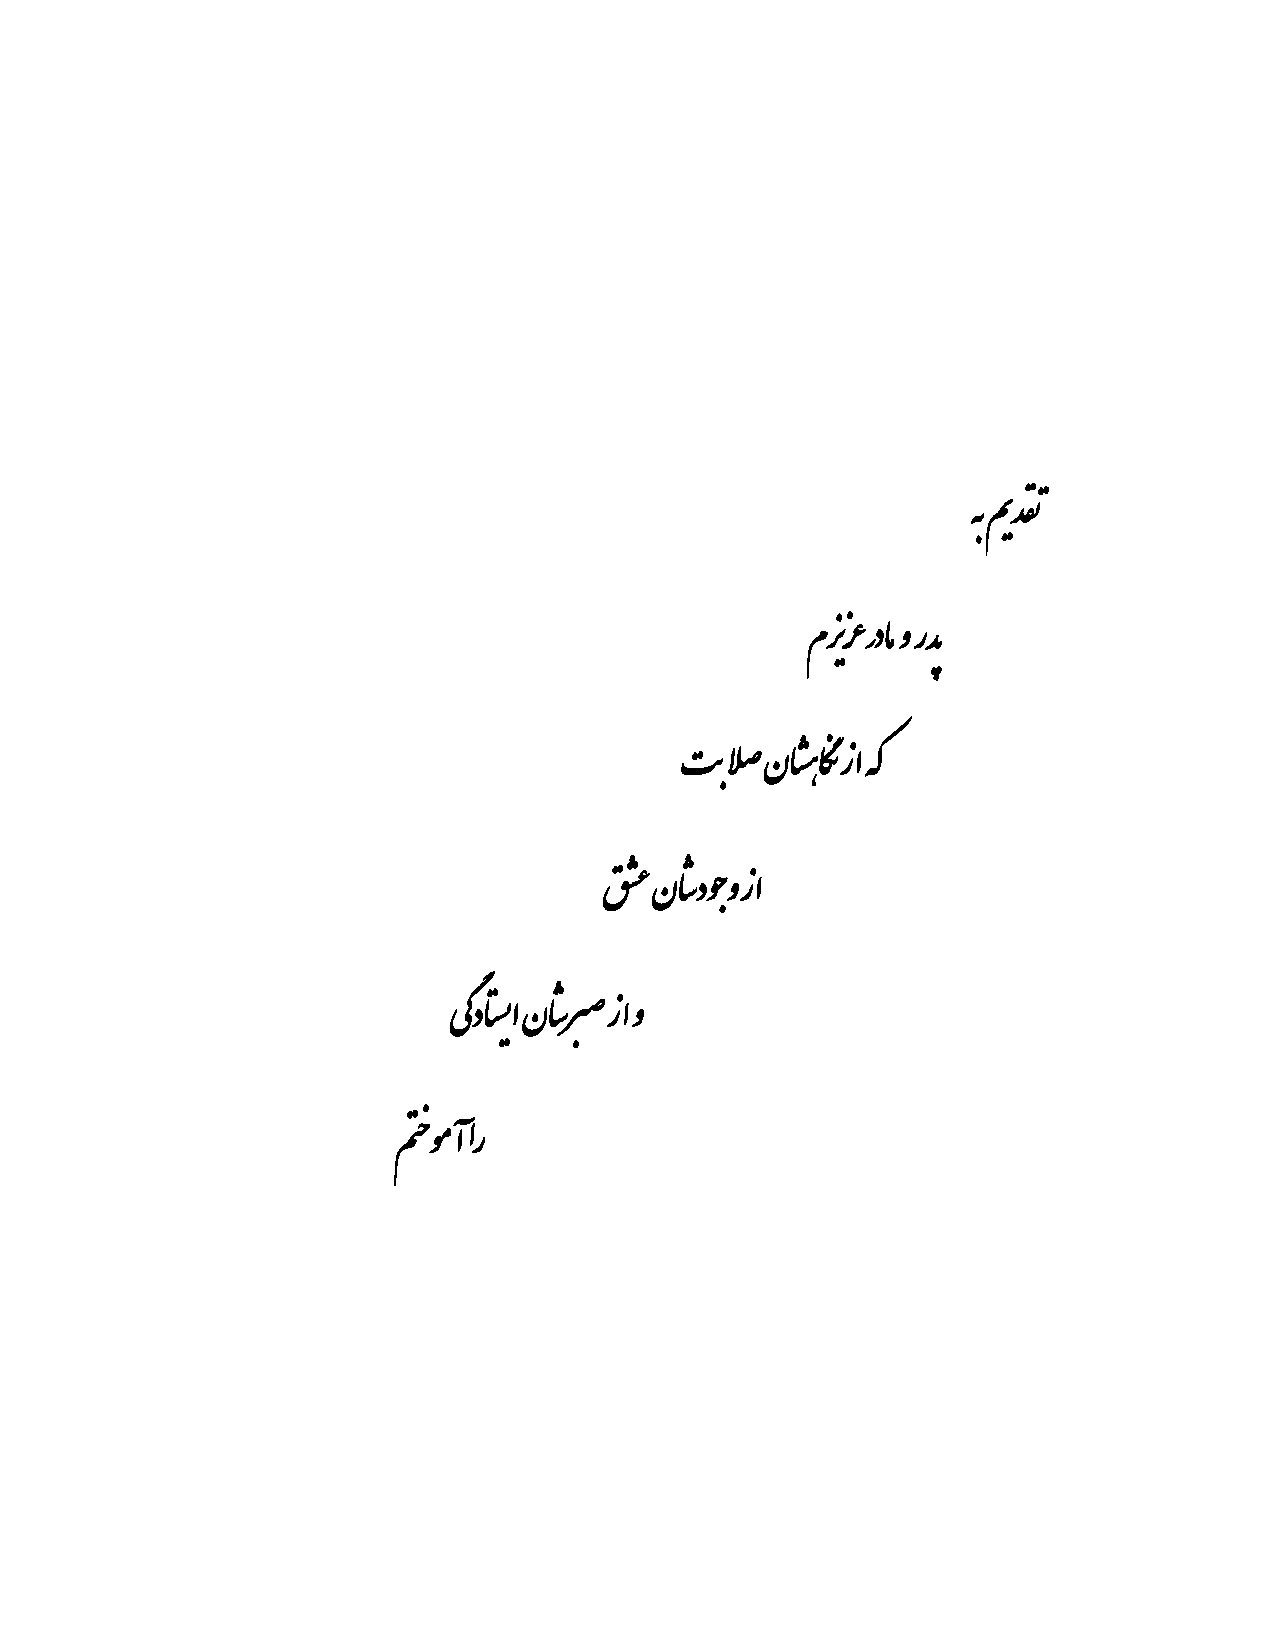
\includegraphics[scale=0.9]{Figures/taghdir.pdf} 


\newpage
\thispagestyle{empty}
\mbox{}


\newpage
\thispagestyle{empty}
{\nastaliqbig \Huge 
تقدیر و تشکر\nastaliq

{\par\vspace{1cm}}
\LARGE
\begin{adjustwidth}{1cm}{}
مراتب تشکر و قدردانی خود را نسبت به تمام کسانی که مرا در انجام این پایان‌نامه یاری کرده‌اند، خصوصاً استاد گرامی و ارجمندم، سرکار خانم دکتر شاکری که رهنمودهای ایشان همواره راهگشای پیچیدگی‌های این پژوهش بوده است، ابراز می‌دارم. 

همچنین، از تمامی دوستانم در آزمایشگاه سیستم‌های هوشمند اطلاعات که با حضور و محبتشان مرا یاری نمودند تشکر و قدردانی می‌نمایم. 

\end{adjustwidth}
}


\newpage
\thispagestyle{empty}
\mbox{}


\pagestyle{plain}

\newpage

\begin{center}
\vspace*{-2.6cm}
\subsection*{چکیده}
\end{center}
\vspace*{-.4cm}

\begin{spacing}{1.8}
با توجه به رشد روز‌‌افزون اطلاعات موجود در وب، موتورهای جست‌و‌جو در بازیابی اطلاعات مورد نیاز کاربران از میان حجم زیادی از اطلاعات نقشی اساسی ایفا می‌کنند. با بررسی رفتار کاربر در اینترنت مشاهده شده است که بیشترین بازدید از یک صفحه وب، به واسطه نتایج اولیه بازیابی شده توسط موتورهای جست‌و‌جو می‌باشد. با توجه به این امر، ایده هرزنویسی در وب با هدف افزایش رتبه صفحات هرز در میان نتایج موتورهای جست‌و‌جو مطرح شد. برای شناسایی و مقابله با این صفحات روش‌هایی ارائه شده است که می‌توان آن‌ها را به سه دسته کلی روش‌های مبتنی بر محتوا، روش‌های مبتنی بر پیوند و روش‌های مبتنی بر داده‌های جانبی تقسیم نمود. در این پژوهش تمرکز بر روی دو روش اصلی مبتنی بر محتوا و مبتنی بر پیوند و همچنین ترکیب این دو روش به منظور شناسایی وب‌گاه‌های هرز می‌باشد.

از آن‌جایی که عملکرد موتورهای جست‌و‌جو در شناسایی وب‌گاه‌های هرز فارسی پایین می‌باشد، در این پژوهش پس از ساخت یک مجموعه داد‌ه‌ای مناسب شامل وب‌گاه‌های هرز و معتبر فارسی، به بررسی و تحلیل تعدادی از ویژگی‌های محتوایی برای شناسایی وب‌گاه‌های هرز فارسی می‌پردازیم. سپس با ارائه چندین ویژگی محتوایی جدید و استفاده از روش‌های انتخاب ویژگی، کارایی رده‌بندی وب‌گاه‌ها را افزایش می‌دهیم. در ادامه، یک سامانه جدید شناساگر هرز وب فارسی را ارائه می‌دهیم که از مدل بهبود یافته کیف کلمات برای استخراج ویژگی‌ها استفاده می نماید و نسبت به روش‌های محتوایی پیشین کارایی بالاتری دارد. با توجه به گسترش استفاده از الگوریتم‌های مبتنی بر پیوند در روش‌های هرزنویسی، تعدادی از الگوریتم‌های مهم در این زمینه را مورد بررسی قرار داده و دو الگوریتم جدید ارائه می‌دهیم که بسیاری از نقاط ضعف الگوریتم‌های پیشین را ندارند. در الگوریتم اول برای بهبود انتشار امتیاز اعتماد در گراف وب، از سه سیاست انتخاب بهینه گره‌های بذر، وزن‌دهی به یال‌های گراف برای مشخص کردن میزان اعتبار یال‌ها، و بسط دوره‌ای گره‌های بذر استفاده می‌شود. در الگوریتم دوم با استفاده از انتشار امتیاز هرز، هم‌زمان به صورت پیش‌رو و پس‌رو در سراسر گراف وب، کیفیت رتبه‌بندی وب‌گاه‌های هرز را بهبود می‌دهیم.
در آخر نیز به منظور بهبود کیفیت رتبه‌بندی وب‌گاه‌ها روشی پیشنهاد داده می‌شود که برای انتشار امتیاز وب‌گاه‌ها، از احتمال اعتبار و هرز بودن محتوایی وب‌گاه‌ها در تمام بخش‌های گراف استفاده می‌نماید. 

در پایان این پژوهش، به منظور ارزیابی روش‌ها و بررسی میزان کارایی آن‌ها، آزمایش‌های مربوطه انجام شده است. نتایج آزمایش‌ها نشان می‌دهد که روش‌های ارائه شده در مقایسه با روش‌های قبلی، از کارایی و دقت بالاتری برخوردار هستند.
 
\textbf{واژه‌های کلیدی: }\textit{هرزنویسی، هرز وب، شناسایی هرز، انتشار برچسب، ویژگی‌های محتوایی.}
\end{spacing}

\pagenumbering{harfi}


\newpage
\thispagestyle{empty}
\mbox{}

\renewcommand\listfigurename{فهرست شکل‌ها}
\renewcommand\listtablename{فهرست جدول‌ها}
%\renewcommand{\refname}{مراجع}

\begin{doublespace}\small{
\tableofcontents
\listoftables
\listoffigures
}\end{doublespace}





\pagestyle{fancy}	
\fancyhead{} 
\fancyhead[RO]{\leftmark}
\fancyhead[LO]{\thepage}
\fancyhead[LE]{\rightmark}
\fancyhead[RE]{\thepage}
\fancyfoot{} 
\renewcommand{\headrulewidth}{0.6pt} 
\renewcommand{\footrulewidth}{0pt}

\chapter{مقدمه}
\label{chapter:introduction}
\pagenumbering{arabic}\setcounter{page}{1}
\thispagestyle{plain}
مفهوم \mls{هرز} به طور کلی برای هر \mls{سامانه} اطلاعاتی، که می‌تواند دارای ارزش محتوایی پایینی ‌باشد به‌کار می‌‌رود؛ مانند \mls{رایانامه}، \mls{وب‌نوشت}، وب و نظرهای کاربران در محیط‌های اجتماعی مجازی. در این میان، مفهوم \mls{هرز وب} برای اولین بار در سال ۱۹۹۶ مطرح شد  \cite{convey1996porn}. از آن پس تعاریف متعددی برای \mls{هرزنویسی وب} ارائه شد که در یک تعریف جامع  می‌توان آن را به  هرگونه عملیاتی نسبت داد که در میان نتایج بازیابی شده توسط \mls{موتورهای جست‌و‌جو} باعث افزایش امتیاز و \mls{رتبه} صفحات نامرتبط با \mls{پرس‌وجو} می‌شود \cite{gyongyi2005web}. همچنین در تعریفی دیگر که توسط \lr{Perkins}  ارائه شده است \cite{perkins2001classification}، هرزنویسی وب به هرگونه اقدامی گفته می‌شود که با هدف فریب الگوریتم‌های \mls{بازیابی اطلاعات} و الگوریتم‌های \mls{رتبه‌دهی} انجام می‌شود. یک صفحه یا \mls{وب‌گاه} هرز، صفحه یا وب‌گاهی است که دارای محتویات و خصوصیات خاصی می‌باشد که با هدف هرزنویسی ایجاد شده‌اند. این‌گونه از صفحات نه‌تنها اطلاعات مفیدی را در اختیار کاربران قرار نمی‌دهند، بلکه با کاهش کیفیت رتبه‌بندی نتایج پرس‌وجو‌ها، کاربران را از دسترسی به منابع اطلاعاتی مفید و مرتبط با پرس‌وجو محروم می‌نمایند.

با توجه به تاثیر صفحات هرز در کارایی موتورهای جست‌و‌جو، هرز وب پس از مدت کوتاهی به عنوان یکی از مسائل مهم در صنعت موتورهای جست‌و‌جو شناخته شد \cite{henzinger2002challenges}. همچنین، رشد سریع و روز‌ افزون وب، ساده بودن کار با ابزارهای ایجاد محتوا در وب (مانند ویکی‌پدیا، \mls{بسترهای نرم‌افزاری}، \mls{انجمن‌های گفتگو} و وب‌نوشت‌ها) و کاهش هزینه‌های نگهداری وب‌گاه‌ها موجب شده است که هرزنویسی در وب به سرعت افزایش پیدا کند و با گذشت زمان از روش‌های جدیدتری برای این منظور استفاده شود که با استفاده از راه‌حل‌های گذشته نتوان صفحات هرز را شناسایی کرد. با توجه به این مهم و همچنین اثرات نامطلوبی که صفحات هرز در کاهش کارایی موتورهای جست‌و‌جو و در نتیجه کاهش رضایت کاربران دارند، اخیرا تمام شرکت‌های طراح و پشتیبان موتورهای جست‌و‌جو، شناسایی  اطلاعات غیرمفید در وب  و مقابله با آن را به عنوان یکی از مسائل مهم در کار خود اعلام کرده‌اند \cite{fetterly2007adversarial}. این امر موجب شده است پژوهشگرانی که در این زمینه فعالیت می‌کنند به دنبال یافتن روش‌هایی جدید برای حل مشکلات ناشی از هرز وب باشند. 

از جمله مشکلاتی که هرز وب ایجاد می‌کند این است که صفحات هرز کیفیت نتایج جست‌و‌جو را پایین آورده و وب‌گاه‌های قانونی و معتبر را از امتیاز و سودی که در نبود صفحات هرز بدست می‌آورند محروم می‌کند. همچنین وجود این صفحات موجب می‌شود که اعتماد کاربران نسبت به توسعه‌دهنده یک موتور جست‌و‌جو کاهش یابد و  از موتور جست‌و‌جوی دیگری استفاده نمایند. از طرف دیگر، وجود هرز وب، شرکت‌های توسعه دهنده‌ موتورهای جست‌و‌جو را وادار می‌کند که هزینه‌های مالی و محاسباتی قابل توجهی را متحمل شوند. به‌علاوه، وب‌گاه‌های هرز با هدف ایجاد و انتشار  انواع \mls{بد‌افزار}‌ها و ویروس‌ها و ترویج محتویات و اطلاعات غیرمفید و نادرست ایجاد می‌شوند که برای کاربران اینترنت تهدیدی جدی محسوب می‌شود. در سال 2005، مجموع ضررهای مالی ناشی از وجود هرز وب حدود 50 میلیارد دلار \cite{jennings2005global} و این ضرر در سال 2009 برابر با 130 میلیارد دلار \cite{jennings2009cost} اعلام شده است. طی بررسی‌های جامعی که \lr{Ntoulas} و همکاران در سال 2006   \cite{Ntoulas:2006}   بر روی پیکره‌ بزرگی از صفحات وب انجام داده‌اند، مقدار هرز وب را برای زبان انگلیسی ٪۱۳/۸، زبان ژاپنی ٪۹، آلمانی ٪۲۲، و فرانسه ٪۲۵ گزارش کرده‌اند. آن‌ها همچنین نشان داده‌اند که ٪۷۰ از صفحات در \mls{دامنه} .biz و ٪۲۰ از صفحات در .com صفحات هرز می‌باشند.

از جمله دلایل اصلی پیدایش هرز وب را می‌توان تعداد محدود نتایج بازیابی شده توسط موتورهای جست‌و‌جو و نمایش نتایج بر اساس رتبه‌‌بندی دانست و این‌که کاربران معمولا فقط صفحاتی را بررسی می‌نمایند که در اوایل این فهرست نمایش داده می‌شوند. Silverstein و همکاران \cite{silverstein1999analysis} طی تحقیقاتی نشان داده‌اند که برای ۸۰ درصد از پرس‌وجو‌‌ها، کاربران فقط بر روی سه تا پنج نتیجه اول \mls{تلیک} می‌کنند. در تحقیقی دیگر، \lr{Jansen} و \lr{Spink} \cite{jansen2003analysis} نشان داده‌اند که حدود ۸۰ درصد از کاربرانی که از موتورهای جست‌و‌جو استفاده می‌کنند حداکثر سه صفحه اول نتایج بازیابی شده را بررسی می‌نمایند. بنابراین صفحاتی که بتوانند در فهرست صفحات بازیابی شده توسط موتورهای جست‌و‌جو رتبه بالاتری را بدست آورند، از این طریق ترافیک بیشتری را به سمت وب‌گاه خود هدایت می‌کنند. برای بسیاری از وب‌گاه‌های تجاری، افزایش تعداد کاربران بازدید‌کننده از وب‌گاه، به منزله افرایش تبلیغات، فروش و سایر سودهای تجاری می‌باشد. اگرچه سایت‌های معتبر برای افزایش مشتریان خود از روش‌های \mls{بهینه‌سازی موتور جست‌و‌جو} استفاده می‌کنند، اما در این میان \mls{هرزنویسان} با سوء ‌استفاده از این روش‌ها در صدد افزایش رتبه صفحه خود بیشتر از آن‌چه که استحقاقش را دارند هستند. آن‌ها برای رسیدن به این هدف از روش‌های مختلفی از جمله ایجاد تغییراتی در محتوای صفحه، ایجاد \mls{پیوند}های جعلی و تغییر مسیر به صفحه‌ای دیگر برای افزایش رتبه صفحات هرز خود استفاده می‌کنند. 

برای مقابله با انواع روش‌های هرزنویسی راه‌حل‌هایی ارائه شده است که می‌توان آن‌ها را بسته به نوع اطلاعاتی که استفاده می‌کنند در مجموع به سه دسته کلی روش‌های \mls{شناسایی} هرز وب مبتنی بر محتوا، مبتنی بر پیوند و مبتنی بر داده‌های پراکنده تقسیم نمود. در این پژوهش تمرکز ما بر روی دو روش اصلی مبتنی بر محتوا و مبتنی بر پیوند و همچنین ترکیب این دو روش می‌باشد. در ادامه انواع روش‌های مقابله با هرز وب را به طور مختصر معرفی می‌نماییم.
\subsubsection{روش‌های مبتنی بر محتوا}
روش‌های هرزنویسی مبتنی بر محتوا از جمله روش‌های اولیه و بسیار گسترده در زمینه هرزنویسی وب می‌باشند که اساس عملکرد آن‌ها ایجاد تغییراتی در محتوای صفحات وب است. با توجه به این‌که موتورهای جست‌و‌جو از مدل‌های مختلف بازیابی اطلاعات مبتنی بر محتوای صفحه مانند مدل \mls{فضای برداری} \cite{salton1975vector}، \lr{BM25} \cite{robertson2004simple} و \mls{مدل‌های زبانی آماری} \cite{zhai2008statistical} برای رتبه‌بندی صفحات استفاده می‌کنند، این روش‌ها با پیدا کردن نقاط ضعف این مدل‌ها موتورهای جست‌و‌جو را فریب داده و رتبه صفحات هرز را افزایش می‌دهند. بنابراین، در روش‌های مقابله با هرز مبتنی بر محتوا با بررسی \mls{ویژگی}‌های محتوایی صفحات و تحلیل و مقایسه \mls{مدل زبانی} آن‌ها میزان احتمال هرز بودن صفحات تخمین زده می‌شود.
 
بخش زیادی از الگوریتم‌هایی که در این روش‌ها استفاده می‌شوند الگوریتم‌های وابسته به زبان هستند و کارایی آن‌ها برای صفحات به زبان‌های مختلف، متفاوت می‌باشد. با وجود مطالعات زیادی که پیرامون کارایی روش‌های مبتنی بر محتوا بر روی صفحات وب انگلیسی انجام شده است، تا‌کنون هیچ مطالعه قابل توجهی بر روی شناسایی وب‌گاه‌های هرز فارسی صورت نگرفته است و موتورهای جست‌و‌جو نیز همچنان در شناسایی این نوع از صفحات هرز عملکرد پایینی دارند. این مهم در حالی است که \lr{Techs}‌$W^3$ \cite{W3Techs} میزان وب‌گاه‌های فارسی را در سال 2014 حدود ۰/۸ درصد تخمین زده ‌است که این مقدار به سرعت در حال افزایش می‌باشد. در نتیجه، بهبود دقت روش‌های شناسایی وب‌گاه‌های هرز فارسی می‌تواند تاثیر بسزایی در کارایی موتورهای جست‌و‌جو داشته باشد. همچنین به دلیل نبود پژوهشی قابل توجه در این زمینه، تاکنون هیچ \mls{مجموعه داده‌ای} \mls{برچسب} خورده‌ استانداردی از وب‌گاه‌های هرز فارسی ایجاد نشده است. بنابراین، در این پژوهش ابتدا به جمع‌آوری مجموعه‌ای از وب‌گاه‌های هرز فارسی پرداخته‌ایم و  وب‌گاه‌ها را به صورت دستی برچسب‌گذاری کرده‌ایم. توضیحات کامل‌ ساخت این مجموعه داده‌ای در بخش \ref{section:methodology-builddataset} ارائه شده است. 
پس از ساخت مجموعه‌ای از وب‌گاه‌های فارسی برچسب خورده، تاثیر انواع ویژگی‌های محتوایی و روش‌های مختلف \mls{یادگیری ماشین} بر روی شناسایی وب‌گاه‌های هرز فارسی بررسی شده و سپس تعدادی ویژگی محتوایی جدید برای شناسایی این نوع از وب‌گاه‌ها پیشنهاد شده است. برای بررسی میزان کارایی این ویژگی‌ها در شناسایی وب‌گاه‌های هرز فارسی، نمودار توزیع پراکندگی وب‌گاه‌ها و احتمال هرز بودن آن‌ها با توجه به مقادیر مختلف هر ویژگی به طور مجزا ارائه شده است.
در مرحله بعد با استفاده از روش‌ \mls{انتخاب ویژگی}‌ $\chi^2\text{-test}$ و روش \mls{حذف پس‌رو}، مجموعه‌ای از ویژگی‌ها به عنوان ویژگی‌های بهینه انتخاب شده‌اند. در نهایت وب‌گاه‌های موجود در مجموعه داده‌ای فارسی، با استفاده از مجموعه ویژگی‌های بهینه و الگوریتم \mls{جنگل تصادفی}  \mls{رده‌بندی}  شده‌اند. 
نتایج بخش ارزیابی نشان می‌دهد که کارایی ویژگی‌های محتوایی معرفی شده در این پژوهش با کارایی تعداد زیادی از ویژگی‌های محتوایی پیشین برابری می‌کند. به علاوه، هزینه محاسباتی ویژگی‌های جدید کمتر از بسیاری از ویژگی‌های محتوایی پیشین می‌باشد. همچنین بررسی نتایج حاصل از رده‌بندی وب‌گاه‌ها  پس از انتخاب مجموعه ویژگی‌های بهینه نشان می‌دهد که استفاده از تعداد ویژگی‌های بیشتر، نه‌تنها سبب بهبود نتایج رده‌بندی نمی‌شود، بلکه ترکیب برخی از این ویژگی‌های محتوایی با یکدیگر در مواردی کارایی رده‌بندی را کاهش می‌دهد. از طرف دیگر بررسی میزان تاثیر هر یک از ویژگی‌های محتوایی به تنهایی در کارایی رده‌بندی نشان می‌دهد که خصوصیات وب‌گاه‌های هرز به گونه‌ای می‌باشد که با استفاده از یک ویژگی محتوایی به تنهایی نمی‌توان تمام آن‌ها را شناسایی کرد.  

با توجه به این‌که با استفاده از مجموعه ویژگی‌های بهینه، همچنان امکان شناسایی تعدادی از وب‌گاه‌های هرز وجود ندارد، در ادامه با بررسی محتوای وب‌گاه‌های هرز و معتبر فارسی، یک سامانه جدید برای شناسایی هرز وب فارسی پیشنهاد شده است. در این سامانه از یک روش مبتنی بر مدل جدیدی به نام \mls{کیف کلمات هرز} (\lr{BOSW})  که نسخه‌ای تغییر یافته از مدل ساده \mls{کیف کلمات} می‌باشد، برای انتخاب ویژگی‌ها استفاده شده است. نتایج بخش ارزیابی نشان می‌دهد که این روش در تشخیص هرز وب فارسی از لحاظ دو معیار \mls{فراخوانی} و \mls{دقت} نسبت به روش‌های محتوایی پیشین بهتر عمل می‌کند.
\subsubsection{روش‌های مبتنی بر پیوند}
روش‌های هرزنویسی مبتنی بر پیوند، روش‌هایی هستند که در ساختار گرافی بین صفحات وب تغییراتی را ایجاد می‌کنند. این تغییرات به نحوی می‌باشند که در نهایت منجر به افزایش امتیازی می‌شوند که با استفاده از الگوریتم‌های رتبه‌بندی مبتنی بر گراف مانند \lr{PageRank} \cite{page1999pagerank}، \lr{HITS} \cite{kleinberg1999authoritative} و \lr{TrustRank} \cite{gyongyi2004combating} به صفحات داده می‌شود. یکی از این تغییرات ایجاد \mls{دهکده پیوندی} \cite{adali2005optimal, gyongyi2005link} می‌باشد. یک دهکده پیوندی مجموعه‌ای از صفحات وب است که با پیوند‌های زیادی به یکدیگر ارتباط دارند و می‌توانند با فریب الگوریتم‌های رتبه‌دهی امتیاز همه یا تعدادی از صفحات درون آن دهکده پیوندی را افزایش دهند. در سال ۲۰۰۰، \lr{Davision} \cite{davison2000recognizing} پس از ارائه تعریفی جامع برای هرزنویسی وب به روش مبتنی بر پیوند، روش‌هایی برای شناسایی پیوندهای جعلی در وب پیشنهاد داده است. طبق تعریف \lr{Davision}، هرزنویسی مبتنی بر پیوند به روش‌هایی گفته می‌شود که سعی در ایجاد پیوندهای جعلی بین صفحات دارند تا بدین طریق بتوانند رتبه پیوندی صفحات هرز را افزایش دهند. در این روش‌ها ساختار گرافی بین صفحات به نحوی تغییر داده می‌شود که با اعمال الگوریتم‌های رتبه‌بندی، صفحات هرز بتوانند رتبه‌ای بالاتر از آن چه که استحقاقش را دارند بدست آورند. 

با توجه به وجود این نوع از روش‌های هرزنویسی، به تدریج الگوریتم‌هایی برای مقابله با این نوع از صفحات هرز پیشنهاد داده شدند که اساس عملکرد آن‌ها بر روی ساختار کلی گراف و ارتباطات پیوندی بین صفحات است و از رو‌ش‌هایی برای انتشار امتیاز \mls{اعتماد} یا \mls{عدم اعتماد} صفحات، پیدا کردن دهکده‌های پیوندی، حذف پیوند‌های مشکوک و تشخیص رفتارهای غیرعادی در الگوریتم‌های رتبه‌بندی مبتنی بر پیوند استفاده می‌کنند. 

در این پژوهش، دو الگوریتم‌ مبتنی بر پیوند برای رده‌بندی وب‌گاه‌ها پیشنهاد شده است که اساس کار آن‌ها بر روش انتشار برچسب می‌باشد. در الگوریتم \lr{WorthyRank} با استفاده از روش‌هایی مانند انتخاب بهینه وب‌گاه‌های \mls{بذر}، بسط دوره‌ای مجموعه وب‌گاه‌های بذر و همچنین وزن‌دهی به  \mls{یال}‌های گراف وب و حذف یال‌های جعلی، دقت رتبه‌بندی صفحات وب بهبود داده می‌شود. در ادامه نیز الگوریتمی به نام \lr{JunkyRank} معرفی شده است که احتمال هرز بودن وب‌گاه‌ها را هم‌زمان به دو صورت \mls{پیش‌رو} و \mls{پس‌رو} در گراف وب انتشار می‌دهد. نتایج نشان می‌دهد که این الگوریتم در بازیابی و رتبه‌بندی صفحات هرز به نسبت روش‌های قبلی از دقت بالاتری برخوردار است. برای آزمایش روش‌های ارائه شده از دو مجموعه داده‌ای استاندارد \lr{WebSpamChallengeII-CorpusI} و \lr{WEBSPAM-UK2007} استفاده شده است. از دو معیار \mls{ضریب هرز} و \mls{ضریب اطمینان} نیز برای ارزیابی این روش‌ها استفاده شده است.

پس از معرفی و تحلیل هر یک از روش‌های مبتنی بر محتوا و مبتنی بر پیوند به طور مجزا، در آخر برای بهبود دقت و کارایی رتبه‌بندی وب‌گاه‌ها، روشی جدید ارائه شده است که از ترکیب  روش محتوایی با روش پیوندی استفاده می‌کند. در این روش ابتدا تعدادی از وب‌گاه‌ها به همراه مجموعه وب‌گاه‌های بذر گراف، به عنوان داده‌های آموزش انتخاب شده و برچسب‌گذاری می‌شوند. سپس با استفاده از ویژگی‌های محتوایی استخراج شده از این مجموعه وب‌گاه‌ها، یک \mls{رده‌بند} محتوایی ساخته می‌شود. در مرحله بعد با استفاده از این رده‌بند برای هر یک از وب‌گاه‌های گراف، احتمال اعتبار و هرز بودن محتوایی محاسبه می‌شود. در نهایت با استفاده از الگوریتم‌های پیوندی ارائه شده در این پژوهش و با در نظر گرفتن احتمال هرز و اعتبار محتوایی هر \mls{گره}، میزان اعتبار وب‌گاه‌های بذر در کل گراف انتشار داده می‌شود. با استفاده از این روش، برای هر وب‌گاه یک امتیاز نهایی اعتبار و یا عدم اعتبار محاسبه شده و وب‌گاه‌ها بر اساس این امتیاز نهایی رتبه‌بندی می‌شوند. نتایج بخش ارزیابی نشان می‌دهد که این روش نسبت به سایر روش‌های ارائه شده در این پژوهش از دقت بالاتری برخوردار است.

\subsubsection{روش‌های مبتنی بر داده‌های پراکنده}
این دسته از روش‌ها برای شناسایی صفحات هرز از اطلاعاتی استفاده می‌کنند که فراتر از محتویات \mls{ایستا}ی صفحات و یا ساختار گرافی آن‌ها می‌باشد. یکی از این روش‌ها بررسی و تحلیل رفتار کاربران در مرورگرهای اینترنتی می‌باشد. برای مثال سابقه جست‌وجوهای کاربران در محیط وب و بررسی تاریخچه تلیک بر روی پیوندهای مختلف می‌تواند اطلاعات خوبی را درباره میزان مفید بودن وب‌گاه‌های مختلف و ارتباط آن‌ها با یکدیگر در اختیار قرار دهد. تحلیل اطلاعات مربوط به \lr{HTTP} (\mls{در سمت سرویس‌گیرنده} و \mls{در سمت سرویس‌دهنده})، محاسبه مدت زمان استفاده کاربران از صفحات هر وب‌گاه و سایر اطلاعاتی که به طور \mls{برخط} توسط موتورهای جست‌و‌جو جمع‌آوری و به‌روز می‌شود،  روش‌های خوبی برای تخمین میزان اعتبار وب‌گاه‌های مختلف هستند. با توجه به این‌که موتورهای جست‌و‌جو امکان دسترسی به این اطلاعات را برای کاربران عادی فراهم نمی‌کنند، در این پژوهش از بررسی این دسته از روش‌ها صرف‌نظر شده است.

در ادامه این نوشتار، در فصل \ref{chapter:relatedWork}، تعدادی از کارهای پیشین مرتبط با انواع روش‌های شناسایی و مقابله با هرز وب را مرور می‌نماییم. شرح کامل انواع روش‌های پیشنهادی برای رده‌بندی وب‌گاه‌ها در فصل \ref{chapter:methodology} ارائه می‌شود. در این فصل ابتدا انواع ویژگی‌های محتوایی را که برای رده‌بندی وب‌گاه‌های فارسی استفاده کرده‌ایم توضیح داده و تعدادی ویژگی محتوایی جدید را معرفی می‌نماییم. همچنین روش محتوایی دیگری را معرفی می‌کنیم که از مدل کیف کلمات هرز برای استخراج ویژگی‌های محتوایی استفاده می‌کند. در ادامه این فصل، دو الگوریتم مبتنی بر پیوند و \mls{نیمه‌سرپرست} را معرفی می‌کنیم که به نسبت روش‌های قبلی کارایی و دقت بالاتری دارند. در نهایت نیز الگوریتمی را پیشنهاد می‌دهیم که از ترکیب  روش محتوایی با روش‌های پیوندی برای رتبه‌بندی وب‌گاه‌ها استفاده می‌کند. در فصل \ref{chapter:experiments} ابتدا توضیحاتی را درباره مجموعه داده‌ای‌های استفاده شده در این پژوهش ارائه می‌دهیم، سپس پس از معرفی معیارهای ارزیابی، تمام روش‌های معرفی شده در این پژوهش را مورد آزمایش و ارزیابی قرار می‌دهیم. همچنین تحلیل‌های مربوط به نتایج هر آزمایش نیز در این فصل بیان شده است. در نهایت در فصل \ref{chapter:conclusion}، ضمن جمع‌بندی مطالب و نتیجه‌گیری، پیشنهادهایی برای کارهای آینده در این زمینه ارائه می‌دهیم.

%%%%%%%%%%%%%%%%%%%%%%%%%%%%%%%%%%%%%%%%%%%%%%%%%%%%%%
%\newpage
%\thispagestyle{empty}
%\mbox{}

\chapter{پژوهش‌های پیشین}
\label{chapter:relatedWork}
\thispagestyle{plain}
در این فصل، روش‌هایی که تاکنون برای هرزنویسی وب و همچنین تشخیص صفحات هرز معرفی شده‌اند را در چهار گروه اصلی دسته‌بندی و بررسی می‌کنیم. بدین منظور، ابتدا به مطالعه روش‌های مبتنی بر محتوا می‌پردازیم، سپس مطالعات انجام شده بر روی روش‌های مبتنی بر پیوند را بررسی می‌نماییم. در بخش بعد، کارهایی را مرور می‌کنیم که از اطلاعات مربوط به رفتار کاربران در محیط وب برای شناسایی صفحات هرز استفاده می‌کنند. در آخر نیز تعدادی از پژوهش‌های اخیر را که از ترکیب روش‌های قبلی استفاده می‌کنند، مورد مطالعه قرار می‌دهیم.

\section{روش‌های مبتنی بر محتوا}
\label{section:relatedwork-content}
از جمله فعالیت‌هایی که در رابطه با تشخیص صفحات وب هرز بر مبنای محتوای صفحات صورت گرفته است، تحقیقات انجام شده توسط \lr{Fetterly} و همکاران \cite{Fetterly:2004, Fetterly:2003, Fetterly:2005, fetterly2007adversarial} است. آن‌ها در پژوهشی \cite{Fetterly:2004} در سال 2004، نشان داده‌اند که استفاده از تحلیل‌های آماری در شناسایی انواع صفحات وب هرز به خصوص صفحاتی که به طور خودکار توسط ماشین ایجاد شده‌اند بسیار کاربرد دارد. بدین منظور، تعدادی ویژگی برای شناسایی صفحات هرز معرفی کرده‌اند که عبارتند از: تعداد پیوندهای ورودی به هر صفحه، تعداد پیوندهای خروجی، تعداد کلمات \mls{غیر‌نشانه‌گذاری} هر صفحه، میزان شباهت محتوای صفحات که با استفاده از الگوریتم \lr{Shingling} \cite{Broder:1997} محاسبه شده و \mls{خوشه‌بندی} آن‌ها، ویژگی‌های خاص مربوط به آدرس اینترنتی صفحات، بررسی آدرس IP مربوط به هر \mls{نام میزبان}، و سرعت و درصد تغییر محتوای صفحات در طول زمان \cite{Fetterly:2003}. سپس با انجام آزمایش‌هایی نشان داده‌اند که به ازای هر یک از ویژگی‌های تعریف شده، داده‌های با مقادیر \mls{برون‌هشته}‌‌ با احتمال زیادی نمایان‌گر صفحات هرز می‌باشند. نتایج آزمایش بر روی آدرس اینترنتی صفحات نشان می‌دهد که آدرس صفحات هرز معمولا دارای تعداد زیادی کلمه، نقطه، خط تیره و عدد می‌باشد. همچنین با بررسی آدرس \lr{IP} و نام میزبان صفحات نشان داده‌اند که چندین وب‌گاه هرز با نام میزبان متفاوت، دارای یک آدرس \lr{IP} مشترک هستند. خصوصیت دیگری که در این مقاله به عنوان یکی از ویژگی‌های صفحات هرز بیان شده است، سرعت زیاد و درصد بالای تغییرات محتوای ایستای صفحات می‌باشد.

در پژوهشی دیگر، \lr{Fetterly} و همکاران \cite{Fetterly:2005} روشی را معرفی کرده‌اند که می‌تواند دسته‌ای از صفحات هرز را شناسایی کند که دارای محتوای تکراری در سطح عبارت هستند. محتوای این صفحات با کنار هم گذاشتن بخش‌هایی از محتوای صفحات دیگر ساخته می‌شود. روشی که در این پژوهش برای شناسایی این دسته از صفحات استفاده شده است، از بسیاری از ویژگی‌های روش \mls{انگشت‌نگاری} Robin \cite{Broder:1993,Rabin:1981} بهره می‌گیرد. در سال 2006، در راستای تکمیل کارهای قبلی \cite{Fetterly:2004, Fetterly:2005}، \lr{Ntoulas} و همکاران \cite{Ntoulas:2006} تعدادی ویژگی محتوایی را برای شناسایی خودکار صفحات  هرز معرفی کرده و میزان کارایی هر یک را به طور مجزا در تشخیص این نوع از صفحات بررسی کرده‌اند. سپس، با ترکیب ویژگی‌ها و استفاده از روش‌های مختلف یادگیری ماشین، دقت رده‌بندی را افزایش داده‌اند. نتایج آن‌ها نشان می‌دهد که بالاترین میزان دقت رده‌بندی برای الگوریتم \mls{درخت تصمیم} است که توانسته‌اند با استفاده از دو روش \lr{bagging} \cite{Breiman:1996} و \lr{boosting} \cite{Freund:1995} دقت این الگوریتم را نیز افزایش دهند. در هر دو روش مجموعه‌ای از رده‌بند‌ها ایجاد و در نهایت با یکدیگر ترکیب می‌شوند تا یک رده‌بند با دقت بالاتر ایجاد کنند. هفت سال بعد، Prieto و همکاران \cite{Prieto:2013} یک سامانه شناسایی و تحلیل هرز به نام \lr{SAAD} معرفی کرده‌اند که بر مبنای تعدادی ویژگی محتوایی کار می‌کند. در این سامانه علاوه بر استخراج ویژگی‌های محتوایی معرفی شده در مقاله \cite{Ntoulas:2006}، تعدادی ویژگی محتوایی جدید نیز معرفی و استخراج شده است. این ویژگی‌ها عبارتند از: متوسط طول لغات (با حذف \mls{ایست‌واژه}‌ها و \mls{ابربرچسب}‌ها)، درصد کد \mls{پویا} و ایستای موجود در صفحه، تعداد عکس‌های بدون توضیح و برچسب، تعداد ایست‌واژه‌ها و تعدادی ویژگی دیگر. در این مقاله نیز پس از تحلیل کارایی هر یک از ویژگی‌های ارائه شده به طور مجزا، با ترکیب این ویژگی‌ها و ویژگی‌های معرفی شده در مقاله \cite{Ntoulas:2006} و استفاده از الگوریتم درخت تصمیم به همراه دو روش \lr{bagging} و \lr{boosting} به دقت بالاتری رسیده‌اند. 

\lr{Sydow} و همکاران \cite{Sydow:2007}، کاربرد انواع روش‌های یادگیری ماشین را در شناسایی صفحات وب هرز بررسی کرده‌اند. بدین منظور آن‌ها از تعدادی ویژگی زبانی استفاده کرده و میزان کارایی آن‌ها را در شناسایی صفحات هرز مورد بررسی قرار داده‌اند. در یک پژوهش کامل‌تر، \lr{Piskorski} و همکاران \cite{Piskorski:2008} برای بهبود شناسایی صفحات هرز تعدادی ویژگی زبانی جدید پیشنهاد داده‌اند. بسیاری از این ویژگی‌های زبانی که شامل تعداد کلمات متمایز موجود در متن صفحه، تعداد اسم‌ها و فعل‌ها، تعداد جملات مجهول، میزان \mls{گوناگونی} در لغات و محتوای متن و میزان نقل قول‌های مستقیم و غیرمستقیم می‌باشند با استفاده از ابزارهای \mls{پردازش زبان طبیعی} استخراج شده‌اند.
\lr{Martinez-Romo} و همکاران \cite{martinez2009web}، با بهره‌گیری از مدل‌ زبانی صفحات و محاسبه میزان اختلاف آن‌ها، صفحات وب هرز را شناسایی می‌کنند. این روش قبلا در کاربردهای بسیاری مانند شناسایی و مقابله با وب‌نوشت‌های هرز \cite{mishne2005blocking} استفاده شده است. با بهره‌گیری از این روش، در مقاله \cite{martinez2009web}، مدل زبانی\mls{متن پیوند}  و کلمات موجود در آدرس الکترونیکی صفحه مبدا با مدل زبانی عنوان و بدنه صفحه مقصد مقایسه شده و اختلاف \lr{Kullback-Leibler (KL) Divergence} بین این دو مدل زبانی محاسبه می‌شود. در صورتی ‌که میزان این اختلاف از یک آستانه مشخص بیشتر باشد صفحه مقصد با احتمال بالایی هرز است. از جمله مزیت‌های این روش این است که نیازی به \mls{داده‌های آموزش} نداشته و هزینه و زمان اجرای کمتری دارد.
برخلاف بسیاری از کارهای قبلی که از محتویات غیر‌نشانه‌گذاری صفحات برای تشخیص هرز بودن یا نبودن آن‌ها استفاده کرده‌اند، Urvoy و همکاران \cite{urvoy2006tracking}، از ویژگی‌های مبتنی بر ساختار صفحات \lr{HTML} برای رده‌بندی صفحات وب استفاده می‌کنند. در این روش‌ها، طی یک مرحله پیش‌پردازش تمامی محتویات قابل مشاهده صفحات حذف شده و قالب اصلی صفحه \lr{HTML} نگه داشته می‌شود. سپس برای پیدا کردن گروه‌هایی از صفحات که از لحاظ ساختار صفحه مشابه یکدیگر می‌باشند از روش‌ انگشت‌نگاری \cite{Broder:1993,Rabin:1981} صفحات و سپس خوشه‌بندی آن‌ها استفاده می‌کنند. 

در دسته دیگری از کارها \cite{Biro:2008,pavlov2011detecting,dong2012effectively,suhara2013automatically}، از روش \mls{مدل موضوعی} برای شناسایی صفحات وب هرز استفاده می‌شود. مدل موضوعی یک مدل آماری است که مشخص می‌کند یک سند یا مجموعه‌ای از اسناد در رابطه با چه موضوع یا موضوعاتی می‌باشد. یکی از ساده‌ترین روش‌های ایجاد مدل موضوعی، روش \lr{Latent Dirichlet Allocation} (\lr{LDA}) \cite{blei2003latent} می‌باشد که با استفاده از آن می‌توان برای هر سند مجموعه‌ای از موضوعات مرتبط با آن سند به همراه احتمال مربوط بودن هر یک به آن سند را مشخص کرد. \lr{Biro} و همکاران \cite{Biro:2008}، از \lr{LDA} برای شناسایی هرز وب استفاده می‌کنند. آن‌ها برای هر وب‌گاه، یک سند به صورت کیف کلمات ایجاد کرده و الگوریتم LDA را بر روی هر دسته از صفحات هرز و معتبر اجرا می‌کنند. با این روش، در مرحله آموزش مجموعه‌ای از موضوع‌های هرز و معتبر ایجاد می‌شود. در مرحله آزمون، برای هر صفحه مدل موضوعی آن را ایجاد کرده و در صورتی ‌که احتمال موضوعی هرز آن از یک میزان مشخصی بالاتر باشد آن صفحه به عنوان صفحه هرز شناسایی می‌شود. در پژوهشی دیگر \cite{pavlov2011detecting}، از توزیع احتمال موضوعی در کنار تحلیل گوناگونی در سطح حروف، کلمات و جملات برای شناسایی هرز وب استفاده می‌شود. با استفاده از این روش، صفحاتی که دارای مدل موضوعی با توزیع احتمال یکنواخت هستند به احتمال زیاد صفحات معتبر می‌باشند و به میزانی که این توزیع از یکنواخت بودن فاصله می‌گیرد احتمال هرز بودن صفحات افزایش می‌یابد. در سال 2012 نیز \lr{Dong} و \lr{Zhou} \cite{dong2012effectively}، با معرفی تعدادی معیار گوناگونی موضوعی، پژوهشی مشابه \cite{pavlov2011detecting} را انجام داده‌اند. Suhara و همکاران \cite{suhara2013automatically}، با بهره‌گیری از روشی که در \cite{riedl2012sweeping} ارائه شده است، به‌جای ایجاد مدل موضوعی از روی کل یک سند، هر جمله را یک سند مجزا در نظر گرفته و برای آن یک مدل موضوعی ایجاد می‌کنند. تفاوتی که کار آن‌ها با کار قبلی دارد این است که به‌جای استفاده از توزیع احتمال موضوعی، هر جمله را با موضوعی که بالاترین احتمال را دارد جایگزین می‌کنند. بدین ترتیب، هر سند را به دنباله‌ای از موضوعات تبدیل کرده و سپس میزان گوناگونی موضوعی داخل هر صفحه را بررسی می‌کنند. سپس با انجام آزمایش‌هایی نشان می‌دهند که میزان بی‌نظمی موضوعی در صفحات هرز بیشتر است.

در سال‌های اخیر، مطالعات زیادی در زمینه شناسایی صفحات وب هرز عربی انجام شده ‌است. بدین منظور، \lr{Wahsheh} و همکاران \cite{wahsheh2011detecting} مجموعه‌ای از صفحات وب عربی را تهیه کرده‌ و به صورت دستی برچسب‌گذاری کرده‌اند. در پژوهش‌های دیگر \cite{jaramh2011detecting,al2011combating} کارایی برخی از ویژگی‌های محتوایی بر روی این مجموعه صفحات وب عربی، بررسی شده است. سپس با استفاده از الگوریتم‌های یادگیری ماشین، نشان داده‌اند که درخت تصمیم بالاترین میزان دقت را در شناسایی هرز وب عربی دارد. در سال 2012، \lr{Al-Kabi} و همکاران \cite{al2012content}، مجموعه‌ای کامل‌تر از صفحات وب هرز عربی را جمع‌آوری و برچسب‌گذاری کرده‌اند. سپس با استفاده از روش‌های محتوایی و الگوریتم‌های یادگیری ماشین صفحات را رده‌بندی کرده‌اند. \lr{Al-Kabi} و همکاران \cite{al2014olawsds} در آخرین پژوهش خود در سال 2014، با معرفی یک سامانه بر‌خط شناسایی هرز وب عربی که از هر دو ویژگی محتوایی و پیوندی و همچنین از اطلاعات مربوط به بازخوردهای کاربران استفاده می‌کند، توانسته‌اند دقت تشخیص هرز وب عربی را افزایش دهند.
\section{روش‌های مبتنی بر پیوند}
\label{section:relatedwork-link}
با توجه به مطالعاتی که در راستای انجام این پژوهش، بر روی روش‌های مبتنی بر پیوند صورت گرفته است، این گروه از روش‌ها را می‌توان به سه دسته اصلی تقسیم کرد. دسته اول پژوهش‌هایی \cite{amitay2003connectivity, becchetti2006link, drost2005thwarting} هستند که ابتدا تمام ویژگی‌های پیوندی صفحات را استخراج کرده، سپس از الگوریتم‌های یادگیری ماشین برای رده‌بندی صفحات استفاده می‌کنند. دومین دسته از این روش‌ها، الگوریتم‌هایی \cite{wu2005identifying, wu2006undue, lempel2000stochastic} هستند که از ایده بهینه‌سازی برچسب‌ها بر اساس ساختار گرافی وب و همچنین روش‌های \lr{graph regularization}  \cite{abernethy2010graph, cheng2011let, zhou2007transductive} برای تشخیص صفحات هرز استفاده می‌کنند. الگوریتم‌های دسته سوم\cite{castillo2007know, page1999pagerank, caverlee2007countering, joshi2007anchor, gan2007improving, baeza2006generalizing}، ارتباطات ساختاری (مانند فاصله صفحات در گراف وب، ارجاع‌های مشترک، شباهت) بین صفحات برچسب‌دار و سایر صفحات در گراف وب را بررسی کرده و از میزان و نحوه ارتباط آن‌ها با یکدیگر برای رده‌بندی صفحات استفاده می‌کنند. در تعدادی از این روش‌ها \cite{gyongyi2004combating, krishnan2006web, wu2006propagating, becchetti2006using, geng2009link}، با داشتن برچسب تعدادی از صفحات بذر و همچنین روش انتشار برچسب، میزان هرز بودن یا نبودن سایر صفحات  محاسبه می‌شود. با توجه به این‌که تمرکز اصلی ما در این پژوهش بر روی این دسته از روش‌های مبتنی بر پیوند می‌باشد، در ادامه توضیحات بیشتری را پیرامون این الگوریتم‌ها ارائه می‌دهیم.

ایده اصلی در این دسته از الگوریتم‌های نیمه‌سرپرست این است که با داشتن برچسب مجموعه‌ای از گره‌های گراف (صفحات وب) و با استفاده از قوانین انتشار مختلف، سعی می‌کنند تا برچسب سایر صفحات را پیش‌بینی کنند. یکی از کارهای اولیه در این زمینه الگوریتم \lr{TrustRank} \cite{gyongyi2004combating} است که بر اساس این فرضیه ارائه شده است که صفحات معتبر معمولا به صفحات معتبر ارجاع می‌دهند. در این روش، مجموعه‌ای از صفحات معتبر به عنوان گره‌های بذر انتخاب شده و امتیاز اعتماد از طریق پیوندهای خروجی و با استفاده از الگوریتم \lr{PageRank} \mls{شخصی‌سازی شده} از این مجموعه صفحات معتبر به سایر مجموعه صفحات گراف انتشار داده می‌شود. \lr{Gyongyi} و همکاران \cite{gyongyi2004combating} نشان داده‌اند که در تشخیص صفات وب هرز، الگوریتم \lr{TrustRank} نسبت به الگوریتم \lr{PageRank} دقت و کارایی بیشتری دارد. در سال ۲۰۰۶، \lr{Wu} و همکاران \cite{wu2006topical} الگوریتم \lr{TrustRank} \mls{موضوعی} را پیشنهاد داده‌اند که صفحات بذر را بر اساس موضوعشان دسته‌بندی می‌کنند. سپس الگوریتم \lr{TrustRank} برای هر موضوع به طور جداگانه اجرا می‌شود. در نهایت با ترکیب این امتیاز‌ها، میزان اعتبار نهایی صفحات  مشخص می‌شود. در پژوهشی دیگر \cite{caverlee2007countering} برای بهبود الگوریتم \lr{TrustRank}، روشی پیشنهاد شده است که کیفیت پیوندهای یک صفحه را مستقل از کیفیت خود صفحه در نظر گرفته است و هدف آن تخصیص امتیاز پیوندی به هر صفحه بر اساس کیفیت پیوندهای آن می‌باشد. همچنین \lr{Chen} و همکاران \cite{chen2008link} با بررسی پیوندهای متغیر و میزان تغییرات در ساختار پیوندی گراف بین صفحات، توانسته‌اند الگوریتم \lr{TrustRank} را بهبود دهند. روش دیگر، الگوریتم  \lr{Anti-TrustRank} \cite{krishnan2006web} است که امتیاز هرز بودن را از مجموعه‌ای از صفحات هرز اولیه به سایر صفحات انتشار می‌دهد. نحوه انتشار امتیاز هرز در این الگوریتم مانند الگوریتم \lr{TrustRank} است. با این تفاوت که برای اجرای این الگوریتم، امتیاز هرز بودن مجموعه صفحات بذر، در خلاف جهت یال‌های گراف به سایر صفحات انتشار داده می‌شود. این امر به این دلیل است که اساس این الگوریتم بر اساس این فرضیه است که صفحاتی که به صفحات هرز ارجاع می‌دهند با احتمال زیادی هرز هستند. \lr{Krishnan} و همکاران \cite{krishnan2006web} نشان داده‌اند که الگوریتم \lr{Anti-TrustRank} نسبت به الگوریتم \lr{TrustRank} دقت بالاتری دارد و توانایی آن نیز در تشخیص صفحات هرزی که \lr{PageRank} بالاتری دارند بیشتر است.
 
  \lr{Wu} و همکاران \cite{wu2005identifying} روشی را ارائه داده‌اند که می‌تواند صفحات هرز درون دهکده‌های پیوندی را تشخیص دهد. در این روش ابتدا برای انتخاب مجموعه صفحات بذر، به ازای هر صفحه، تعداد صفحات مشترک بین صفحاتی که به آن صفحه ارجاع داده‌اند و صفحاتی که توسط آن صفحه ارجاع داده شده‌اند محاسبه می‌شود. سپس  در صورتی ‌که این تعداد، از یک آستانه مشخص بیشتر باشد، آن صفحه به عنوان صفحه بذر انتخاب می‌شود. این روش انتخاب بذر بر اساس ارتباط زیاد صفحات درون دهکده پیوندی تعریف شده است. سپس با توجه به این امر که اگر صفحه هرزی به تعداد زیادی صفحه هرز پیوند داده باشد، با احتمال زیادی خود یک صفحه هرز است، در هر مرحله صفحاتی  که تعداد ارجاعاتشان به صفحات بذر بیشتر از آستانه تعریف شده باشد، به مجموعه صفحات بذر اضافه می‌شوند. این الگوریتم تا جایی ادامه پیدا می‌کند که از آن پس، صفحه جدیدی به عنوان صفحه هرز شناسایی نشود. 

پس از معرفی روش‌های نیمه‌سرپرست انتشار برچسب که به مجموعه‌ای از صفحات برچسب خورده به عنوان صفحات بذر الگوریتم نیاز دارد، پژوهش‌هایی در رابطه با چگونگی انتخاب بذر اولیه و تاثیراتی که بر کارایی نهایی الگوریتم دارد انجام شد. \lr{Jiang} و همکاران \cite{jiang2008larger} نشان داده‌اند که در صورتی ‌که اندازه بذر در الگوریتم‌های انتشار برچسب مانند الگوریتم \lr{TrustRank} کم باشد، نتیجه نهایی به سمت صفحات بذر \mls{سوگیری} می‌کند. کم بودن تعداد صفحات بذر اولیه باعث می‌شود که درصد بیشتری از امتیاز صفحات، به صفحات بذر اختصاص یابد و در نتیجه در نتایج نهایی با احتمال زیادی این صفحات در رتبه‌های بالاتر قرار بگیرند. آن‌ها پیشنهاد داده‌اند که تعداد صفحات بذر باید با توجه به این‌که چند نتیجه اول برای کاربر مهم است، انتخاب شود. بدین صورت که در شرایطی که کاربر تعداد نتایج بیشتری را بررسی می‌کند، تعداد صفحات بذر اولیه نیز باید بیشتر باشد. از طرف دیگر افزایش اندازه بذر اولیه، هزینه زمانی را افزایش می‌دهد. با توجه به این مهم، \lr{Zhang} و همکاران \cite{zhang2009automatic} یک روش خودکار برای افزایش تعداد صفحات بذر اولیه پیشنهاد داده‌اند. در این الگوریتم که به صورت دوره‌ای تکرار می‌شود، با داشتن مجموعه صفحات معتبر اولیه، در هر تکرار، تمام صفحاتی که به هر صفحه پیوند داده‌اند بررسی شده و در صورتی که در این میان تعداد صفحات معتبر از مقدار آستانه بیشتر باشد، صفحه مبدا به عنوان صفحه معتبر شناخته شده و به بذر اولیه اضافه می‌شود. شرط بیشتر بودن از آستانه به این دلیل است که با پیدایش وب‌نوشت‌ها و \mls{انجمن}‌های مختلف که امکان نوشتن نظرات و مطالب گوناگون را به کاربرهای مختلف می‌دهند، هرز‌نویسان با قرار دادن پیوند صفحه هرز خود در این بخش از صفحات معتبر، سعی در فریب روش‌های پیوندی دارند. بدین ترتیب، اگرچه ممکن است صفحات هرز با استفاده از چنین روش‌هایی \cite{gyongyi2006link} تعدادی پیوند از صفحات معتبر به صفحات خود ایجاد کنند، اما به دلایلی از جمله مشکل هزینه و زما‌ن‌بر بودن این کار، امکان ایجاد چنین پیوندهایی به تعداد زیاد وجود ندارد. در \cite{wu2006topical} نیز  \lr{Wu} و همکاران، مرحله انتخاب بذر را به عنوان مهم‌ترین بخش الگوریتم \lr{TrustRank} دانسته‌اند و معتقدند که چگونگی انتخاب بذر اولیه در کارایی نهایی الگوریتم تاثیر می‌گذارد. آن‌ها با در نظر گرفتن این امر که صفحات وب در رابطه با موضوعات مختلفی هستند، نشان داده‌اند که نتایج نهایی روش \lr{TrustRank} به سمت صفحاتی سوگیری می‌شود که موضوعشان با موضوع صفحات بذر یکسان است. برای جلوگیری از این مشکل، صفحات بذر را از موضوعات مختلف انتخاب کرده و آن‌ها را بر اساس موضوعشان به گروه‌های مختلف تقسیم می‌کنند. سپس الگوریتم انتشار برچسب را برای هر گروه با موضوع مجزا اجرا کرده و امتیاز نهایی صفحات را از ترکیب امتیازهایی که برای هر موضوع بدست آورده‌اند، محاسبه می‌کنند. \lr{Zhao} و همکاران \cite{zhao2008good} نشان داده‌اند که در انتخاب بذر اولیه، استفاده از صفحات هرز با تعداد پیوندهای ورودی بیشتر، کارایی الگوریتم‌  \lr{Anti-TrustRank} را افزایش می‌دهد. در سال 2009، \lr{Zhang} و همکاران \cite{zhang2009exploiting, zhang2009deeply} برای محاسبه اعتبار صفحات، الگوریتمی به نام \lr{CPV} معرفی کرده‌اند که اساس روش آن مبتنی بر الگوریتم \lr{HITS} \cite{kleinberg1999authoritative} می‌باشد و از پیوندهای \mls{دوجهته} برای بهبود امتیازدهی به صفحات استفاده می‌کند. در این الگوریتم نیز مانند \lr{HITS} در هر تکرار الگوریتم، دو امتیاز مبتنی بر \lr{hub} و \lr{authority} به ترتیب به نام‌های \lr{HVRank} و \lr{AVRank} برای هر صفحه محاسبه شده و در نهایت از ترکیب این دو امتیاز برای محاسبه میزان اعتبار صفحات استفاده می‌شود. آن‌ها همچنین نشان داده‌اند که استفاده از پیوندهای دوجهته، مشکل سوگیری نتیجه به سمت صفحات بذر را حل می‌کند. 

تعدادی از پژوهش‌ها برای افزایش کارایی روش‌های شناسایی صفحات وب هرز، از انتشار هم‌زمان امتیاز اعتماد و عدم اعتماد در گراف وب استفاده کرده‌اند. در \cite{wu2006propagating}،  پس از اجرای هر یک از الگوریتم‌های \lr{TrustRank} و \lr{Anti-TrustRank} به صورت مجزا بر روی گراف، نتایج بدست آمده به صورت خطی با یکدیگر ترکیب شده و صفحات بر اساس آن رتبه‌بندی می‌شوند. \lr{Zhang} و همکاران \cite{zhang2011propagating} الگوریتمی به نام \lr{TDR} را پیشنهاد داده‌اند که برای هر صفحه دو امتیاز \lr{TRank} و \lr{Drank} را که مشخص کننده‌ میزان اعتبار و عدم اعتبار صفحات است، محاسبه می‌کند. اساس کار این الگوریتم مانند الگوریتم‌های \lr{TrustRank} و \lr{Anti-TrustRank} است، با این تفاوت که در هر مرحله، برای انتشار امتیاز اعتماد (عدم اعتماد) از صفحه مبدا به صفحه مقصد، امتیاز صفحه مبدا به میزان احتمال اعتبار (عدم اعتبار) صفحه مقصد انتشار داده می‌شود. پس از آن، در پژوهشی دیگر \cite{liu2013combating}، روشی به نام \lr{GBR} معرفی شده است که مشابه الگوریتم \lr{TDR} می‌باشد، با این تفاوت که برای انتشار امتیاز، به جای بررسی صفحه مقصد، میزان احتمال هرز بودن یا معتبر بودن صفحه مبدا را در نظر می‌گیرد. نویسندگان این مقاله نشان داده‌اند که این روش در مقایسه با روش \lr{TDR}  از کارایی بالاتری برخوردار است.

\section{‌روش‌های مبتنی بر داده‌های پراکنده}
\label{section:relatedwork-userfeedback}
در این دسته از روش‌ها از ویژگی‌های غیر رایج برای شناسایی صفحات وب هرز استفاده می‌کنند. می‌توان این روش‌ها را با توجه به نوع اطلاعاتی که استفاده می‌کنند به چند زیرگروه تقسیم نمود. با توجه به این‌که این دسته از روش‌ها در محدوده تحقیقاتی این پژوهش نمی‌باشند، به توضیح مختصری از تحقیقات مهم در این زمینه اکتفا می‌کنیم.

تعدادی از پژوهش‌ها \cite{liu2008browserank, poblete2008dr, liu2008user}، برای شناسایی صفحات هرز، از رفتار کاربران در محیط وب و تاریخچه‌ جست‌و‌جوی صفحات، توسط کاربران استفاده می‌کنند. در \cite{liu2008browserank}، رفتار کاربر در مرورگرها به صورت یک گراف، مدل سازی شده است. در این گراف، یال‌ها نشان دهنده رفتن کاربر از یک صفحه به صفحه دیگر از طریق پیوند درون صفحه مبدا می‌باشند. همچنین زمان توقف کاربر در هر صفحه و احتمال پرش تصادفی از یک صفحه به صفحات دیگر نیز محاسبه شده و در نهایت گراف، به یک فرآیند مارکوف با زمان پیوسته تبدیل می‌شود. روش ارائه شده در \cite{poblete2008dr} نیز مشابه روش \cite{liu2008browserank} می‌باشد، با این تفاوت که گراف مدل‌سازی شده در \cite{poblete2008dr}، اجتماعی از گراف استاندارد وب و گراف ساخته شده از روی رفتار کاربران است. \lr{Liu} و همکاران \cite{liu2008user}، با بررسی‌هایی که بر روی رفتار کاربران در محیط وب انجام داده‌اند، دو ویژگی را برای صفحات هرز تعریف کرده‌اند. خصوصیت اول این است که با توجه به این‌که صفحات هرز دارای محتوای مناسبی نیستند، با فریب موتورهای جست‌و‌جو سعی دارند که ترافیک بیشتری را به سمت خود جذب کنند. از طرف دیگر، کاربران در صورت مشاهده صفحه هرز، بلافاصله به صفحه‌ دیگری می‌روند. بنابراین برای شناسایی صفحات هرز سه ویژگی جدید معرفی کرده‌اند که عبارتند از: تعداد بازدیدکنندگان از یک صفحه به واسطه موتورهای جست‌و‌جو، تعداد تلیک بر روی صفحات و  زمان بازدید از هر صفحه وب.

در دسته‌ دیگری از پژوهش‌ها \cite{zhou2008spamicity, zhou2009link, Zhou2009osd}، از روش‌های \mls{بدون‌سرپرست} برای شناسایی هرز وب استفاده می‌شود. الگوریتم‌هایی که در این دسته از روش‌ها استفاده می‌شوند الگوریتم‌های در سمت مشتری برخط هستند که به داده‌های آموزش نیازی ندارند. یکی از کارهای اصلی در این زمینه، \cite{zhou2007sketching} است که از مدلی به نام \mls{دهکده صفحه} استفاده می‌کند. در این الگوریتم در هر مرحله، به ازای هر صفحه از بین $k$ نزدیک‌ترین همسایه به طور \mls{حریصانه}، آن‌هایی که بیشترین تاثیر را در امتیاز \lr{PageRank} آن صفحه دارند انتخاب کرده و میزان هرز بودن پیوندی را با استفاده از میزان مشارکت مشاهده شده در امتیاز \lr{PageRank} تقسیم بر حالت بهینه این مقدار محاسبه می‌کنند. در صورتی که برای تمام همسایه‌های یک صفحه، مقدار هرز بودن پیوندی از یک آستانه مشخص بیشتر باشد، آن صفحه به عنوان صفحه هرز در نظر گرفته می‌شود. آن‌ها همچنین، مشابه این الگوریتم را برای محتوای صفحه اجرا می‌کنند. بدین صورت که مقدار هرز بودن محتوایی را، نسبت امتیاز \lr{TF-IDF} \cite{yang1997comparative} محتوای مشاهده شده از صفحه بر امتیاز \lr{TF-IDF} بهینه‌ای که از یک صفحه با همان تعداد کلمه بدست می‌آید تعریف می‌کنند.

مجموعه‌ای دیگر از روش‌ها، از اطلاعات  \mls{نشست}   \lr{HTTP}  برای شناسایی هرز وب استفاده می‌کنند. برخی از آن‌ها مانند \cite{webb2008predicting}، از اطلاعات محدودی (مانند مدل‌سازی اطلاعات درون عنوان درخواست‌های در سمت مشتری و در سمت خدمتگزار) استفاده می‌کنند که معمولا نیازی به یادگیری ندارند و بنابراین دقت پایینی دارند. در مقابل، تعداد دیگری از روش‌ها، از اطلاعات \mls{بی‌درنگ} نیز برای افزایش دقت یادگیری بهره می‌گیرند. در \cite{chellapilla2007taxonomy}، روش‌های افزایش تعداد کاربران بازدیدکننده از صفحات هرز به سه نوع مختلف تقسیم‌بندی شده و نمودار توزیع هر یک از انواع آن در وب بررسی شده است. در نهایت، روشی برای شناسایی تغییر مسیر  \mls{جاوا اسکریپت} که یکی از سخت‌ترین روش‌ها می‌باشد، پیشنهاد داده شده است. در \cite{svore2007improving} نیز استفاده از ویژگی‌های رتبه-زمان در کنار ویژگی‌های مستقل از پرس‌وجو پیشنهاد شده است. در این مقاله \lr{Svore} و همکاران از ۳۴۴ ویژگی رتبه-زمان استفاده کرده‌اند که تعدادی از آن‌‌ها عبارتند از: تعداد کلمات درون پرس‌وجو که در عنوان صفحه استفاده شده است، میزان تکرار کلمات پرس‌وجو در صفحه، تعداد صفحاتی که کلمه پرس‌وجو را درون خود دارند و میزان هم‌پوشانی $n$-گرام‌های پرس‌وجو با هر صفحه. نتایج آزمایش‌ها نشان داده است که با اضافه کردن این ویژگی‌های رتبه-زمان می‌توان بدون کاهش مقدار فراخوانی، میزان دقت را تا ۲۵ درصد افزایش داد.

در این میان پژوهش‌هایی نیز بر روی شناسایی \mls{هرز تلیک} انجام شده است. هدف از هرز تلیک، ایجاد خطا در اطلاعاتی است که توسط موتورهای جست‌و‌جو  پیرامون پرس‌وجو‌ها و نتایج انتخاب شده از میان آن‌ها، جمع‌آوری می‌شود. با استفاده از این روش، هرزنویسان می‌توانند در داده‌‌هایی که برای ایجاد توابع رتبه‌بندی استفاده می‌شود خطا ایجاد کنند. بیشتر پژوهش‌های انجام شده در راستای مقابله با این روش‌ها، به دنبال مقاوم کردن الگوریتم‌های یادگیری در برابر این دسته از خطاها می‌باشند. یکی از کارهای مهمی که در این زمینه انجام شده است، مقاله  \cite{radlinski2007addressing} توسط \lr{Radlinski} و همکاران  می‌باشد. آن‌ها نشان داده‌اند که توابع رتبه‌بندی شخصی‌سازی شده به دلیل مقاومتشان در برابر خطاها، در شناسایی هرز تلیک بسیار خوب عمل می‌کنند. در \cite{dou2008click} نیز، میزان مقاومت تابع رتبه‌بندی بر اساس تلیک، در مقابل خطاهای هرز تلیک بررسی شده است. در پژوهش دیگری \cite{bhattacharjee2007algorithms} نیز، یک مدل رتبه‌بندی ارائه شده است که برای ساخت آن از اطلاعات کاربران و بازخوردهای آن‌ها استفاده می‌شود. در این روش به کاربر این امکان داده می‌شود که خطاهای درون سامانه را شناسایی و گزارش کند. 

\section{روش‌های ترکیبی }
\label{section:relatedwork-combined}
این دسته از روش‌ها علاوه بر تحلیل ویژگی‌های محتوایی صفحات، ساختار پیوندی صفحات را نیز مورد بررسی قرار می‌دهند. در تعدادی از پژوهش‌هایی \cite{geng2007boosting, mahmoudi2010web, geng2013evaluating, wahsheh2013link} که در این زمینه انجام شده است، ابتدا تمام ویژگی‌های محتوایی و پیوندی صفحات استخراج شده و سپس از ترکیب آن‌ها برای رده‌بندی صفحات وب استفاده می‌شود. \lr{Geng} و همکاران \cite{geng2007boosting} در سال 2007، با داشتن مجموعه‌ای از ویژگی‌های محتوایی و پیوندی صفحات موجود در مجموعه داده‌ای \lr{WEBSPAM-UK2006}، داده‌های آموزش را به صورت تصادفی به چند گروه تقسیم کرده و با استفاده از هر گروه، رده‌بندی را ایجاد کرده‌اند که به ازای هر صفحه آزمون، احتمال هرز بودن آن را پیش‌بینی می‌کند. سپس از ترکیب خروجی این رده‌بندها، برای رده‌بندی نهایی صفحات استفاده می‌کنند. در پژوهش دیگری \cite{mahmoudi2010web}، با داشتن مجموعه‌ای از ویژگی‌های محتوایی و پیوندی از مجموعه داده‌ای \lr{WEBSPAM-UK2007}، و با استفاده از روش‌های مختلف انتخاب ویژگی مانند \lr{Information Gain (IG)}، \lr{Chi-Squared ($\chi^2$-test)} \cite{liu1995chi2}  و \lr{CFS}\LTRfootnote{Correlation based Feature Selection}  \cite{Hall:2000:CFS:645529.657793}، میزان کارایی هر دسته از ویژگی‌ها و توانایی آن‌ها در شناسایی صفحات هرز بررسی شده است. همچنین در سال ۲۰۱۰، \lr{Geng} و همکاران \cite{geng2013evaluating}، ویژگی‌های چند مقیاسی را معرفی کرده‌اند که از چهار بخش مختلف از اطلاعات مربوط به صفحات وب استخراج شده‌اند و عبارتند از: ویژگی‌های آماری محتوای صفحات، ویژگی‌های مبتنی بر ساختار پیوندی بین صفحات، ویژگی‌های مبتنی بر ساختار پیوندی بین میزبان‌ها و همچنین ویژگی‌های \lr{TF-IDF} کلمات درون صفحات. پس از استخراج این ویژگی‌ها، آن‌ها را با هم ترکیب کرده و با استفاده از روش bagging و درخت تصمیم \lr{C4.5} به عنوان رده‌بند پایه، صفحات را رده‌بندی کرده‌اند.  در دسته‌ای دیگر از پژوهش‌ها \cite{jia2012research, goh2013multilayer, Erdelyi:2011wsc}، تاثیر روش‌های انتخاب ویژگی و الگوریتم‌های یادگیری ماشین، بر روی دقت شناسایی هرز وب بررسی شده است.

\lr{Araujo} و \lr{Martinez-Romo} \cite{araujo2010web}، یک سامانه شناسایی هرز را معرفی کرده‌اند که از هر دو ویژگی محتوایی و پیوندی به منظور رده‌بندی صفحات وب استفاده می‌کند. بدین منظور، آن‌ها تعدادی ویژگی محتوایی و پیوندی جدید معرفی کرده‌اند. یکی از ویژگی‌هایی که در این پژوهش به منظور شناسایی صفحات هرز بررسی می‌شود، میزان توانایی موتورهای جست‌و‌جو در بازیابی صفحاتی است که توسط صفحه یا صفحات دیگری به آن‌ها ارجاع داده شده است. در این روش، تعدادی از کلمات درون متن پیوند مربوط به پیوند صفحه‌ ارجاع داده شده، که در صفحه مبدا وجود دارد، به عنوان پرس‌وجو به یک موتور جست‌و‌جو داده شده و ده نتیجه اول آن بررسی می‌شود. اگر صفحه ارجاع داده شده در فهرست ده صفحه اول بازیابی شده باشد، آن پیوند به عنوان یک پیوند معتبر در نظر گرفته می‌شود. با استفاده از این روش، تعداد پیوندهای معتبر و نامعتبر درون هر صفحه را مشخص کرده و از اختلاف آن‌ها برای شناسایی صفحات هرز استفاده می‌کنند. نمودار مربوط به این ویژگی نشان می‌دهد که نسبت پیوندهای معتبر به نامعتبر در صفحات هرز کمتر از صفحات معتبر می‌باشد. با در نظر گرفتن این امر که صفحات هرز به صفحات معتبر ارجاع می‌دهند اما صفحات معتبر به صفحات هرز ارجاع نمی‌دهند، ویژگی دیگری را نیز برای شناسایی هرز وب معرفی کرده‌اند. برای محاسبه این ویژگی، برای هر صفحه، اختلاف تعداد پیوندهای ورودی از هر یک از صفحات هرز و معتبر و همچنین تعداد پیوندهای خروجی به هر یک از این صفحات را محاسبه می‌کنند. بررسی میزان اختلاف تعداد پیوندهای داخلی با تعداد پیوندهای خارجی صفحات وب نیز نشان داده است که صفحات هرز دارای پیوندهای خارجی بیشتری نسبت به پیوندهای داخلی می‌باشند. ویژگی‌های دیگری که در این مقاله معرفی و بررسی شده است، تعداد پیوندهای منقضی شده یک صفحه و همچنین تعداد پیوندهای یک صفحه که متن پیوند ندارند می‌باشد. در این پژوهش علاوه بر این ویژگی‌ها، تعدادی ویژگی دیگر نیز معرفی شده است که از مدل زبانی بخش‌های مختلف صفحات استفاده می‌کند. در این روش، مدل زبانی متن پیوند مربوط به صفحه ارجاع داده شده در صفحه مبدا با مدل زبانی عنوان صفحه مقصد مقایسه می‌شود. بدین منظور میزان \lr{KL-Divergence} بین این دو مدل زبانی محاسبه شده و در صورتی که مقدار آن از یک آستانه مشخص بیشتر باشد، آن صفحه به عنوان صفحه هرز شناسایی می‌شود. همچنین، علاوه بر مدل زبانی متن پیوند صفحه مبدا و عنوان صفحه مقصد، مدل زبانی  آدرس، عنوان صفحه، بدنه اصلی، متن پیوند و کلمات اطراف متن پیوند، و همچنین کلمات موجود در ابربرچسب‌ها در هر دو صفحه مبدا و مقصد نیز محاسبه شده و میزان \lr{KL-Divergence} گروه‌های مختلف آن‌ها با یکدیگر محاسبه می‌شود. 
\lr{Abernety} و همکاران \cite{abernethy2008web}، یک الگوریتم یادگیری به نام \lr{WITCH} معرفی کرده‌اند که در مرحله یادگیری، علاوه بر استفاده از ویژگی‌های محتوایی صفحات، به طور هم‌زمان از ساختار پیوندی آن‌ها نیز استفاده می‌کند. در روش ارائه شده، برای یادگیری رده‌بند خطی، از یک تابع هدف مشابه الگوریتم \lr{SVM} استفاده شده است.  

همان‌طور که بررسی مقاله‌های مرتبط با روش‌های مقابله با هرز وب نشان می‌دهد، هیچ ‌گونه پژوهش قابل توجهی بر روی شناسایی هرز وب فارسی انجام نشده است. بنابراین در این پژوهش ابتدا به بررسی کارایی روش‌های مبتنی بر محتوا بر روی وب‌گاه‌های فارسی پرداخته و سپس روش جدیدی را برای شناسایی این نوع از وب‌گاه‌ها معرفی می‌نماییم. در ادامه نیز دو روش جدید برای شناسایی هرز وب مبتنی بر پیوند پیشنهاد داده و نشان می‌دهیم که این دو روش نسبت به سایر روش‌های پیوندی موجود بهتر عمل می‌کنند. در آخر نیز برای بهبود قدرت تشخیص هرز وب، یک روش ترکیبی معرفی می‌نماییم که در مقایسه با سایر روش‌های ترکیبی کارایی بالاتری دارد. 
%%%%%%%%%%%%%%%%%%%%%%%%%%%%%%%%%%%%%%%%%%%%%%%%%%%%%%
%\newpage
%\thispagestyle{empty}
%\mbox{}
\chapter{روش‌های پیشنهادی برای شناسایی هرز وب}
\label{chapter:methodology}
\thispagestyle{plain}
پس از بررسی اجمالی روش‌های پیشین در زمینه شناسایی هرز وب، در این فصل، به معرفی تعدادی از روش‌های مبتنی بر محتوا و مبتنی بر پیوند برای شناسایی وب‌گاه‌های هرز پرداخته می‌شود. بدین منظور، ابتدا در بخش \ref{chapter:contentbased}، تعدادی از روش‌های شناسایی هرز وب مبتنی بر محتوا را بر روی مجموعه وب‌گاه‌های فارسی بررسی کرده و با معرفی ویژگی‌های جدید و همچنین یک سامانه شناساگر هرز وب فارسی، سعی در ارائه الگوریتمی با کارایی بهتر در رده‌بندی وب‌گاه‌های فارسی داریم. پس از آن، در بخش \ref{chapter:ٍlinkbased}، برای رده‌بندی وب‌گاه‌ها، دو روش مبتنی بر پیوند را، که بر اساس الگوریتم‌های انتشار برچسب ایجاد شده‌اند، معرفی می‌نماییم. در نهایت در بخش \ref{chapter:ٍcontentandlinkbased}، یک روش ترکیبی جدید پیشنهاد می‌دهیم که برای رده‌بندی وب‌گاه‌ها از هر دو دسته ویژگی محتوایی و پیوندی استفاده می‌کند.

\section{شناساگرهای محتوایی هرز وب فارسی}
\label{chapter:contentbased}
در این بخش، ابتدا به توضیح مختصری درباره چگونگی ساخت مجموعه داده‌ای از وب‌گاه‌های هرز و معتبر فارسی پرداخته، سپس میزان تاثیر انواع ویژگی‌های محتوایی را در رده‌بندی وب‌گاه‌های فارسی بررسی می‌کنیم. در ادامه نیز تعدادی ویژگی محتوایی جدید برای شناسایی هرز وب فارسی معرفی کرده و کارایی هر یک را در شناسایی هرز وب فارسی بررسی می‌نماییم. پس از این مرحله، به منظور ایجاد رده‌بندی با کارایی بالاتر و هزینه کمتر، از روش‌های انتخاب ویژگی برای انتخاب موثرترین ویژگی‌ها و همچنین بررسی انواع الگوریتم‌های یادگیری ماشین برای انتخاب مناسب‌ترین رده‌بند استفاده شده است. در نهایت در بخش \ref{section:methodology-bosw}، سامانه‌ای را ارائه می‌دهیم که از مدل جدیدی به نام \lr{BOSW}، که در این پژوهش معرفی می‌شود، برای شناسایی وب‌گاه‌های هرز استفاده می‌کند. نتایج نشان می‌دهد که این روش در مقایسه با روش‌ اول از دقت و فراخوانی بالاتری برخوردار است.

\subsection{ساخت پیکره‌ای از مجموعه وب‌گاه‌های هرز و معتبر فارسی}
\label{section:methodology-builddataset}

با توجه به نبود پژوهشی مناسب در زمینه شناسایی هرز وب فارسی و عدم دسترسی به مجموعه داده‌ای استاندارد از وب‌گاه‌های فارسی، در این پژوهش، ابتدا به ساخت مجموعه داده‌ای \lr{PersianWebSpam-2013} شامل وب‌گاه‌های فارسی برچسب‌خورده، اقدام نمودیم. در ادامه به شرح مراحل ساخت این مجموعه داده‌ای می‌پردازیم.
\subsubsection{انتخاب سطح برچسب‌زنی}
برچسب زنی صفحات وب به یکی از دو صورت \mls{در سطح میزبان} یا \mls{در سطح صفحه} انجام می‌شود. در حالت اول، تمام صفحات مربوط به یک وب‌گاه مشترک برچسب یکسان می‌گیرند، در صورتی که در حالت دوم، هر صفحه مستقل از این‌که مربوط به چه وب‌گاهی است به تنهایی بررسی شده و برچسب‌گذاری می‌شود. اگرچه دقت برچسب زنی در سطح صفحه بیشتر است، اما میزان پوشش‌دهی وب‌گاه‌ها و دامنه‌ها در روش اول بالاتر می‌باشد. بنابراین با توجه به اهمیت پوشش‌دهی وب‌گاه‌های مختلف در این پژوهش، برچسب زنی در سطح میزبان انجام شده است.
\subsubsection{ارائه تعاریف مشخص برای وب‌گاه‌های هرز}
امروزه با گسترش انواع مختلف وب‌گاه‌های هرز و معتبر، مرز بین این دو نوع وب‌گاه بسیار کم‌رنگ شده است و امکان ارائه یک تعریف جزئی و دقیق برای وب‌گاه‌های هرز وجود ندارد. با این حال می‌توان این نوع از وب‌گاه‌ها را با توجه به مهم‌ترین خصوصیتی که نمایان‌گر هرز بودن آن‌ها است، به انواع مختلفی تقسیم کرد و برای هر نوع، یک تعریف نسبتا مشخص ارائه داد. بدین منظور، ابتدا لازم است مطالعاتی در زمینه آشنایی با الگوریتم‌های امتیازدهی به صفحات وب که امروزه توسط موتورهای جست‌وجو استفاده می‌شود انجام گیرد. پس از آن، آشنایی با  انواع روش‌های هرزنویسی که برای فریب این الگوریتم‌ها استفاده می‌شوند، می‌تواند به پژوهشگران کمک کند تا با انواع خصوصیات صفحات هرز آشنا شوند. یکی از مطالعات مهمی که بدین منظور در این پژوهش انجام شد، مطالعه راهنمای گوگل\LTRfootnote{Google General Guidlines, version 3.27, June 2012.}  می‌باشد که در آن علاوه بر موارد مطرح شده، انواع وب‌گاه‌های هرز به همراه مثالی از هر کدام ارائه شده‌اند. با الهام گرفتن از این راهنما و همچنین راهنمایی که در   \lr{http://chato.cl/webspam/datasets/uk2006/guidelines/} توسط \lr{Castillo} و همکاران \cite{castillo2006reference}  در اختیار پژوهشگران قرار گرفته است، و همچنین بررسی خصوصیات تعدادی از وب‌گاه‌های هرز و معتبر فارسی که به صورت تصادفی انتخاب شدند، وب‌گاه‌های هرز فارسی را به چند دسته متفاوت تقسیم نمودیم. شرح انواع وب‌گاه‌های هرز به صورت زیر است:
\begin{itemize}
\item
صفحاتی که دارای انواع مختلفی از \mls{کلیدواژه‌ها} درون متن اصلی، متن پیوند و یا ابربرچسب‌های درون صفحه هستند. در این‌گونه از صفحات، که به اصطلاح از روش  \mls{انباشتگی کلید‌واژه‌ها} برای افزایش رتبه خود استفاده می‌کنند، کلیدواژه‌های مختلفی به دفعات زیاد درون صفحه تکرار شده‌اند. هر‌چند ممکن است بخش‌هایی از این صفحات، شامل محتوای مفید نیز باشد، اما با توجه به این‌که بخش زیادی از رتبه خود را از طریق روش‌های هرزنویسی بدست می‌آورند، به عنوان صفحات هرز محسوب می‌شوند. شکل \ref{fig:s1} نمونه‌ای از این نوع از صفحات هرز را نشان می‌دهد. 
\begin{figure}
\centering
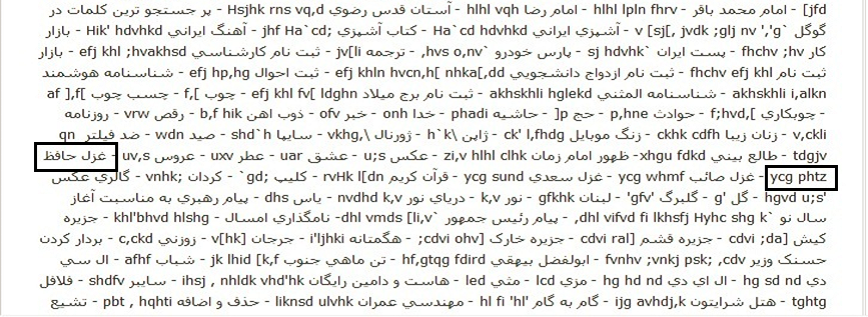
\includegraphics[scale=0.6]{Figures/spam1.png}
\caption{\label{fig:s1}
نمونه‌ای از یک صفحه هرز فارسی که از روش انباشتگی کلید‌واژه‌ها برای افزایش رتبه خود استفاده کرده است.
}
\end{figure}
\item
صفحاتی که دارای تعداد زیادی عکس و تبلیغ انواع محصولات مربوط به کالاهای مختلف و تقلبی هستند. در برخی از این صفحات، نسبت تعداد ارجاعات به صفحات تبلیغاتی مختلف در آن‌ها، به میزان متن مفید صفحه بسیار زیاد است. نکته‌ای که در مورد این صفحات باید در نظر گرفت این است که صفحات معتبر تبلیغاتی که مربوط به شرکت­های تبلیغاتی معتبر هستند و یا اطلاعات مفیدی هم‌چون مقایسه قیمت و کیفیت کالا، تلفن و آدرس شرکت‌ها و یا سازمان‌های خصوصی و دولتی را در اختیار کاربران قرار می‌دهند، جزء صفحات هرز محسوب نمی‌شوند.
\item
صفحاتی که شامل کلمات متنوعی هستند که به صورت خودکار و تصادفی توسط ماشین ایجاد شده‌اند. برخی از این کلمات دارای خطای املایی و نوشتاری هستند. برخی از آن‌‌ها نیز به همراه مدل نوشتاری انگلیسی صفحه کلید ظاهر می‌شوند. با استفاده از این روش، این صفحات می‌توانند در شرایطی که زبان صفحه کلید به اشتباه بر روی حالت انگلیسی است و کاربر کلمات موردنظر را به فارسی وارد می‌کند، رتبه خوبی را بدست آورند. برای مثال، همان‌طور که در شکل \ref{fig:s2} مشاهده می‌کنیم، مدل نوشتاری انگلیسی عبارت «غزل حافظ»  به صورت «\lr{ycg phtz}» نوشته می‌شود.
\begin{figure}
\centering
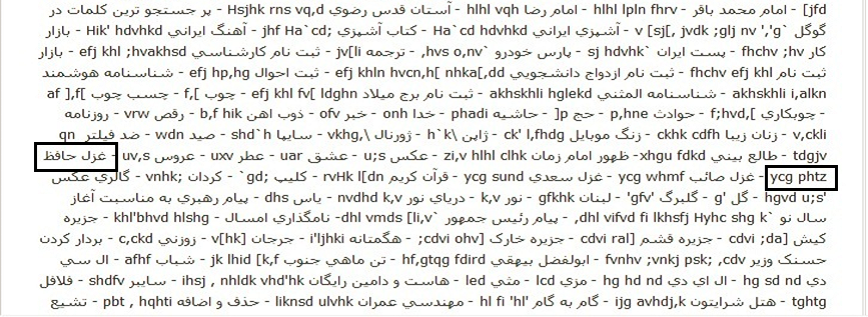
\includegraphics[scale=0.6]{Figures/spam2.png}
\caption{\label{fig:s2}
بخشی از یک صفحه هرز که دارای کلیدواژه‌های زیاد به همراه مدل نوشتاری انگلیسی آن‌ها می‌باشد.
}
\end{figure}
%\item
%صفحاتی که دارای جملاتی هستند که معنای خاصی نداشته و صرفا متشکل از تعدادی کلمه هستند که به طور تصادفی کنار هم  قرار گرفته­اند. این‌گونه صفحات می توانند به صورت دستی و یا خودکار ایجاد شوند.
\item
صفحاتی که دارای بخش‌های متنی نامرتبط با یکدیگر هستند. یک هرزنویس برای ایجاد چنین صفحه‌ هرزی معمولا بخش‌های مختلفی از متن وب‌گاه‌های معتبر را در صفحه خود رونوشت می‌کند. بنابراین با خواندن متن صفحه می‌توان مشاهده نمود که این صفحه دارای محتوای پیوسته و مفید نمی‌باشد و جملات متوالی از نظر مفهومی ارتباطی با یکدیگر ندارند. همچنین برخی از جملات در این صفحه نیمه‌کامل می‌باشند. نمونه‌ای از این صفحات در شکل \ref{fig:s3} ارائه شده است. 
%نکته‌ای که در مورد این نوع  از صفحات باید در نظر داشت، این است که صفحاتی که محتوای آن‌ها  شامل متن‌های ادبی، جملات بزرگان و اشعار معروف هستند از جمله صفحات معتبر و مفید شناخته می شوند.
\begin{figure}
\centering
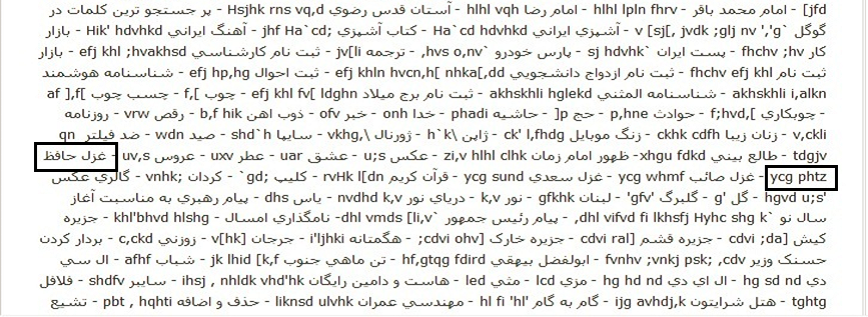
\includegraphics[scale=0.6]{Figures/spam3.png}
\caption{\label{fig:s3}
بخشی از یک صفحه هرز که دارای جمله‌های نیمه‌کاره و مطالب نامرتبط با یکدیگر می‌باشد.
}
\end{figure}

\item
صفحاتی که دارای تعداد زیادی پیوند غیرمفید هستند. این پیوندها معمولا به صفحات نامربوط، صفحات مسدود شده، صفحات هرز و یا صفحات درون همان وب‌گاه که دارای محتوای تکراری هستند، اشاره می‌کنند. در برخی مواقع نیز با تلیک بر روی یک پیوند، کاربر مجددا به همان صفحه هدایت می‌شود. برخی از این پیوندها نیز شبه‌پیوند هستند و در صورت تلیک کردن بر روی آن‌ها اتفاق خاصی نمی‌افتد.
%برای نمونه در سایت زیر مشاهده می کم که با کلیک کردن بر روی لینک «دانلود آهنگ های منصور» مجددا همان صفحه نمایش داده میشود و فقط برچسب آن تغییر یافته است و در اصل امکان دانلود آهنگ موردنظر وجود ندارد.
\item
صفحاتی که دارای محتوای مخفی، مانند بخش‌هایی از متن صفحه و یا پیوندهای پنهان هستند. با استفاده از روش‌هایی مانند استفاده از رنگ پیش‌زمینه صفحه و یا نوشتن متن با اندازه بسیار کوچک، این بخش‌ها از دید کاربر پنهان می‌­مانند، اما همچنان توسط موتورهای جست‌و‌جو \mls{نمایه‌سازی} شده و امتیاز آن‌ها در محاسبه رتبه صفحه در میان سایر نتایج پرس‌وجو در نظر گرفته می‌شود. برای پیدا کردن این بخش‌ها می‌توان از \lr{Ctrl+A} استفاده کرد. 
%برای مثال همان‌طور که در شکل \ref{fig:s6-2} مشاهده می‌نماییم در ابتدا به ظاهر در این بخش از صفحه، هیچ متنی وجود ندارد. پس از فشردن کلیدهای \lr{Ctrl+A}، متن‌های پنهان شده در صفحه مشخص می‌شوند.
لازم به ذکر است که وجود اطلاعات پنهان، مانند تاریخ به‌روزرسانی وب‌گاه، که مربوط به مشخصات و یا تنظیمات صفحه است، نشان‌گر یک صفحه هرز نمی‌باشد.

%\begin{figure}
%\begin{subfigure}{0.5\textwidth}
  %\centering
  %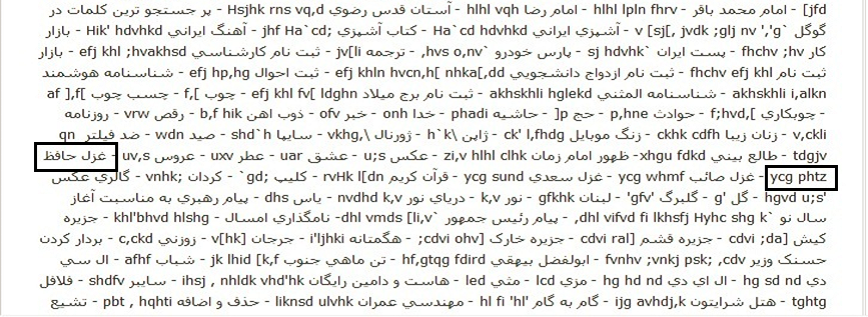
\includegraphics[width=0.8\linewidth]{Figures/spam2.png}
 % \caption{1a}
  %\label{fig:sfig1}
%\end{subfigure}%
%\begin{subfigure}{.5\textwidth}
 % \centering
  %\includegraphics[width=0.8\linewidth]{Figures/spam6-2.png}
  %\caption{1b}
  %\label{fig:sfig2}
%\end{subfigure}
%\caption{plots of....}
%\label{fig:fig}
%\end{figure}


%\includegraphics[scale=0.6]{Figures/spam6-2.png}
%\caption{\label{fig:s6-2}
%بخشی از یک صفحه هرز که دارای  محتوای پنهان می‌باشد.
\item
صفحاتی که \lr{URL} آن­ها شامل کلیدواژه‌های زیاد و علامت‌های نگارشی مختلف مانند نقطه و خط تیره است. با توجه به این‌که موتورهای جست‌و‌جو، آدرس صفحات را نیز نمایه‌سازی می‌کنند و از کلمات درون آن‌ها نیز برای رتبه‌دهی به صفحه استفاده می‌نمایند، در این نوع از صفحات با استفاده از کلیدواژه‌ها در آدرس صفحه، سعی می‌کنند رتبه خود را افزایش دهند.
برای مثال آدرس \lr{.html}خرید-شال-زنانه-طرح-قلب-و-طاووس\lr{http://www.mihanmobile.net/} که مربوط به یک وب‌گاه هرز است و دارای تعدادی کلمه کلیدی که با استفاده از خط تیره جدا شده‌اند، می‌باشد.
%pulsitemeter.com/bazar/bazar-kharid-laptop-iran.html
\item
صفحاتی که دارای نظرها و انجمن‌های گفتگوی رونوشت شده می‌باشند. این دسته از صفحات، به ظاهر دارای بخش‌ها و انجمن‌هایی هستند که در آن امکان تبادل نظر و ارسال پیام وجود دارد، اما در اصل چنین امکانی برای کاربران فراهم نشده است. همچنین برخی از این صفحات دارای کلیدهایی به نام «ادامه مطلب»، «خرید کالا»، «دانلود» و «ارسال نظر» هستند که در صورت تلیک کردن بر روی آن‌ها هیچ اتفاقی رخ نمی‌دهد. 
\item
صفحاتی که قبل از بارگذاری، کاربر را به صفحه‌ای با دامنه متفاوت هدایت می‌کنند. همچنین صفحاتی که با تلیک کردن بر روی پیوند آن‌ها، علاوه بر آن صفحه، یک یا چند صفحه تبلیغاتی نیز به طور خودکار باز می‌شود.  
برای نمونه، با وارد کردن آدرس «\lr{http://100cd.ir}» در نوار آدرس، مرورگر به طور خودکار به آدرس «\lr{http://shop.sarzamindownload.com}» هدایت می شود.
\end{itemize}

با توجه به این‌که در این پژوهش برچسب‌زنی را در سطح میزبان در نظر گرفته‌ایم، تعریف یک وب‌گاه هرز را به صورتی تقریبا متفاوت در نظر می‌گیریم. 
مطابق این تعریف، در صورتی که علاوه بر صفحه  اصلی یک وب‌گاه، حداقل پنج صفحه از میان ده صفحه‌ای که از آن وب‌گاه به صورت تصادفی انتخاب شده است هرز باشد، آن وب‌گاه به عنوان یک وب‌گاه هرز شناسایی می‌شود. همچنین با بررسی وب‌گاه‌ها، درمی‌یابیم که در صفحات یک وب‌گاه هرز معمولا از ترکیب تعدادی از روش‌های بالا  استفاده می‌شود.

\subsubsection{جمع‌آوری فهرستی از مجموعه وب‌گاه‌های فارسی}
با توجه به این‌که وجود وب‌گاه‌های هرز، نارضایتی کاربران زیادی را به همراه دارد، با جست‌و‌جو در میان وب‌گاه‌ها و وب‌نوشت‌های مختلف، می‌توان فهرستی از صفحاتی را که توسط کاربران وب به عنوان صفحات هرز گزارش شده‌اند، جمع‌آوری نمود. در این پژوهش علاوه بر استفاده از این روش، به صورت مستقیم نیز  فهرستی  از وب‌گاه‌های هرز و معتبر را از مراکز تحقیقاتی مختلف جمع‌آوری نمودیم. 

همچنین، برای تهیه فهرستی از وب‌گاه‌های معتبر، می‌توان از آدرس مربوط به وب‌گاه‌های دولتی،  شرکت‌ها و یا سازمان‌های معتبر استفاده کرد. در این پژوهش از وب‌گاه‌ \lr{http://www.i-link.ir} که شامل فهرستی از وب‌گاه‌های معتبر در موضوعات مختلف می‌باشد، استفاده نمودیم. در این وب‌گاه، آدرس بسیاری از صفحات معتبر و مفید فارسی، به صورت دسته‌بندی شده قرار دارد. برای مثال وب‌گاه‌های مربوط به دانشگاه‌ها، مراکز آموزشی، مراکز درمانی، بانک‌ها، مراکز تجاری، وب‌گاه‌های خبری و ورزشی، هر یک به صورت مجزا دسته‌بندی شده‌اند. برای جلوگیری از سوگیری وب‌گاه‌های معتبر به سمت یک موضوع خاص، وب‌گاه‌ها را از تمام موضوعات انتخاب کردیم.

با توجه به این‌که برای ساخت مجموعه داده‌ای موردنظر، روش برچسب‌زنی در سطح میزبان را انتخاب نموده‌ایم، پس از جمع‌آوری آدرس صفحات فارسی مختلف، فهرست وب‌گاه‌های یکتا را از آن‌ها استخراج نمودیم. 

\subsubsection{خزش اولیه وب‌گاه‌ها}
پس از فراهم کردن فهرستی از آدرس وب‌گاه‌های فارسی، می‌توان محتوای آن‌‌ها را  با استفاده از یک خزشگر مناسب ذخیره نمود و در مراحل بعد از محتوای صفحات  به صورت برون‌خط استفاده کرد. در این مرحله، پیدا کردن یک خزشگر مناسب برای  وظیفه موردنظر از اهمیت ویژه‌ای برخوردار است. بدین منظور پس از بررسی قابلیت‌ها و ضعف‌های تعدادی از خزشگرهای موجود، در نهایت از دو خزشگر برای ساخت مجموعه داده‌ای موردنظر استفاده نمودیم. 
در ابتدا با توجه به قابلیت‌ها و واسط کاربری مناسبی که خزشگر \lr{Offline Explorer}‌\LTRfootnote{http://www.metaproducts.com/OE.html} دارد، از آن برای خزش فهرست اولیه وب‌گاه‌ها استفاده کردیم. این خزشگر این امکان را فراهم می‌کند که با یک بار اجرا و تنظیم سطح خزش وب‌گاه‌ها، تمام صفحات یک وب‌گاه را به طور کامل خزش کرده و به صورت برون‌خط از آن استفاده نماییم. در واقع این خزشگر  یک مرورگر را شبیه‌سازی می‌کند که در آن می‌توان با تلیک کردن بر روی پیوندهای مختلف درون یک صفحه، به صفحات دیگر آن وب‌گاه و همچنین سایر صفحات مربوط به پیوندهای درون صفحه رفت. یکی از مزیت‌‌هایی که این خزشگر دارد، واسط کاربری مناسب و امکان انجام تنظیماتی مانند انتخاب و یا حذف بخش‌های مختلف صفحه از جمله عکس‌ها، فیلم و فایل‌های با فرمت خاص، در هنگام خزش می‌باشد.

پس از خزش وب‌گاه‌ها، به صورت برون‌خط و با استفاده از شبیه‌ساز مرورگر در \lr{Offline Explorer}، یک بررسی اجمالی بر روی وب‌گاه‌های خزش شده انجام داده و وب‌گاه‌هایی را که شرایط موردنظر را ندارند، از فهرست حذف کردیم.
برای مثال، یکی از مشکلاتی که در بررسی وب‌گاه‌ها به آن برخوردیم، سرعت از بین رفتن وب‌گاه‌های هرز می‌باشد. موتورهای جست‌و‌جو علاوه بر استفاده از انواع روش‌های شناسایی هرز وب و مقابله با صفحات هرز به صورت برخط، فهرست سیاهی از صفحات و وب‌گاه‌های هرز را نیز تهیه می‌کنند. با داشتن این فهرست در هنگام بازیابی نتایج، صفحات هرز درون این فهرست، توسط موتورهای جست‌و‌جو نمایه‌سازی‌‌‌ نمی‌شوند. هرزنویسان برای فرار از این مشکل، معمولا پس از مدت زمان مشخصی، آدرس وب‌گاه‌های خود را تغییر می‌دهند که این امر باعث می‌شود بسیاری از نام‌های میزبان مربوط به وب‌گاه‌های هرز بدون استفاده باقی بماند. در نتیجه این نوع از وب‌گاه‌ها را که تعداد قابل توجهی داشتند، از فهرست وب‌گاه‌های موردنظر حذف نمودیم. 


\subsubsection{جمع‌آوری وب‌گاه‌های هرز}
پس از بررسی اجمالی وب‌گاه‌های خزش شده و پالایش آن‌‌ها، تعداد زیادی از وب‌گاه‌های هرز از میان فهرست وب‌گاه‌ها حذف شدند و تنها تعداد محدودی از آن‌ها باقی ماندند. بنابراین برای تکمیل مجموعه داده‌ای، همچنان به وب‌گاه‌های هرز بیشتری نیاز داشتیم.
از طرف دیگر، با توجه به این‌که درصد وب‌گاه‌های هرز به نسبت وب‌گاه‌های معتبر بسیار کمتر می‌باشد، مشکل اصلی در ایجاد پیکره‌ای از وب‌گاه‌های هرز و معتبر، پیدا کردن وب‌گاه‌های هرز می‌باشد. بدین منظور از روش‌های دیگری برای جمع‌آوری این نوع از وب‌گاه‌ها استفاده کردیم که در ادامه به شرح آن‌ها می‌پردازیم. 

در این مرحله، با در نظر گرفتن این امر که در میان پیوندهای درون یک صفحه هرز، معمولا تعدادی ارجاع  به سایر صفحات هرز وجود دارد، با دنبال کردن مسیر پیوندهای خروجی از صفحات هرز، به دنبال جمع‌آوری صفحات هرز جدید پرداختیم. بدین منظور ابتدا فهرست آدرس‌های مجموعه وب‌گاه‌های هرز باقی‌مانده از مرحله قبل را به عنوان بذر اولیه به خزشگر \lr{Offline Explorer} داده و صفحات را تا سه سطح خزش کردیم. با توجه به این‌که تمرکز ما در این مرحله بیشتر بر روی پیدا کردن وب‌گاه‌های هرز می‌باشد، بعد از خزش سطح اول، خزشگر را متوقف کرده و صفحات خزش شده جدید را بررسی نمودیم. از میان این صفحات، مجددا فهرست مربوط به وب‌گاه‌های یکتا و جدید را استخراج کرده و پس از بررسی اجمالی آن‌ها و حذف وب‌گاه‌های مسدود شده، وب‌گاه‌های هرز باقی‌مانده را به عنوان بذر به خزشگر دادیم. سپس فرآیند مرحله اول را مجددا تکرار نمودیم. 

برای جلوگیری از سوگیری وب‌گاه‌های هرز به سمت یک مجموعه بذر مشخص، با استفاده از مجموعه کلیدواژه‌های رایج در پرس‌وجوها، به صورت تصادفی پرس‌وجوهای جدیدی ایجاد کرده و به موتورهای جست‌و‌جوی مختلف مانند گوگل و بینگ دادیم. نمونه‌هایی از این کلمات،  «دانلود»، «عکس»، «بازی»، «آهنگ» و «فیلم» می‌باشد که طبق آمار گزارش شده توسط گوگل \LTRfootnote{http://www.google.com/trends/}، به ترتیب بالاترین میزان استفاده را  در پرس‌وجو‌های دو سال اخیر داشته‌اند. با توجه به این‌که محدود کردن پرس‌وجو‌ها به این کلمات، نتایج را به سمت وب‌گاه‌های مشخص و محدودی متمایل می‌کند، از حدود صد کلمه رایج در پرس‌وجوها استفاده نمودیم و آن‌ها را  با توجه به میزان ارتباطشان با یکدیگر به ده گروه تقسیم کردیم. سپس در هر گروه تعداد دو یا سه کلمه از آن را به صورت تصادفی کنار هم گذاشته و بدین ترتیب تعداد زیادی پرس‌وجو ایجاد نمودیم. 
پس از آن به ازای هر پرس‌وجو، ده نتیجه اول را بررسی کردیم. با توجه به این‌که صفحات هرز معمولا دارای تعداد زیادی کلیدواژه هستند، در میان نتایج بازیابی شده توسط موتور جست‌وجوی  بینگ، به ازای هر پرس‌و‌جو به طور متوسط حدود دو الی سه صفحه هرز وجود داشت که البته بسیاری از آن‌ها مربوط به یک وب‌گاه مشترک بودند. 

\subsubsection{برچسب‌زنی وب‌گاه‌ها}
پس از مشخص کردن فهرست نهایی آدرس وب‌گاه‌های خزش شده، برچسب وب‌گاه‌ها را مشخص نمودیم. برای این کار، با داشتن محتوای وب‌گاه‌ها به صورت برون‌خط، برای ساده‌سازی و افزایش سرعت برچسب‌زنی وب‌گاه‌ها، برنامه‌ای نوشتیم که دارای واسط گرافیکی با گزینه‌هایی برای مشخص کردن زبان صفحه، برچسب آن، نوع هرز بودن آن و اعلام تغییر خودکار آدرس صفحه به صفحه‌ای دیگر می‌باشد. با استفاده از این برنامه،‌ می‌توان محتوای مجموعه‌ای از وب‌گاه‌ها را بررسی کرده و برچسب آن‌ها را مشخص نماییم. 

%\subsubsection{استفاده از ضریب کاپا برای افزایش دقت برچسب‌زنی}
\subsubsection{خزش نهایی و ذخیره مجموعه وب‌گاه‌ها}
پس از برچسب‌زنی نهایی وب‌گاه‌ها، برای خزش نهایی آن‌ها از  \lr{HtmlUnit}\LTRfootnote{http://htmlunit.sourceforge.net/} که به زبان جاوا می‌باشد استفاده نمودیم. دلیل استفاده از این خزشگر، امکان خزش کردن بخش‌های پویای صفحه مانند کدهای جاوا اسکریپت و محتوای درون \lr{i-frame}ها می‌باشد. 
% این بخش‌ها در خزشگر \lr{Offline Explorer} به صورت مجزا از هم خزش شده و ترتیب آن‌ها رعایت نمی‌شود. 
همچنین با استفاده از این خزشگر می‌توان هم‌زمان فرآیند هنجارسازی متن صفحه و جداسازی بخش‌های مختلف آن را انجام داد. 

پس از انجام مراحل بالا، در نهایت 300 وب‌گاه هرز فارسی و 1050 وب‌گاه معتبر فارسی جمع‌آوری، خزش و نمایه‌سازی شدند. اطلاعات مربوط به خصوصیات آماری این مجموعه داده‌ای در ادامه در بخش \ref{section:experiments-datasets}  ارائه شده است. 

\subsection{معرفی و تحلیل ویژگی‌های محتوایی بر روی وب‌گاه‌های فارسی}
\label{section:methodology-structuralcontentbased}
در این بخش، ابتدا به توضیح مختصر ویژگی‌های محتوایی که توسط \lr{Ntoulas} و همکاران \cite{Ntoulas:2006} معرفی شده است می‌پردازیم. سپس با معرفی ویژگی‌های محتوایی ارائه شده در \cite{Fetterly:2004, Prieto:2013, Urvoy:2008tracking} رفتار وب‌گاه‌های هرز فارسی را بر اساس مقادیر مختلف هر یک از این ویژگی‌ها تحلیل می‌کنیم. در نهایت برای بهبود کارایی رده‌بند نهایی، تعدادی ویژگی جدید معرفی می‌نماییم.

\subsubsection{ویژگی‌های گروه ۱: ویژگی‌های پایه}
%\label{section:methodology-featureset1}
پس از ساخت مجموعه داده‌ای برچسب خورده شامل وب‌گاه‌های فارسی، در مرحله اول، ویژگی‌های محتوایی معرفی شده در مقاله \cite{Ntoulas:2006} را به عنوان ویژگی‌های \mls{پایه}، از وب‌گاه‌های فارسی استخراج کرده و میزان تاثیر آن‌‌ها را در شناسایی وب‌گاه‌های هرز فارسی بررسی نمودیم. این ویژگی‌ها عبارتند از:
\begin{itemize}
\item
تعداد کلمات هر صفحه: یکی از روش‌های رایج در میان هرزنویسان، روش انباشتگی کلید‌واژه‌ها است. در این روش با استفاده از انواع کلیدواژه‌ها و تکرار آن‌ها درون صفحات خود سعی می‌کنند رتبه صفحه خود را به ازای پرس‌وجوهای بیشتری بالا ببرند. بنابراین تعداد کلمات در این نوع از صفحات هرز به طور متوسط از صفحات معتبر بیشتر می‌باشد.
\item
تعداد کلمات عنوان هر صفحه: با توجه به این‌که برخی از موتورهای جست‌و‌جو به کلمات درون عنوان صفحات وزن بیشتری اختصاص می‌دهند، در بسیاری از صفحات هرز از روش انباشتگی کلید‌واژه‌ها در عنوان صفحه استفاده می‌شود.
\item
متوسط طول کلمات موجود در صفحه: یکی از روش‌های دیگری که هرزنویسان برای بالا بردن رتبه صفحه خود به‌کار می‌برند، استفاده از کلمات ترکیبی است که از اتصال دو تا سه کلمه به یکدیگر ایجاد می‌شوند. با استفاده از این روش هرزنویسان می‌توانند رتبه صفحه خود را به ازای پرس‌وجوهایی که کاربران فراموش می‌کنند بین کلمات آن از فاصله استفاده کنند بالا ببرند. بنابراین انتظار می‌رود که در این نوع از صفحات هرز، متوسط طول کلمات بیشتر از صفحات معتبر باشد.
\item
درصد متن پیوند درون هر صفحه: هرزنویسان برای بالا بردن رتبه صفحات خود تعداد زیادی صفحه ایجاد می‌کنند که به صفحات موردنظر ارجاع می‌دهند. این صفحات معمولا محتوای زیادی ندارند و دارای تعداد زیادی پیوند هستند که هر کدام به صفحاتی با موضوعات مختلف اشاره می‌کنند. بنابراین در این‌گونه صفحات هرز، درصد بیشتری از صفحه با استفاده از متن پیوند پر شده است که معمولا دارای کلیدواژه‌ها با موضوعات مختلف می‌باشند.
\item
درصد محتوای قابل مشاهده در هر صفحه: برخی از موتورهای جست‌و‌جو برای پیدا کردن نتایج مرتبط با پرس‌وجوهای کاربران، علاوه بر متن اصلی صفحات،  بخش‌هایی از محتوای صفحات را نیز که درون ابربرچسب‌های \lr{HTML} می‌باشد، نمایه‌سازی می‌کنند. ابربرچسب‌های درون بخش \lr{header} صفحه و برچسب  \lr{ALT} مربوط به تصاویر درون صفحه، که دارای توضیحاتی پیرامون تصاویر مربوطه است، نمونه‌هایی از این بخش‌ها می‌باشند. با توجه به این رفتار موتورهای جست‌و‌جو، هرزنویسان برای بالا بردن رتبه صفحات هرز خود، از روش انباشتگی کلید‌واژه‌ها در این بخش‌ها استفاده می‌کنند. 
%استفاده از این ویژگی می‌توان صفحات هرزی را که در آن‌ها از روش انباشتگی کلید‌واژه‌ها در بخش‌هایی از صفحه، که از دید کاربران پنهان می‌ماند، استفاده شده استشناسایی کرد. در این‌گونه صفحات با استفاده از تکرار کلمات درون بخش‌ها بخش‌هایی از متن که دارای تعداد زیادی کلیدواژه‌های مرتبط و نامرتبط با تکرار زیاد هستند، با استفاده از روش‌های پنهان‌سازی محتوا از دید کاربر پنهان می‌شود. به عنوان مثال اما با توجه به این‌که موتورهای جست‌و‌جو این بخش‌ از محتوا را نیز نمایه‌سازی می‌کنند، این روش در بالا بردن رتبه صفحات موثر می‌باشد.
\item
درصد فشرده‌سازی: با توجه به این‌که برخی از موتورهای جست‌و‌جو به صفحاتی که تعداد تکرار کلمات پرس‌وجو در آن‌ها بیشتر باشد وزن بیشتری می‌دهند، هرزنویسان معمولا کلیدواژه‌ها را به تعداد زیاد درون صفحات خود استفاده می‌کنند. با استفاده از الگوریتم‌های فشرده‌سازی مانند \lr{GZIP} \cite{Gzip} می‌توان درصد تکراری بودن محتوای صفحات را محاسبه کرد. برای محاسبه این ویژگی ابتدا هر صفحه را با استفاده از الگوریتم \lr{GZIP} فشرده کردیم. سپس اندازه صفحه را بر اندازه صفحه پس از فشرده‌سازی تقسیم نمودیم. هر چقدر مقدار این تقسیم بزرگتر باشد، بدین معنا می‌باشد که صفحه موردنظر، قابلیت فشرده‌سازی بیشتری دارد؛ به عبارت دیگر، محتوای تکراری در آن صفحه بیشتر بوده و در نتیجه احتمال هرز بودن آن صفحه نیز بیشتر می‌باشد.
\item
 %برخی از صفحات هرز برای بالا بردن رتبه خود از تعداد زیادی کلمات پرکاربرد استفاده می‌کنند. با استفاده از این ویژگی می‌توان این دسته از صفحات را شناسایی کرد.%
درصدی از صفحه که شامل کلمات مشهور می‌باشد: برای محاسبه این ویژگی، کلمات پرتکرار موجود در مجموعه وب‌گاه‌ها استخراج شده و $n$ کلمه اول به عنوان مجموعه کلمات مشهور در نظر گرفته می‌شود. سپس به ازای هر صفحه، تعداد کلمات مشهور درون صفحه را، بر تعداد کل کلمات موجود در آن تقسیم می‌نماییم. انتظار می‌رود که با استفاده از این ویژگی بتوان وب‌گاه‌های هرزی را که به صورت تصادفی تعدادی از کلیدواژه‌ها را درون صفحات خود تکرار کرده‌اند، شناسایی کرد. در این‌گونه از وب‌گاه‌ها، معمولا درصد کلمات مشهور مانند ایست‌واژ‌ه‌ها، کمتر از درصد این کلمات در وب‌گاه‌های معتبر است.
%این ویژگی را به ازای مقادیر مختلف ۱۰۰، ۲۰۰، ۳۰۰، ۵۰۰ و ۱۰۰۰ برای $n$ محاسبه کردیم. پس از محاسبه و بررسی این ویژگی بر روی وب‌گاه‌های فارسی متوجه شدیم که این ویژگی برخلاف آن‌چه که در \cite{Ntoulas:2006} آمده در مورد وب‌گاه‌های فارسی تاثیر چندانی در شناسایی وب‌گاه‌های هرز ندارد. دلیل این امر این است که در میان $n$ کلمه مشهور موجود در پیکره فارسی، درصدی از آن‌‌ها ایست‌واژه‌ها بوده و درصد دیگری کلماتی هستند که به دلیل تکرار زیاد در وب‌گاه‌های هرز جزء $n$ کلمه مشهور انتخاب شده‌اند. همچنین درصد دیگری از کلمات کلماتی هستند که در بین وب‌گاه‌های معتبر رایج هستند و درصد دیگر کلماتی که بین هر دو دسته وب‌گاه به طور تقریبا یکنواخت توزیع شده‌اند. بنابراین اجتماع این کلمات با یکدیگر نمی‌تواند معیار خوبی برای رده‌بندی این دو نوع وب‌گاه باشد.
\item
درصدی از کلمات مشهور که در صفحه استفاده شده است: این ویژگی مکمل ویژگی قبلی است و نشان می‌دهد که چند درصد از کلمات مشهوری که در متن استفاده شده‌اند از یکدیگر متمایز هستند. برای محاسبه این ویژگی، تعداد کلماتی از مجموعه کلمات مشهور، که در متن آمده است را بر $n$، که همان تعداد کل کلمات مشهور می‌باشد، تقسیم می‌نماییم. با استفاده از این ویژگی می‌توان وب‌گاه‌های هرزی را شناسایی کرد که برای فریب ویژگی قبل، یک یا چند کلمه مشهور را به تعداد زیاد درون صفحات خود تکرار می‌کنند. تعداد کلمات مشهور یکتا در این‌گونه از وب‌گاه‌های هرز، نسبت به  وب‌گاه‌های معتبر کمتر می‌باشد. 

%با استفاده از این ویژگی می‌توان خطای ناشی از اختلاف طول اسناد را کاهش داد. برای مثال در صورتی که یک صفحه فقط دارای دو کلمه باشد که یکی از آن‌‌ها جزء کلمات مشهور باشد، مقداری که برای ویژگی قبلی برای این صفحه محاسبه می‌شود ۵۰ درصد است. در صورتی که، با استفاده از این ویژگی می‌توان فهمید که تنها یک کلمه از کلمات مشهور در این صفحه استفاده شده است. بنابراین این صفحه
%این ویژگی را نیز به ازای مقادیر مختلف ۱۰۰، ۲۰۰، ۳۰۰، ۵۰۰ و ۱۰۰۰ برای $n$ محاسبه کردیم. این ویژگی نیز به همان دلیلی که برای ویژگی قبل توضیح دادیم در تشخیص وب‌گاه‌‌های هرز فارسی کارایی قابل توجهی ندارد. %برای مثال در صورتی که یک صفحه فقط دارای دو کلمه باشد که یکی از آن‌‌ها جزء کلمات مشهور باشد مقداری که برای ویژگی قبلی برای این صفحه محاسبه می‌شود ۵۰ درصد است در صورتی که با استفاده از این ویژگی می‌توان فهمید که تنها یک کلمه از کلمات مشهور در این صفحه استفاده شده است.%
\item
\mls{احتمال شباهت $n$-گرام‌‌های مستقل}: این ویژگی میزان تکراری بودن محتوای صفحات را در سطح $n$-گرام محاسبه می‌کند. با استفاده از این ویژگی می‌توان دو نوع از وب‌گاه‌های هرز را شناسایی کرد. نوع اول وب‌گاه‌هایی هستند که یک بخش از محتوای آن‌ها چندین بار درون صفحه تکرار شده است. دسته دوم وب‌گاه‌هایی هستند که با کپی کردن بخش‌های مختلف از صفحات مختلف دارای محتوای نامرتبط با یکدیگر می‌باشند. بنابراین، در صورتی که برای مقادیر این ویژگی دو حد آستانه حداقل و حداکثر تعریف نماییم، احتمال هرز بودن صفحات برای صفحات خارج از این بازه، بیشتر از صفحات داخل این بازه خواهد بود. این ویژگی به صورت زیر محاسبه می‌شود:
\begin{equation}
 	independent\text{-}likelihoods = -\frac{1}{k} \sum_{i=0}^{(k-1)} \log P(w_{i+1}, ..., w_{i+n})
	\label{Eq:indlh}
\end{equation}
که در آن $P(w_{i+1}, ..., w_{i+n})$ احتمال $(i+1)$امین   $n$-گرام است که با تقسیم تعداد رخداد این  $n$-گرام به تعداد کل  $n$-گرام‌ها محاسبه می‌شود. 
%این ویژگی را به ازای $n=1, 2, 3, 4, 5$ محاسبه کردیم.
\item
\mls{احتمال شباهت $n$-گرام‌های شرطی}: این ویژگی مانند ویژگی قبل است، با این تفاوت که برای محاسبه ویژگی قبل، $n$-گرام‌ها به طور مستقل از هم در نظر گرفته می‌شوند. در صورتی که برای محاسبه این ویژگی، احتمال هر $n$-گرام به شرط وجود $(n-1)$ کلمه اول آن محاسبه می‌شود. نحوه محاسبه این ویژگی به صورت زیر است:
%این ویژگی را برای مقادیر $n=2, 3, 4, 5$ محاسبه کردیم.
\begin{equation}
 	conditional\text{-}likelihoods = -\frac{1}{k} \sum_{i=0}^{(k-1)} \log P(w_n|w_{i+1}, ..., w_{i+n-1})
	\label{Eq:condlh}
\end{equation}
به طوری‌که؛
\begin{equation}
 	P(w_n|w_{i+1}, ..., w_{i+n-1}) = \frac{P(w_{i+1}, ..., w_{i+n})}{P(w_{i+1}, ..., w_{i+n-1})}
	\label{Eq:condp}
\end{equation}
\end{itemize}

\subsubsection{ویژگی‌های گروه ۲: ویژگی‌های مکمل}
%\label{section:methodology-featureset2}
در مرحله بعد، برای شناسایی انواع بیشتری از وب‌گاه‌های هرز فارسی، تعدادی ویژگی محتوایی دیگر \cite{Fetterly:2004, Prieto:2013, Urvoy:2008tracking} را از این صفحات استخراج کرده و میزان کارایی و تاثیر آن‌ها را در شناسایی وب‌گاه‌های هرز بررسی نمودیم. در ادامه هر یک از این ویژگی‌ها را به طور مختصر توضیح می‌دهیم.
\begin{itemize}
\item
تعداد عکس‌ها: با بررسی تعداد عکس‌های درون وب‌گاه‌های فارسی به نظر می‌رسد که هر چقدر تعداد عکس‌ها، درون یک صفحه بیشتر باشد، احتمال هرز بودن آن صفحه بیشتر است. این امر می‌تواند به این دلیل باشد که وب‌گاه‌های هرز معمولا با اهداف تبلیغاتی و تجاری ایجاد می‌شوند. استفاده از تصاویر تبلیغاتی مختلف در این‌گونه از صفحات می‌تواند در جذب مشتری تاثیر بسزایی داشته باشد. رفتار وب‌گاه‌های فارسی در برابر این ویژگی، برخلاف رفتاری است که توسط \lr{Prieto} و همکاران \cite{Prieto:2013} برای وب‌گاه‌های انگلیسی بیان شده است. نظر آن‌ها این است که با توجه به این‌که وب‌گاه‌های هرز اکثرا به صورت خودکار ایجاد شده و با مطالب تصادفی پر می‌شوند،  تعداد تصاویر موجود در آن‌ها کم می‌باشد.
\item
طول \lr{URL}: هر \lr{URL} دارای یک نام میزبان و نام دامنه است. برخلاف نام دامنه که محدود به تعداد مشخصی دامنه شناخته شده است، هر اسمی می‌تواند به عنوان نام میزبان انتخاب شود. برای انتخاب نام میزبان معمولا از اسامی مرتبط با موضوع صفحه، از عنوان صفحه و یا از مدل اختصاری آن استفاده می‌کنند. با توجه به این‌که برخی از موتورهای جست‌و‌جو، \lr{URL} وب‌گاه‌‌ها را نیز نمایه‌سازی می‌کنند، بسیاری از هرزنویسان، برای افزایش امتیاز صفحات هرز خود، از کلیدواژه‌های زیادی درون \lr{URL} صفحات خود استفاده می‌کنند. این کلمات معمولا با استفاده از علامت‌های نگارشی مختلف، مانند خط فاصله از یکدیگر جدا شده‌اند. با در نظر گرفتن این مهم، انتظار می‌رود به طور متوسط طول \lr{URL} وب‌گاه‌های هرز فارسی نسبت به وب‌گاه‌های معتبر بیشتر باشد.
\item
تعداد کلمات درون ابربرچسب کلیدواژه‌ها و توضیحات صفحه: در هر صفحه \lr{HTML} سه بخش عنوان، ابربرچسب کلیدواژه‌ها و ابربرچسب توضیحات وجود دارد که یک موتور جست‌و‌جو برای اطلاع از این‌که یک صفحه پیرامون چه موضوع یا موضوعاتی است، از محتوای این بخش‌ها استفاده می‌کند. در نتیجه این بخش از صفحات مکان خوبی برای هرزنویسان است که با استفاده از روش انباشتگی کلید‌واژه‌ها در آن‌ها، رتبه صفحه هرز خود را افزایش دهند. بررسی وب‌گاه‌های فارسی نشان می‌دهد که متوسط تعداد کلمات موجود در ابربرچسب کلیدواژه‌ها و توضیحات، برای وب‌گاه‌‌های هرز بیشتر از وب‌گاه‌های معتبر است.
\item
تعداد کلمات درون متن پیوند: در میان صفحات وب، صفحاتی هستند که دارای پیوندهای زیاد به صفحات مختلف به همراه توضیحاتی پیرامون آن صفحات هستند. با توجه به این‌که موتورهای جست‌و‌جو برای محاسبه امتیاز صفحات وب از کلمات درون متن پیوند مربوط به پیوندهای آن‌ها، که در سایر صفحات وجود دارد نیز استفاده می‌کنند، هرزنویسان برای افزایش رتبه صفحات درون وب‌گاه خود، صفحاتی را ایجاد می‌نمایند که دارای تعداد زیادی ارجاع به صفحات موردنظر، به همراه متن پیوند مربوط به آن‌ها می‌باشند. محاسبه این ویژگی برای وب‌گاه‌های فارسی نشان می‌دهد که این امر در میان وب‌گاه‌های فارسی، امری رایج می‌باشد.
\item
 \mls{شباهت کسینوسی} \cite{wong1987modeling} بین بخش‌های مختلف صفحه: هر صفحه وب را می‌توان به سه بخش اصلی عنوان، بدنه و متن پیوند تقسیم کرد. شباهت کسینوسی معیاری است که میزان شباهت دو متن را بر اساس روش‌های وزن‌دهی مختلف محاسبه می‌نماید. در نتیجه با استفاده از این معیار می‌توان میزان شباهت بین محتوای این سه بخش اصلی را محاسبه کرد. در این پژوهش، برای محاسبه این ویژگی از دو روش وزن‌دهی \mls{دودویی} و \lr{TF-IDF} استفاده کرده و شباهت کسینوسی بین هر زوج بخش اصلی را محاسبه نمودیم. بررسی رفتار وب‌گاه‌های فارسی نسبت به مقادیر مختلف این ویژگی نشان می‌دهد که احتمال هرز بودن وب‌گاه‌ها برای مقادیر کمتر از یک آستانه حداقلی و بیشتر از یک آستانه حداکثری افزایش می‌یابد. دلیل افزایش احتمال هرز بودن صفحات به ازای کاهش بیش از حد مقدار این ویژگی‌ها را می‌توان وجود صفحات هرزی دانست که با رونوشت بخش‌های مختلف از محتویات صفحات مختلف سعی دارند امتیاز صفحه خود را افزایش دهند. همچنین صفحاتی که مقدار این ویژگی برای آن‌ها از یک آستانه مشخص بیشتر است، صفحات هرزی هستند که برای افزایش رتبه صفحه خود از روش انباشتگی کلید‌واژه‌ها استفاده کرده‌اند.
\item
تعداد ایست‌واژه‌ها درون هر صفحه: یکی از روش‌‌های نمایه‌سازی رایج در موتورهای جست‌و‌جو، حذف ایست‌واژه‌ها قبل از نمایه‌سازی صفحات می‌باشد. بنابراین هرزنویسان با حذف ایست‌واژه‌ها از وب‌گاه‌های خود و با استفاده از قرار دادن کلیدواژه‌های تصادفی در آن‌ها، امتیاز وب‌گاه خود را به ازای پرس‌وجوهای زیادی بالا می‌برند. بنابراین انتظار می‌رود با استفاده از این ویژگی بتوان وب‌گاه‌های هرزی را که با این روش تولید می‌شوند شناسایی کرد. اما همان‌طور که در مقاله \cite{Prieto:2013} نشان داده می‌شود که این ویژگی تاثیر چندانی در شناسایی این دسته از وب‌گاه‌های هرز ندارد، با بررسی وب‌گاه‌های هرز فارسی نیز به چنین نتیجه‌ای رسیدیم. برای رفع این مشکل، در ادامه در بخش ویژگی‌های جدید، مدل بهبود یافته‌ای از این ویژگی را با عنوان «درصدی از صفحه که از ایست‌واژه‌ها تشکیل شده‌است»، معرفی می‌نماییم. 
\item
تعداد پیوندهای خروجی: برخی از صفحات هرز، فقط با هدف افزایش \lr{PageRank} سایر صفحات هرز ایجاد می‌شوند. این صفحات معمولا بخشی از یک دهکده پیوندی هستند که با دادن ارجاعات زیاد به سایر صفحات هرز، که معمولا مربوط به یک وب‌گاه مشترک می‌باشند، سعی بر افزایش رتبه آن صفحات و درنتیجه افزایش رتبه صفحه خود را دارند. پس از تحلیل این ویژگی بر روی وب‌گاه‌های فارسی به این نتیجه رسیدیم که احتمال هرز بودن یک وب‌گاه با افزایش تعداد پیوند‌های خروجی از آن وب‌گاه افزایش می‌یابد. 
\end{itemize}

\subsubsection{ویژگی‌های گروه ۳: ویژگی‌های جدید}
%\label{section:methodology-featureset3}
در این مرحله برای بهبود رده‌بندی وب‌گاه‌های فارسی تعدادی ویژگی جدید معرفی می‌نماییم. ابتدا این ویژگی‌ها را از مجموعه داده‌ای فارسی استخراج کرده و پس از رسم نمودار توزیع وب‌گاه‌ها برای هر یک از ویژگی‌ها به طور مجزا و تحلیل هر یک از آن‌‌ها، میزان تاثیر آن‌‌ها را در نتیجه نهایی رده‌بندی محاسبه کردیم. این ویژگی‌ها به شرح زیر می‌باشند:
\begin{itemize}
\item
مجموع اندازه عکس‌های درون هر صفحه: بررسی تعداد زیادی از وب‌گاه‌های فارسی نشان می‌دهد که به طور متوسط، تعداد تصاویر و مجموع اندازه آن‌ها در وب‌گاه‌های هرز، بیشتر از وب‌گاه‌های معتبر می‌باشد. در این‌گونه از وب‌گاه‌های هرز، درصد محتوای متنی درون صفحه، کمتر از سایر وب‌گاه‌ها می‌باشد. هدف از این امر، تبلیغ محصولات و جذب مشتری و رسیدن به سایر اهداف تجاری می‌باشد. بزرگ بودن تصاویر، علاوه بر این‌که در جذب مشتری تاثیر قابل توجهی دارد، احتمال تلیک کردن بر روی آن تصاویر و رفتن به صفحات تبلیغاتی مربوط به آن را افزایش می‌دهد. بنابراین علاوه بر تعداد عکس‌های درون هر صفحه، مجموع اندازه عکس‌هایی که در هر صفحه نمایش داده می‌شود را به عنوان یک ویژگی جدید به سایر ویژگی‌ها اضافه کردیم. نمودار \ref{fig:plot1} توزیع وب‌گاه‌های فارسی و همچنین احتمال هرز بودن این وب‌گاه‌ها را به ازای مقادیر مختلف این ویژگی نشان می‌دهد. با توجه به این نمودار، با افزایش مجموع اندازه عکس‌های درون هر وب‌گاه، احتمال هرز بودن آن وب‌گاه نیز افزایش می‌یابد.
\begin{figure}
\centering
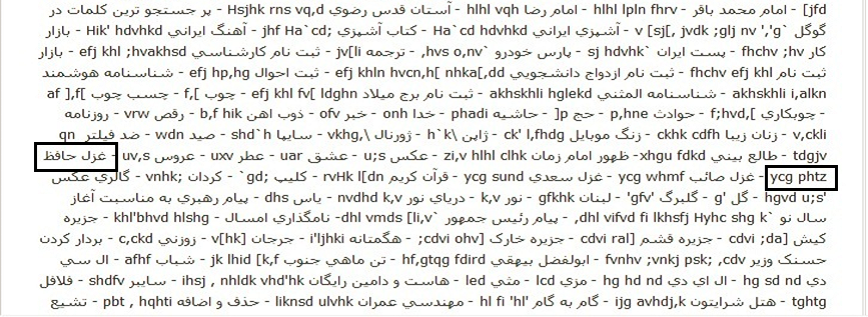
\includegraphics[scale=0.7]{Figures/plot1.png}
\caption{\label{fig:plot1}
رفتار وب‌گاه‌های فارسی به ازای مقادیر مختلف ویژگی «مجموع اندازه عکس‌های درون هر صفحه»
}
\end{figure}
\item
تعداد منابع چند‌رسانه‌ای درون هر صفحه: خصوصیت دیگری که در زمان بررسی وب‌گاه‌های هرز فارسی مشاهده می‌نماییم، استفاده هرزنویسان از منابع چند رسانه‌ای برای جذب کاربران به سمت صفحات خود و یا سایر وب‌گاه‌های هرز می‌باشد. برای مثال یک کاربر با ورود به یک صفحه هرز که محتوای مفیدی ندارد اما به صورت خودکار موسیقی زیبایی را پخش می‌نماید، برای گوش دادن به موسیقی مدت زمان بیشتر را در آن صفحه می‌ماند. با توجه به نمودار \ref{fig:plot2} مشاهده می‌نماییم که با افزایش مقدار این ویژگی، احتمال هرز بودن وب‌گاه‌های فارسی در کل یک روند صعودی دارد. همان‌طور که در نمودار مشخص است، به ازای مقدار ۷۱۲ برای تعداد منابع چندرسانه‌ای،  میزان احتمال هرز بودن وب‌گاه‌ها صفر می‌باشد. دلیل این امر کوچک بودن مجموعه ‌داده‌ای فارسی در مقایسه با تعداد کل صفحات وب می‌باشد که باعث می‌شود پراکندگی وب‌گاه‌ها بر روی مقادیر مختلف یک ویژگی یکنواخت نباشد. در نتیجه با توجه به این‌که در این بازه هیچ وب‌گاهی با این تعداد منابع چندرسانه‌ای وجود ندارد، بدیهی است که تعداد وب‌گاه‌های هرز و به دنبال آن، احتمال هرز بودن وب‌گاه‌ها نیز صفر می‌باشد. 
\begin{figure}
\centering
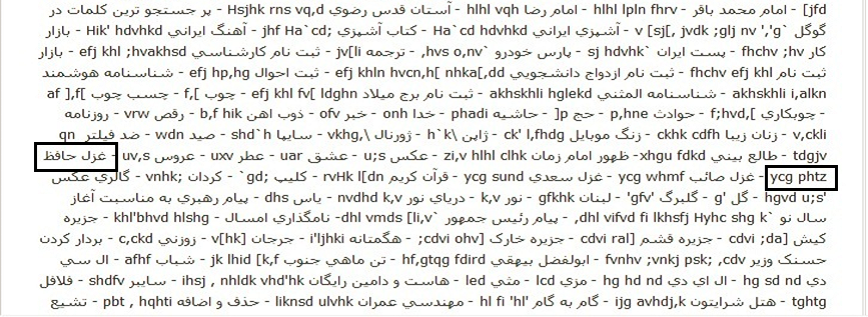
\includegraphics[scale=0.7]{Figures/plot2.png}
\caption{\label{fig:plot2}
رفتار وب‌گاه‌های فارسی به ازای مقادیر مختلف ویژگی «تعداد منابع چندرسانه‌ای»
}
\end{figure}
\item
تعداد \lr{i-frame}های درون هر صفحه: استفاده از \lr{i-frame}ها در وب‌گاه‌های هرز فارسی امری رایج است که به هرزنویسان کمک می‌کند تا بتوانند بخش‌هایی از صفحه یا صفحات دیگر را درون صفحه خود نمایش دهند. این صفحات معمولا با استفاده از تعداد زیادی کلیدواژه درون ابربرچسب یا به صورت پنهان درون بدنه صفحه، کاربران را به سمت صفحه خود هدایت می‌کنند. سپس با استفاده از مطالب نامرتبط موجود در صفحات دیگر، مدت زمان ماندن کاربران را در صفحه خود افزایش می‌دهند. همچنین تعدادی از این صفحات، رونوشتی از پیوندهای موجود در صفحات دیگر را درون \lr{i-frame}‌ها قرار داده و با استفاده از این پیوندها کاربران را به سمت سایر صفحات هرز هدایت می‌کنند. نمودار \ref{fig:plot3} نشان می‌دهد که صفحاتی که از \lr{i-frame}های بیشتری استفاده کرده‌اند با احتمال بیشتری هرز می‌باشند.
\begin{figure}
\centering
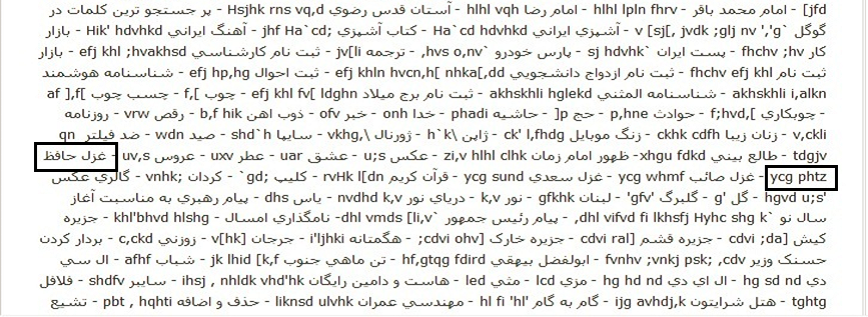
\includegraphics[scale=0.7]{Figures/plot3.png}
\caption{\label{fig:plot3}
رفتار وب‌گاه‌های فارسی به ازای مقادیر مختلف ویژگی «تعداد \lr{i-frame}ها»
}
\end{figure}
\item
درصدی از صفحه که از ایست‌واژه‌ها تشکیل شده است: این ویژگی در واقع مدل بهبود یافته‌ای از ویژگی «تعداد ایست‌واژه‌ها در هر صفحه» می‌باشد. همان‌طور که در بخش مربوط به مجموعه ویژگی‌های مکمل توضیح داده شد، به دلیل اختلاف طول صفحات با یکدیگر، محاسبه تعداد کل ایست‌واژه‌های هر صفحه برای شناسایی وب‌گاه‌های هرز کاربرد چندانی ندارد. بنابراین در این پژوهش ویژگی دیگری را ارائه می‌دهیم که برای محاسبه آن تعداد ایست‌واژه‌ها را بر تعداد کل کلمات موجود در صفحه تقسیم می‌نماییم. این امر باعث می‌شود خطاهایی که به دلیل یکسان نبودن طول صفحات وب ایجاد می‌شود تا حدود زیادی کاهش یابد. با توجه به نمودار \ref{fig:plot4} مشاهده می‌کنیم که احتمال هرز بودن وب‌گاه‌های فارسی، با کاهش تعداد ایست‌واژه‌ها افزایش می‌یابد. دلیل این امر وجود وب‌گاه‌های هرزی است که با استفاده از تعداد زیادی کلیدواژه بدون وجود جمله‌های معنادار ایجاد شده‌اند. 
\begin{figure}
\centering
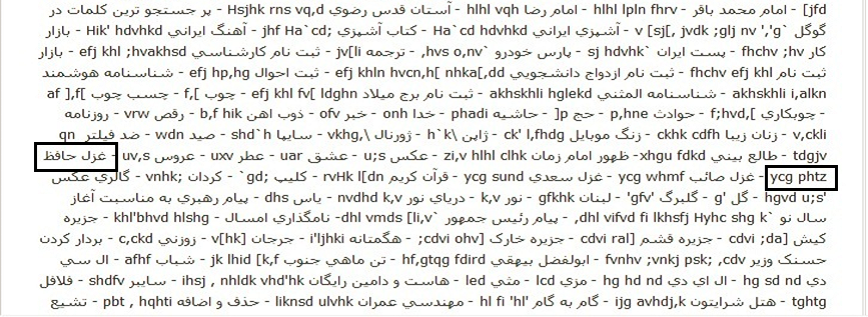
\includegraphics[scale=0.7]{Figures/plot4.png}
\caption{\label{fig:plot4}
رفتار وب‌گاه‌های فارسی به ازای مقادیر مختلف ویژگی «درصدی از صفحه که شامل ایست‌واژه است» 
}
\end{figure}
\item
درصدی از ایست‌واژه‌ها که درون صفحه استفاده شده است: این ویژگی به عنوان مکملی برای ویژگی قبل می‌باشد. هرزنویسان می‌توانند برای فریب روش قبل، تعداد کمی از ایست‌واژه‌ها را به دفعات زیاد درون صفحه خود تکرار کنند. همچنین وجود این ویژگی باعث می‌شود آن بخش از خطاهایی که به علت وجود تفاوت در طول صفحات ایجاد می‌شود از بین برود. برای مثال در صورتی که یک صفحه وب تنها از سه کلمه تشکیل شده باشد و دو کلمه آن جزء ایست‌واژه‌ها باشد، مقدار ویژگی قبل برای این صفحه ٪۶۷ محاسبه می‌شود. در صورتی که  درصد ایست‌واژه‌های یکتا در این صفحه نشان می‌دهد که تعداد ایست‌واژه‌های یکتای موجود در این صفحه زیاد نمی‌باشد. نمودار \ref{fig:plot5} نمایان‌گر نحوه توزیع وب‌گاه‌های فارسی بر روی مقادیر مختلف این ویژگی و همچنین احتمال هرز بودن این وب‌گاه‌‌ها می‌باشد. با توجه به نمودار، وب‌گاه‌هایی که تعداد ایست‌واژه‌های یکتا در آن‌ها کمتر است، با احتمال بیشتری هرز می‌باشند.
\begin{figure}
\centering
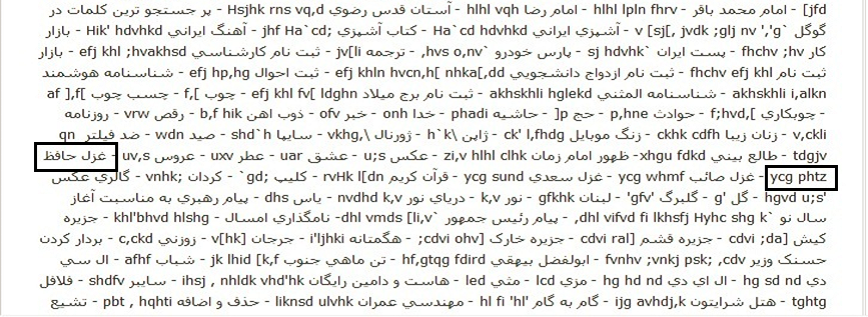
\includegraphics[scale=0.7]{Figures/plot5.png}
\caption{\label{fig:plot5}
رفتار وب‌گاه‌های فارسی به ازای مقادیر مختلف ویژگی «درصد ایست‌واژه‌ها»
}
\end{figure}
\item
شباهت کسینوسی بین ابربرچسب‌ها و محتوای قابل مشاهده هر صفحه: با توجه به این‌که برخی از موتورهای جست‌و‌جو به کلمات درون ابربرچسب‌ها وزن زیادی می‌دهند، بسیاری از هرزنویسان این بخش از صفحات خود را با تعداد زیادی کلیدواژه پر می‌کنند، که در این میان بسیاری از آن‌ها با موضوع و محتوای صفحه نامرتبط هستند. با محاسبه شباهت کسینوسی بین این ابربرچسب‌ها و محتوای قابل مشاهده توسط کاربر و در نظر گرفتن این معیار به عنوان یک ویژگی در رده‌بندی وب‌گاه‌ها می‌توانیم این نوع از وب‌گاه‌های هرز را تشخیص دهیم. همان‌طور که در نمودار \ref{fig:plot6} مشاهده می‌نماییم، مقدار شباهت کسینوسی در صفحات معتبر حدود ۰/۵ بوده و به هر میزان که مقدار این معیار از ۰/۵ کمتر یا بیشتر می‌شود، احتمال هرز بودن وب‌گاه‌‌های فارسی نیز افزایش می‌یابد. کاهش این شباهت نشان‌گر وب‌گاه‌های هرزی است که برای مرتبط کردن محتوای وب‌گاه خود با تعداد زیادی از پرس‌وجو‌ها، از کلیدواژه‌های مختلفی در صفحاتشان استفاده می‌کنند. همچنین افزایش این شباهت نشان‌دهنده وب‌گاه‌های هرزی است که برای بالا بردن وزن خود به ازای پرس‌وجوهای مشخص، مجموعه‌ای از کلیدواژه‌های مرتبط را به تعداد زیاد درون صفحات خود تکرار می‌کنند.
\begin{figure}
\centering
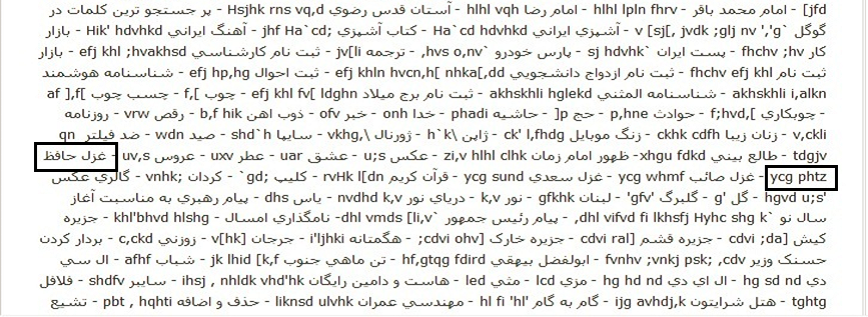
\includegraphics[scale=0.7]{Figures/plot6.png}
\caption{\label{fig:plot6}
رفتار وب‌گاه‌های فارسی به ازای مقادیر مختلف «شباهت کسینوسی بین ابربرچسب‌ها و محتوای قابل مشاهده صفحه» 
}
\end{figure}
\item
میزان ابربرچسب‌های جاوا‌ اسکریپت در هر صفحه: کدهای جاوا اسکریپت معمولا زمانی اجرا می‌شوند که رخدادی به وقوع می‌پیوندد. هرزنویسان معمولا با استفاده از کدهای جاوا اسکریپت، برخی رخدادهای پویا را کنترل می‌کنند. برای مثال زمانی که وارد یک صفحه هرز می‌شویم یا زمانی که روی یک پیوند درون صفحه تلیک می‌نماییم، تعدادی صفحه (معمولا تبلیغاتی) به طور خودکار توسط مرورگر نمایش داده می‌شود. در برخی مواقع نیز قبل از نمایش صفحه، کاربران به طور خودکار به صفحه دیگری هدایت می‌شوند. نمودار \ref{fig:plot7} رشد صعودی احتمال هرز بودن صفحات را به ازای افزایش مقدار این ویژگی نشان می‌دهد.
\begin{figure}
\centering
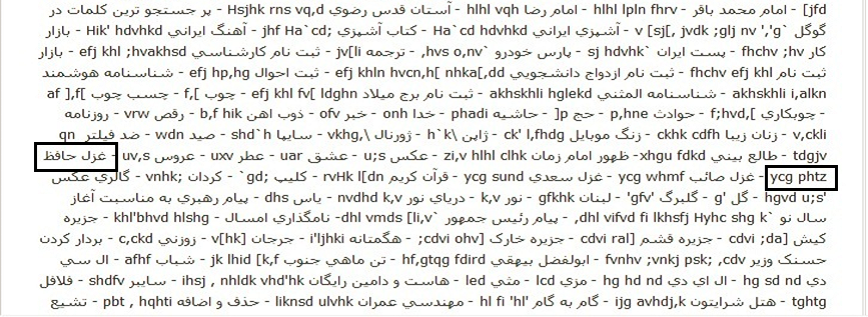
\includegraphics[scale=0.7]{Figures/plot7.png}
\caption{\label{fig:plot7}
رفتار وب‌گاه‌های فارسی به ازای مقادیر مختلف ویژگی «میزان ابربرچسب‌های جاوا اسکریپت» 
}
\end{figure}
\end{itemize}

\subsubsection{انتخاب ویژگی و رده‌بندی}
%\label{section:methodology-featureselectionclassification}
پس از استخراج هر دسته از ویژگی‌ها و بررسی رفتار آن‌‌ها در شناسایی هرز وب فارسی، برای مشخص کردن بهترین ویژگی‌ها و بهبود دقت رده‌بندی، از روش انتخاب ویژگی \lr{-test} $\chi^2$ استفاده نمودیم. در این روش میزان وابستگی هر یک از ویژگی‌ها با دو کلاس هرز و معتبر محاسبه شده و سپس ویژگی‌ها بر اساس امتیازی که بدست می‌آورند به صورت نزولی مرتب می‌شوند. هر چقدر یک ویژگی امتیاز بیشتری بدست آورد، بدین معنا می‌باشد که میزان وابستگی آن ویژگی به کلاس‌های تعریف شده بیشتر است و درنتیجه انتظار می‌رود که آن ویژگی بتواند کلاس نمونه‌ها را درست‌تر تشخیص دهد. در نهایت با استفاده از روش حذف پس‌رو، مجموعه‌ای از ویژگی‌ها را به عنوان ویژگی‌های بهینه انتخاب نمودیم. در این روش ابتدا با استفاده از تمام ویژگی‌های استخراج شده وب‌گاه‌ها را رده‌بندی کرده، سپس در هر مرحله ویژگی با کمترین امتیاز را حذف می‌نماییم. در صورتی که حذف یک ویژگی باعث کاهش کارایی رده‌بندی شود، آن ویژگی را مجددا به مجموعه ویژگی‌های بهینه اضافه می‌نماییم.
پس از حذف ویژگی‌های غیر‌بهینه، برای پیش‌بینی برچسب وب‌گاه‌ها، انواع الگوریتم‌های یادگیری ماشین مانند درخت تصمیم \lr{C4.5}، جنگل تصادفی، شبکه‌های عصبی، الگوریتم‌های بیزین، \lr{SVM} و $k$ نزدیک‌ترین همسایه را بررسی کرده و در نهایت، روش جنگل تصادفی را به دلیل کارایی بالاتر آن برای شناسایی وب‌گاه‌های هرز انتخاب نمودیم. همچنین، برای بررسی میران تاثیر هر ویژگی به طور مجزا در کارایی رده‌بند، فرآیند رده‌بندی را با استفاده از هر یک از ویژگی‌های بهینه به صورت مجزا انجام داده و دقت شناسایی وب‌گاه‌های هرز را برای آن محاسبه نمودیم.

\subsection{ارائه یک سامانه شناساگر هرز وب فارسی به نام \lr{PSD-SYS}}
\label{section:methodology-bosw}
در این بخش یک سامانه جدید به نام \lr{PSD-SYS}‌\LTRfootnote{Persian Web Spam Detection System} را ارائه می‌دهیم که در آن از مدل جدیدی به نام \lr{BOSW} برای استخراج ویژگی‌ها و همچنین روش انتخاب ویژگی بر اساس تعداد رخداد کلمات استفاده می‌شود. در این سامانه از الگوریتم \lr{SVM} برای رده‌بندی وب‌گاه‌ها استفاده می‌شود. در ادامه به توضیح دقیق‌تر درباره این سامانه و روش کار آن می‌پردازیم.

پس از بررسی تعداد زیادی از ویژگی‌های محتوایی بر روی وب‌گاه‌‌های فارسی، در این مرحله از پژوهش از یک شناساگر جدید هرز وب فارسی برای رده‌بندی وب‌گاه‌ها استفاده نمودیم. در این سامانه پس از انجام فرآیندهای پیش‌پردازش داده مانند حذف ابربرچسب‌های \lr{HTML} و حذف ایست‌واژه‌ها، از مدل جدیدی به نام \lr{BOSW} برای استخراج ویژگی‌ها استفاده می‌شود. مدل \lr{BOSW} در واقع مدل تغییر یافته‌ای از مدل ساده کیف کلمات است که اولین بار توسط \lr{Harris} \cite{harris1954distributional} استفاده شد و بعدها نیز در زمینه‌های پردازش زبان طبیعی و بازیابی اطلاعات موارد استفاده بسیاری پیدا کرد. در مدل کیف کلمات هر سند به صورت مجموعه‌ای از  $n$-گرام‌های یکتا نمایش داده می‌شود. با استفاده از این روش بسیاری از اطلاعات اضافی متن مانند \lr{POS}‌\LTRfootnote{Part of Speech}، ترتیب کلمات و سایر اطلاعات مربوط به جمله‌بندی متن حذف می‌شود. یکی از موارد استفاده مدل کیف کلمات در رده‌بندی اسناد است. بدین منظور تمام  $n$-گرام‌های یکتای موجود در کل مجموعه اسناد استخراج شده و به عنوان مجموعه‌ ویژگی‌ها در نظر گرفته می‌شوند. سپس هر سند به صورت برداری از این ویژگی‌ها نمایش داده می‌شود که می‌تواند به صورت دودویی یا وزن‌دار مقدار‌دهی شود. در روش دودویی، در صورتی که  $n$-گرام موردنظر در سند وجود داشته باشد درایه نظیر آن مقدار یک و در غیر این صورت مقدار صفر می‌گیرد. در روش وزن‌دار نیز از مدل‌های وزن‌دهی متفاوتی استفاده می‌شود که رایج‌ترین آن‌ها وزن‌دهی \lr{TF} یا \lr{TF-IDF} می‌باشد. 

با توجه به آزمایشی که بر روی وب‌گاه‌های فارسی انجام دادیم، به این نتیجه رسیدیم که استفاده از مدل ساده کیف کلمات در شناسایی وب‌گاه‌های هرز فارسی کارایی خوبی ندارد. این امر به دلیل وجود خطاهایی است که از کلمات موجود در وب‌گاه‌های معتبر ایجاد می‌شود. برخلاف صفحات وب هرز که معمولا دارای موضوع‌های مشابهی مانند موضوعات تبلیغاتی و تجاری هستند، صفحات معتبر بسته به کاربردشان دارای موضوع‌های متفاوتی می‌باشند. بنابراین، انتظار می‌رود انتخاب مجموعه کلمات رایج در صفحات هرز به عنوان بردار ویژگی، در شناسایی وب‌گاه‌های هرز تاثیر بسزایی داشته باشد. این کلمات معمولا با ترکیب خاصی در صفحات هرز ظاهر می‌شوند. در صورتی که اگر کلمات رایج در وب‌گاه‌های معتبر را نیز در بردار ویژگی در نظر بگیریم، علاوه بر افزایش هزینه محاسباتی، در مواردی نیز ممکن است باعث کاهش خطای رده‌بندی شود.  

برای حل مشکلات مطرح شده، در \lr{PSD-SYS} از مدل \lr{BOSW} استفاده شده است. در این مدل به جای استخراج $n$-گرام‌های یکتا از کل مجموعه اسناد موجود در پیکره، ابتدا مجموعه وب‌گاه‌های هرز را جدا کرده و سپس $n$-گرام‌های یکتای موجود در آن‌ها را استخراج می‌کنیم و به عنوان مجموعه ویژگی‌ها در نظر می‌گیریم. سپس هر صفحه وب به صورت برداری از ویژگی‌های مشخص شده نمایش داده می شود. همان‌طور که توضیح دادیم بردار ویژگی می‌تواند با استفاده از روش‌های وزن‌دهی متفاوتی مقداردهی شود که در این سامانه پس از آزمایش روش‌های وزن‌دهی مختلف، در نهایت از روش دودویی که بهترین نتیجه را داده است استفاده می‌شود.

برای کاهش زمان پردازش و همچنین بهبود کارایی رده‌بندی نهایی، در \lr{PSD-SYS} از  روش‌های مختلف انتخاب ویژگی مانند \lr{-test}$\chi^2$، \lr{mutual information} ، \lr{TF} و \lr{TF-IDF} برای ۱-گرام و ۲-گرام‌ها، استفاده کردیم. به ازای هر روش، ویژگی‌هایی را که امتیازشان از آستانه تعیین شده بیشتر بود به عنوان مجموعه ویژگی‌های مناسب برای رده‌بندی در نظر گرفته و بقیه ویژگی‌ها را حذف کردیم. در نهایت برای رده‌بندی وب‌گاه‌ها از الگوریتم \lr{SVM} به دلیل کارایی بالاتر آن نسبت به سایر الگوریتم‌های یادگیری ماشین استفاده کردیم. نتایج آزمایش‌ها در بخش \ref{subsubsection:experiments-results-content-psdsys} نشان می‌دهد که این سامانه شناساگر هرز وب فارسی نسبت به سایر روش‌های شناسایی هرز وب محتوایی دقت و فراخوانی بالاتری دارد.

\section{الگوریتم‌های مبتنی بر پیوند برای شناسایی هرز وب}
\label{chapter:ٍlinkbased}
در این بخش از پژوهش الگوریتم‌هایی را پیشنهاد می‌دهیم که با استفاده از آن‌ها می‌توان با داشتن برچسب اعتبار  (هرز) مجموعه محدودی از وب‌گاه‌ها و با بهره‌گیری از ساختار گرافی وب، امتیاز ارزشمندی  (هرز بودن) سایر وب‌گاه‌ها را محاسبه کرد. 

اساس کار روش‌های پیشنهادی در این بخش، الگوریتم‌های انتشار برچسب  مانند \lr{TrustRank} و   \lr{Anti-TrustRank} هستند که به صورت نیمه‌سرپرست و با داشتن امتیاز تعدادی از گره‌های درون گراف، امتیاز سایر گره‌های گراف را محاسبه می‌کنند. برای استفاده از روش‌های انتشار برچسب در حل مسائل مختلف، ابتدا باید مسئله را به صورت یک گراف مدل‌سازی کرد. بنابراین در این بخش، ابتدا به توضیح مختصری درباره نحوه مدل‌سازی گراف وب می‌پردازیم. سپس در بخش \ref{section:linkbased-wp}، الگوریتمی به نام \lr{WorthyRank} را معرفی می‌کنیم که با شروع از یک مجموعه بذر معتبر اولیه با امتیاز ارزشمندی مشخص، به صورت پیش‌رو امتیاز ارزشمندی آن‌ها را در کل گراف انتشار داده و در نهایت وب‌گاه‌ها را بر اساس امتیاز ارزشمندی نهایی که بدست می‌آورند رتبه‌بندی می‌کند. در این الگوریتم با استفاده از روش‌هایی مانند انتخاب بهینه گره‌های بذر، وزن‌دهی به یال‌‌های گراف و همچنین بسط دوره‌ای گره‌های بذر، برخی از مشکلاتی که در الگوریتم‌های انتشار برچسب پیشین وجود دارد برطرف می‌شود. در بخش \ref{section:linkbased-twsp} نیز الگوریتمی به نام \lr{JunkyRank} را پیشنهاد می‌دهیم که با داشتن مجموعه‌ای از وب‌گاه‌های هرز به عنوان بذر اولیه، امتیاز هرز بودن آن‌ها را هم‌زمان به صورت پس‌رو و پیش‌رو در کل گراف انتشار داده و پس از ترکیب خطی این امتیازها با امتیازهای ارزشمندی وب‌گاه‌ها که با استفاده از الگوریتم \lr{WorthyRank} محاسبه شده است، در نهایت وب‌گاه‌ها را بر اساس امتیاز هرز بودنشان رتبه‌بندی می‌کند. 
\subsection{مدل‌سازی گراف وب}
\label{section:linkbased-graphmodeling}  
برای استفاده از اطلاعات مربوط به ساختار پیوندی بین صفحات وب ابتدا باید صفحات وب و پیوندهای بین آن‌ها را به صورت یک گراف مدل‌سازی کرد. با فرض وجود $N$ وب‌گاه، گراف جهت‌دار G دارای $N$ گره با مشخصه‌های ۱، ۲، ۳، ...، $n$ است که با استفاده از یال‌های جهت‌دار به یکدیگر متصل هستند. در صورتی که $A$ ماتریس مجاورت این گراف باشد به ازای هر زوج گره $(i,j)$، اگر از وب‌گاه $i$ به یکی از صفحات وب‌گاه $j$ پیوندی وجود داشته باشد مقدار $a_{ij}$ برابر با یک و در غیر این صورت این مقدار برابر با صفر است. در صورت وزن‌دار بودن گراف، وزن هر یال، نشان‌دهنده تعداد پیوندهای صفحات درون وب‌گاه مبدا به صفحه یا صفحاتی در وب‌گاه مقصد می‌باشد.

\subsection{الگوریتم \lr{WorthyRank}}
\label{section:linkbased-wp}
با بررسی رفتار صفحات وب در اینترنت مشاهده می‌شود که تعداد زیادی از ارجاع‌های درون یک وب‌گاه معتبر، به صفحات معتبر دیگر می‌باشد \cite{gyongyi2004combating}. یک وب‌گاه معتبر، با توجه به این‌که دارای مطالب مفید و معتبر می‌باشد، پیوندهای درون آن نیز که مرتبط با مطالب درون صفحه هستند، پیوندهای معتبری بوده که به سایر صفحات  معتبر اشاره می‌کنند. بنابراین در گراف وب، با داشتن امتیاز یک گره معتبر، می‌توان بخشی از این امتیاز را به گره‌های همسایه خروجی از آن گره انتقال داد.

با در نظر گرفتن این مهم، در این بخش الگوریتم نیمه‌سرپرستی را معرفی می‌نماییم که با داشتن تعداد اندکی وب‌گاه معتبر به عنوان بذر، و وزن‌دهی اولیه به آن‌ها، میزان امتیاز ارزشمندی آن‌ها را به صورت پیش‌رو در کل گراف انتشار می‌دهد. در روش پیش‌رو، امتیاز یک گره طبق قاعده مشخصی بین گره‌های مقصد یال‌های خروجی آن گره تقسیم می‌شود. 
%مشکلی که در روش انتشار امتیاز اعتبار به صورت پیش‌رو وجود دارد، وجود پیوندهای جعلی بین صفحات وب است. دلیل وجود این پیوندها، وب‌گاه‌های هرزی هستند که پیوند مربوط به صفحه خود را درون بخش‌هایی از وب‌گاه‌های معتبر قرار می‌دهند. برای مثال، 
همچنین با توجه به این‌که برچسب گره‌های بذر مشخص است، این گره‌ها همواره یک وزن مشخصی از امتیاز اولیه خود را دریافت می‌کنند. این الگوریتم به صورت دوره‌ای تا زمانی تکرار می‌شود که میزان تغییر امتیاز هر وب‌گاه‌ در دو دور متوالی کمتر از $\epsilon$ باشد. 

در نهایت تمام وب‌گاه‌ها به ترتیب بر اساس بیشترین میزان امتیاز ارزشمندی، رتبه‌بندی می‌شوند. هدف از این الگوریتم این است که وب‌گاه‌های معتبر در رتبه‌های بالاتر و وب‌گاه‌های هرز در رتبه‌های پایین‌تر  قرار بگیرند. یکی از کاربردهای اصلی این الگوریتم می‌تواند در موتورهای جست‌و‌جو باشد. هدف موتورهای جست‌و‌جو این است که با استفاده از الگوریتم‌های مختلف، صفحات وب را به ترتیب بر اساس میزان اعتبار و ارتباطشان با پرس‌وجوی موردنظر به کاربر پیشنهاد دهند. در این وظیفه، هر چقدر تعداد صفحات هرز در میان نتایج جستجو کمتر باشد، رضایت کاربران از موتور جست‌وجو بیشتر می‌شود. شکل \ref{fig:worthy} مراحل اجرای الگوریتم \lr{WorthyRank} را نشان می‌دهد. مطابق این شکل، این الگوریتم چند بخش اصلی دارد که در ادامه به شرح هر یک از آن‌ها می‌پردازیم.
\begin{figure}
\centering
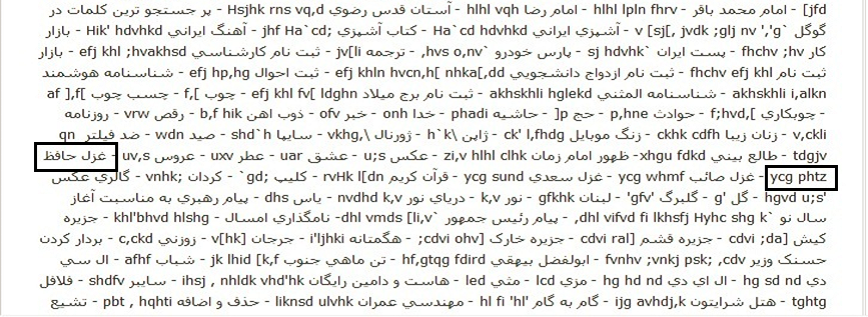
\includegraphics[scale=0.65]{Figures/worthy.png}
\caption{\label{fig:worthy}
مراحل اجرای الگوریتم \lr{WorthyRank} 
}
\end{figure}


\subsubsection{انتخاب و وزن‌دهی گره‌های بذر}
\label{section:linkbased-wp-seedweighting}
همان‌طور که در بخش \ref{section:relatedwork-link} توضیح دادیم، روش انتخاب بذر در دقت نهایی الگوریتم‌های انتشار برچسب موثر می‌باشد. در این پژوهش برای کاهش خطای ناشی از انتخاب بذر از الگوریتم \lr{PageRank} \mls{معکوس} استفاده می‌نماییم. این الگوریتم مانند الگوریتم \lr{PageRank} است با این تفاوت که برای محاسبه امتیاز گره‌ها، ابتدا جهت یال‌های گراف معکوس می‌شود. همان‌طور که در \cite{gyongyi2004combating} نیز توضیح داده شده است، با استفاده از این الگوریتم می‌توان گره‌هایی را که بیشترین توانایی انتشار امتیار اعتماد در کل گراف را دارند مشخص کرد. پس از محاسبه \lr{PageRank} معکوس برای تمام گره‌های درون گراف، آن‌ها را به ترتیب  به صورت نزولی بر اساس این امتیاز مرتب کرده و شروع به برچسب‌گذاری آن‌ها می‌نماییم. این کار را تا زمانی ادامه می‌دهیم که مقدار گره‌های معتبر، به تعداد موردنظر رسیده باشد.
با استفاده از این روش در نهایت  مجموعه‌ای از $L^+$ وب‌گاه‌ برچسب‌خورده معتبر داریم. با در نظر گرفتن وب‌گاه‌های بذر، بردار  $\vec{S} = (s_1, s_2, ..., s_n)$ را بدست می‌آوریم که در آن $s_i$ طبق رابطه \ref{eq:goodseed} محاسبه می‌شود.
\begin{equation}
\label{eq:goodseed}
  s_i =\begin{cases}
     \frac{1}{L^+} ,& \text{if} \; \;  i \in S^+\\
    0, & \text{otherwise}
  \end{cases}
\end{equation}

\subsubsection{وزن‌دهی یال‌های گراف}
\label{section:linkbased-wp-linkweight}
یکی از مشکلاتی که در گراف‌ وب وجود دارد، وجود پیوندهای جعلی بین صفحات و وب‌گاه‌های مختلف می‌باشد. دلیل این امر هرزنویسانی هستند که برای افزایش رتبه وب‌گاه‌های هرز خود، پیوند صفحاتشان را درون وب‌گاه‌های معتبری قرار می‌دهند که به کاربران امکان نوشتن نظرات و یا مطالب دلخواه دیگر را درون بخش‌هایی از صفحات خود می‌دهند. در این پژوهش برای حل این مشکل از \mls{ضریب جاکارد} برای محاسبه میزان اعتبار پیوندهای موجود در گراف وب استفاده می‌کنیم. با استفاده از این ضریب، ماتریس مجاورت $A$ را به ماتریس وزن‌دار $M$ تبدیل می‌کنیم که در آن $0 \leq m_{ij} \leq 1$ وزن اعتبار پیوند بین دو وب‌گاه $i$ و $j$ است که به صورت زیر محاسبه می‌شود:
 \begin{equation}
	m_{ij} = \frac{|N(i)\cap N(j)|}{|N(i)\cup N(j)|}
	\label{Eq:jac}
\end{equation}
که در آن $N(i)$ مجموعه تمام همسایه‌های گره $i$ است. با توجه به رابطه \ref{Eq:jac} امتیازی که با استفاده از این روش به پیوند بین دو وب‌گاه داده می‌شود بر اساس میزان اشتراک همسایه‌های دو وب‌گاه است. پیوند بین دو وب‌گاه نمایان‌گر وجود یک ارتباط بین دو وب‌گاه است. در نتیجه در صورتی که این ارتباط واقعی باشد احتمال وجود اشتراک بین همسایه‌های این دو وب‌گاه نیز زیاد است. بنابراین با استفاده از این روش یال‌های گراف اعتبارسنجی شده و یال‌های مربوط به پیوندهای جعلی که توسط هرزنویسان درون صفحات مختلف قرار داده شده است وزن کمی می‌گیرند. 

%برای مثال همان‌طور که در شکل ؟؟ مشاهده می‌کنیم در صورتی که برای انتشار وزن هر گره از تمام یال‌های آن استفاده کینم
%همچنین لازم به ذکر است که برخلاف بسیاری از روش‌های پیشین، در این الگوریتم وزن یال‌ها نرمال‌سازی نمی‌شود. دلیل این امر

\subsubsection{انتشار امتیاز ارزشمندی}
\label{section:linkbased-wp-wpropagation}
پس از مشخص کردن مجموعه گره‌های بذر و وزن‌دهی آن‌ها، در هر تکرار $t$، امتیاز ارزشمندی گره $i$ به صورت زیر محاسبه می‌شود:
 \begin{equation}
	r_{i}(t) = \alpha \sum\limits_{j=1}^n m_{ji} r_{j}(t-1) + (1-{\alpha}) * s_i
	\label{Eq:worthprop}
\end{equation}
در این رابطه $\alpha$ یک \mls{عامل میرایی} است که مشخص می‌کند چند درصد از امتیاز ارزشمندی هر صفحه از امتیاز سایر صفحاتی که به آن ارجاع داده‌اند و چند درصد آن، از مقدار وزن مشخصی که به صفحات بذر داده می‌شود تامین شود. همچنین مقدار $s_i$ همان مقدار مربوط به وزن اولیه صفحات بذر است که با استفاده از رابطه \ref{eq:goodseed}  محاسبه شده است.
 
\subsubsection{بسط دوره‌ای گره‌های بذر}
\label{section:linkbased-wp-seedexpansion}
همان‌طور که در بخش \ref{section:relatedwork-link} توضیح دادیم، در پژوهش‌هایی که بر روی تاثیر اندازه مجموعه گره‌های بذر بر روی نتیجه نهایی الگوریتم‌های انتشار امتیاز مانند \lr{TrustRank} \cite{gyongyi2004combating} انجام شده است، نشان داده‌اند که کم بودن تعداد بذرهای اولیه می‌تواند باعث کاهش دقت رتبه‌بندی نهایی شود. از طرف دیگر برچسب‌گذاری وب‌گاه‌ها به طور دستی کاری بسیار زمان‌بر و پرهزینه می‌باشد. بنابراین در الگوریتم \lr{WorthyRank} از روش جدیدی به نام بسط دوره‌ای بذر استفاده می‌کنیم که با داشتن تعداد کمی بذر اولیه، در هر مرحله تعداد وب‌گاه‌های بذر را به طور خودکار افزایش می‌دهد. در این روش ابتدا تعداد محدودی از گره‌های معتبر را به عنوان گره‌های بذر انتخاب می‌نماییم. سپس در هر بار تکرار الگوریتم، امتیاز اعتماد گره‌ها را محاسبه کرده و آ‌ن‌ها را به صورت نزولی مرتب می‌نماییم. سپس $k$ گره با بیشترین امتیاز ارزشمندی را به عنوان بذرهای جدید به مجموعه بذر اولیه اضافه می‌کنیم. این کار را تا جایی ادامه می‌دهیم که تعداد گره‌های بذر به $f$ درصد تعداد کل گره‌های گراف برسد.

\subsection{الگوریتم \lr{JunkyRank}}
\label{section:linkbased-twsp}
الگوریتم‌های انتشار برچسب هرز مانند \lr{Anti-TrustRank} \cite{krishnan2006web}، \lr{DRank} \cite{zhang2011propagating} و \lr{BRank} \cite{liu2013combating} بر اساس این فرض عمل می‌کنند که صفحاتی که به یک صفحه هرز ارجاع می‌دهند به احتمال زیاد جزء صفحات هرز می‌باشند. بر این اساس، در این الگوریتم‌ها امتیاز هرز بودن هر صفحه در مسیر عکس جهت یال‌های گراف به تمام صفحاتی که به آن صفحه ارجاع داده‌اند انتشار داده می‌شود. مشکلی که در این دسته از الگوریتم‌ها وجود دارد این است که هیچ احتمال هرز بودنی برای صفحاتی که یک صفحه هرز به آن‌ها ارجاع داده است در نظر گرفته نمی‌شود. این امر در حالی است که تعداد زیادی از صفحات هرز برای افزایش رتبه‌شان، به یکدیگر ارجاع می‌دهند. این‌گونه از صفحات که معمولا بخشی از یک دهکده‌پیوندی هستند، با تبادل پیوند با یکدیگر، رتبه وب‌گاه‌های خود را نسبت به سایر وب‌گاه‌ها افزایش می‌دهند. 

برای مثال در شکل \ref{fig:linkfarm} که بخشی از یک گراف وب را نشان می‌دهد، مجموعه گره‌های ۳، ۴، ۵، ۶ و ۷، با یکدیگر یک دهکده پیوندی را تشکیل می‌دهند. در این گراف، گره‌های سفید مربوط به وب‌گاه‌های معتبر و گره‌های خاکستری نشان‌گر وب‌گاه‌های هرز می‌باشند. با انتخاب گره‌های ۴ و ۶ به عنوان بذر هرز، در صورتی که برای محاسبه امتیاز هرز سایر گره‌ها، فقط از انتشار امتیاز در مسیر یال‌های گراف استفاده شود، گره ۷ هیچ امتیاز هرزی دریافت نمی‌کند. 
%این امر در حالی است که یکی از هدف‌های تشکیل دهکده‌ پیوندی در این گراف، افزایش  رتبه گره ۷ می‌باشد. 
با توجه به این‌که در الگویتم \lr{JunkyRank} امتیاز هرز گره‌های بذر به صورت پیش‌رو نیز در گراف انتشار داده می‌شود، گره ۷ در رتبه‌بندی بر اساس امتیاز هرز توسط این الگوریتم، در رتبه‌های بالاتر قرار می‌گیرد.

\begin{figure}
\centering
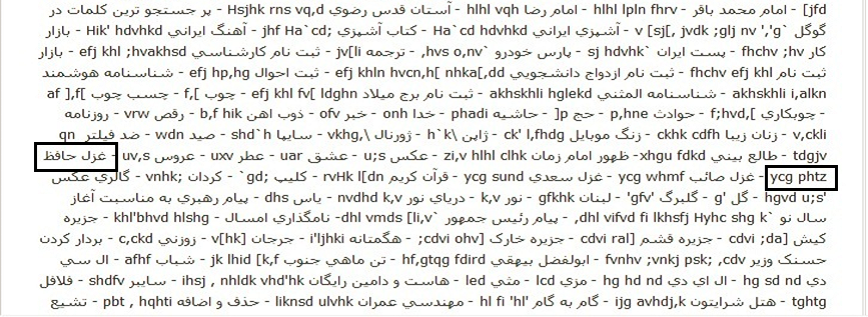
\includegraphics[scale=0.5]{Figures/linkfarm.png}
\caption{\label{fig:linkfarm}
بخشی از گراف وب که دارای یک دهکده پیوندی می‌باشد.
}
\end{figure}
برای حل این مشکل الگوریتمی به نام \lr{JunkyRank} را معرفی می‌نماییم که با داشتن مجموعه‌ای از وب‌گاه‌های هرز به عنوان بذر اولیه، امتیاز هرز بودن آن‌ها را هم‌زمان به دو صورت پیش‌رو و پس‌رو در گراف وب انتشار می‌دهد. این الگوریتم دو بخش اصلی دارد که در ادامه به شرح هر یک از آن‌ها می‌پردازیم.

\subsubsection{انتخاب و وزن‌دهی گره‌های بذر}
در این بخش برای انتخاب گره‌های بذر، از الگوریتم \lr{HITS} \cite{kleinberg1999authoritative} استفاده می‌نماییم. در این الگوریتم برای هر گره در گراف وب دو امتیاز محاسبه می‌شود. امتیاز \lr{hub} برای یک گره،  مشخص می‌کند که یک گره چه میزان  پیوند خروجی به گره‌های با \lr{authority} بالا دارد. همچنین امتیاز \lr{authoruty} نیز برای یک گره، نشان‌گر میزان ارجاعات گره‌های مختلف با امتیاز \lr{hub} بالا به آن گره می‌باشد. با توجه به این‌که امتیاز گره‌های بذر در الگوریتم \lr{JunkyRank}، هم به صورت هم‌جهت با یال‌های گراف و هم در خلاف جهت یال‌های گراف انتشار داده می‌شود، گره‌هایی به عنوان بذر مناسب هستند که  مقدار \lr{hub} و یا \lr{authority} بالایی داشته باشند. 

برای انتخاب گره‌های بذر در این الگوریتم، ابتدا الگوریتم \lr{HITS} را بر روی گراف وب اجرا می‌کنیم، سپس برای انتخاب $l$ گره به عنوان بذر، $\frac{l}{2}$ آن را از گره‌های با بیشترین امتیاز \lr{hub} و $\frac{l}{2}$ آن را از گره‌های با بیشترین امتیاز \lr{authorithy} انتخاب می‌نماییم. دلیل این امر، انتخاب گره‌هایی به عنوان بذر است که قابلیت بالایی را در انتشار امتیاز به صورت پیش‌رو و پس‌رو در کل گراف دارند. با استفاده از این روش در نهایت مجموعه‌ای از $l^-$ وب‌گاه‌ها برچسب‌خورده هرز داریم. با توجه به این مجموعه وب‌گاه‌های بذر، بردار $\vec{S^\prime} = (s^\prime_1, s^\prime_2, ..., s^\prime_n)$ را بدست می‌آوریم، به طوری‌که در آن، مقدار  $s^\prime_i$ طبق رابطه \ref{eq:badseed} محاسبه می‌شود.
\begin{equation}
\label{eq:badseed}
  s^\prime_i =\begin{cases}
     \frac{1}{L^-} ,& \text{if} \; \;  i \in S^-\\
    0, & \text{otherwise}
  \end{cases}
\end{equation}
% که $l^\prime$ تعداد وب‌گاه‌های هرز بذر و  $s^\prime_m$ وزن مربوط به بذر هرز $m$ام می‌باشد که مقدار آن برابر با $\frac{1}{l^\prime}$ است.

\subsubsection{انتشار امتیاز هرز بودن}

همان‌طور که توضیح دادیم، مزیت الگوریتم \lr{JunkyRank} نسبت به روش‌های پیشین این است که علاوه بر انتشار امتیاز هرز بودن در خلاف جهت یال‌ها، این امتیاز را در جهت یال‌های گراف وب نیز انتشار می‌دهد. نکته‌ای که باید در نظر داشت این است که  احتمال هرز بودن یک وب‌گاه، در صورتی که به یک وب‌گاه هرز ارجاع داده باشد، بیشتر از حالتی است که توسط یک وب‌گاه هرز ارجاع داده شده باشد. دلیل این امر این است که وب‌گاه‌های هرز در خیلی از موارد برای افزایش رتبه خود، به وب‌گاه‌های معتبر ارجاع می‌دهند. بنابراین برای کاهش اثر منفی وجود این نوع از پیوندهای جعلی در گراف وب، در این الگوریتم از ضریبی به نام $\beta$ استفاده می‌شود که به یال‌های ورودی به یک صفحه و یال‌های خروجی از آن وزن متفاوتی می‌دهد. 

رابطه \ref{eq:junky} نحوه محاسبه امتیاز هرز بودن وب‌گاه‌ها را در الگوریتم \lr{JunkyRank} نشان می‌دهد. با استفاده از ضریب $\beta$ در این رابطه، می‌توان بخش کمی از امتیاز هرز یک گره را در جهت یال‌های گراف و وزن بیشتری از آن را در خلاف جهت یال‌های آن گره انتشار داد.
\begin{equation}
r_{i}(t) = \alpha \left( {\beta \sum\limits_{j=1}^n a_{ij} r_{j}(t-1) + (1-{\beta})  \sum\limits_{j=1}^n a_{ji} r_{j}(t-1)} \right) + (1-{\alpha}) * {s^\prime}_i
	\label{eq:junky}
\end{equation}


پس از انتشار امتیاز هرز بودن گره‌‌های بذر در گراف و رسیدن به حالت \mls{همگرایی}، برای هر وب‌گاه یک امتیاز هرز بودن بدست می‌آید. اما استفاده از این امتیاز برای رده‌بندی وب‌گاه‌ها به تنهایی کافی نمی‌باشد. دلیل این امر وجود وب‌گاه‌های هرزی است که برای بالا بردن رتبه خود، پیوند تعداد زیادی از وب‌گاه‌های معتبر را درون صفحاتشان می‌گذارند. 

در صورتی که برای رتبه‌بندی نهایی وب‌گاه‌ها، فقط از امتیاز بدست آمده از الگوریتم \lr{JunkyRank} استفاده کنیم، امتیاز هرز بودن این‌گونه از وب‌گاه‌های معتبر که مورد هجوم وب‌گاه‌های هرز قرار گرفته‌اند بالا می‌رود. در صورتی که این امتیاز صحیح نمی‌باشد و برای مشخص کردن این امر کافی است که امتیاز ارزشمندی این‌گونه وب‌گاه‌های معتبر نیز محاسبه شود. 
در نتیجه، برای رتبه‌بندی این وب‌گاه‌ها بر اساس احتمال هرز بودن آن‌ها، ابتدا ترکیب خطی امتیاز هرز بودن وب‌گاه‌ها در الگوریتم \lr{JunkyRank} را با امتیاز ارزشمندی آن‌ها در الگوریتم \lr{WorthyRank} با استفاده از رابطه \ref{eq:lc} بدست آورده و در نهایت وب‌گاه‌ها را بر اساس امتیاز حاصله از این ترکیب خطی رتبه‌بندی می‌کنیم.
\begin{equation}
JunkyRank_{\gamma} = \gamma * JunkyRank - (1-{\gamma}) * WorthyRank
	\label{eq:lc}
\end{equation}

برای مثال در شکل \ref{fig:linkfarm}، در صورتی که برای شناسایی وب‌گاه‌های هرز، فقط امتیاز هرز بودن گره‌ها را در نظر بگیریم، گره‌های معتبر ۱ و ۸ و ۹ نیز به عنوان صفحات هرز شناسایی می‌شوند. در حالی‌که با انتخاب دو گره ۲ و ۱۰ به عنوان بذر معتبر و استفاده از ترکیب خطی امتیاز هرز با امتیاز اعتمادی که گره‌ها با استفاده از الگوریتم \lr{WorthyRank} کسب می‌کنند، می‌توان کیفیت رتبه‌بندی را بهبود داد.
\subsection{اثبات همگرایی}
\label{section:linkbased-convergence}
%در این بخش، برای اثبات همگرایی از برخی از روش‌های جبر خطی و قضایای مربوط به آن استفاده می‌کنیم.
برای اثبات همگرایی یک الگوریتم، ابتدا لازم است که شرط یا شرایطی را برای همگرایی آن تعریف نماییم. در الگوریتم‌های مبتنی بر پیوندی که در این پژوهش معرفی کرده‌ایم شرطی که برای همگرایی در نظر می‌گیریم به صورت رابطه \ref{eq:convcond} می‌باشد.
\begin{equation}
	\forall i : |r_i(t) - r_i(t-1)| \leq \epsilon    \Longleftrightarrow    \lim_{t \to \infty} \frac{r_i(t)}{r_i(t-1)} = 1
	\label{eq:convcond}
\end{equation}
طبق این رابطه، اجرای الگوریتم تا زمانی ادامه می‌یابد که مقدار اختلاف امتیاز هر گره، در دو دور متوالی از اجرای الگوریتم، کمتر از $\epsilon$ باشد. 

تمام الگوریتم‌هایی که در این بخش معرفی شده‌اند دارای یک پایه مشترک با یکدیگر هستند و آن میزان احتمالی است که وزن انتشار امتیاز از گره $i$ به گره $j$ را مشخص می‌کند و این‌که این وزن برخلاف بسیاری از روش‌های پیشین \mls{هنجارسازی} نمی‌شود. سایر سیاست‌‌های به‌کار گرفته شده در الگوریتم‌ها، مانند وزن‌دهی به گره‌های بذر، بسط مجموعه گره‌های بذر، وجود عامل میرایی و ترکیب خطی امتیاز ارزشمندی و غیر ارزشمندی تاثیری در همگرایی الگوریتم‌های انتشار برچسب ندارند. دلیل این امر این است که تمام موارد ذکر شده، به صورت یک پارامتر ثابت در روابط هر یک از الگوریتم‌ها ظاهر می‌شوند. تنها تاثیری که این پارامترها می‌توانند در الگوریتم‌های مربوطه داشته باشند، تاثیر آن‌‌ها در کارایی نهایی الگوریتم و همچنین زمان رسیدن به شرط همگرایی می‌باشد. با در نظر گرفتن این مهم، برای اثبات همگرایی الگوریتم‌های انتشار برچسب که در این بخش معرفی کرده‌ایم کافی است ثابت کنیم معادله ساده شده \ref{Eq:conv1} شرط همگرایی \ref{eq:convcond} را ارضا می‌کند. 
 \begin{equation}
r_{i}(t) = \sum\limits_{j=1}^n {m_{ji}} {r_{j}(t-1)}		
	\label{Eq:conv1}
\end{equation}

با تعریف بردار $R(t)=(r_1(t), r_2(t), ..., r_n(t))$ به عنوان بردار امتیاز صفحات در زمان $t$ که در آن $r_i(t)$ امتیاز وب‌گاه $i$ام در زمان $t$ است، می‌توان معادله \ref{Eq:conv1} را به صورت ماتریسی به صورت معادله \ref{Eq:conv2} نوشت. 
\begin{equation}
R(t) = {R(t-1)} {M}   \Longrightarrow   R(t) = {R(0)} {M^t}			
	\label{Eq:conv2}
\end{equation} 
طبق قضیه ۱-۵-۸ از کتاب \cite{horn2012matrix} برای یک ماتریس نامنفی و \mls{اصلی} $A$ داریم:
\begin{equation}
\lim_{m \to \infty}(\rho(A)^{-1} A)^m = L > 0
	\label{Eq:theorem}
\end{equation}
به طوری‌که $L=XY^T$، $AX=\rho(A)X$، $A^TY= \rho(A)Y$ و $X,Y>0$ است.

همچنین طبق قضیه ۲-۵-۸ در \cite{horn2012matrix}، یک ماتریس نامنفی $A$ یک ماتریس اصلی است اگر و تنها اگر $m\geq1$ وجود داشته باشد که به ازای آن داشته باشیم  $A^m>0$. با توجه به این‌که درایه‌های ماتریس مجاورت وزن‌دار $M$ در الگوریتم‌های معرفی شده، هر کدام مقداری بین ۰ و ۱ دارند، این ماتریس یک ماتریس نامنفی می‌باشد. همچنین با توجه به این‌که این ماتریس مربوط به گراف وب است و گراف وب یک گراف \mls{قویا متصل} است بنابراین به ازای هر زوج گره $i$ و $j$، حداقل یک مسیر از $i$ به $j$ وجود دارد. به عبارت دیگر $t\geq1$ وجود دارد به طوری‌که به ازای آن $M^t>0$ است. در نتیجه $M^t$ یک ماتریس اصلی است. بنابراین با توجه به معادله \ref{Eq:theorem} داریم:
\begin{equation}
\lim_{t \to \infty}(\lambda_1^{-1} M)^t = V_1 V_2^T   \Longrightarrow   M^t = \lambda_1^{t} V_1 V_2^T
	\label{Eq:conv7}
\end{equation}
با جایگذاری مقدار $M^t$ در رابطه \ref{Eq:conv2} داریم: 
\begin{equation}
R(t) = R(0) \lambda_1^{t} V_1{V_2^T}   \Longrightarrow   r_i(t) = \lambda_1^{t} \sum\limits_{k=1}^n {v_{1k}v_{2i} r_k(0)} 
	\label{Eq:conv10}
\end{equation}
در نتیجه برای شرط همگرایی \ref{eq:convcond} داریم:
\begin{equation}
\lim_{t \to \infty}\frac{r_i(t)}{r_i(t-1)} = \frac{\lambda_1^{t} \sum\limits_{k=1}^n {v_{1k} v_{2i} r_k(0)}}{\lambda_1^{t-1} \sum\limits_{k=1}^n {v_{1i} v_{2k} s_k(0)}} = \lambda_1 
	\label{Eq:conv15}
\end{equation}
با توجه به رابطه \ref{Eq:conv15} مشاهده می‌کنیم در صورتی‌ که امتیاز تمام گره‌ها پس از هر دور اجرای الگوریتم \mls{به‌هنجار} نشود، شرط همگرایی برقرار نمی‌شود. بنابراین پس از اعمال هنجار‌سازی امتیازها در رابطه \ref{Eq:conv15} داریم:
\begin{equation}
\lim_{t \to \infty}\frac{r_i(t)}{r_i(t-1)} = \frac{\left(\frac{\lambda_1^{t} \sum\limits_{k=1}^n {v_{1k} v_{2i} r_k(0)}} {\lambda_1^{t} \sum\limits_{i=1}^n \sum\limits_{k=1}^n {v_{1k} v_{2i} r_k(0)}}\right) }{\left(\frac{\lambda_1^{t-1} \sum\limits_{k=1}^n {v_{1i} v_{2k} s_k(0)}} {\lambda_1^{t-1} \sum\limits_{i=1}^n \sum\limits_{k=1}^n {v_{1k} v_{2i} r_k(0)}} \right) } = 1
	\label{Eq:conv16}
\end{equation}
همان‌طور که در رابطه \ref{Eq:conv16} مشاهده می‌کنیم شرط همگرایی \ref{eq:convcond} برقرار شده است.

\section{روش ترکیبی محتوایی و پیوندی برای شناسایی هرز وب}
\label{chapter:ٍcontentandlinkbased}
در این بخش، برای بهبود کارایی رتبه‌بندی وب‌گاه‌ها بر اساس الگوریتم انتشار برچسب، الگوریتمی به نام \lr{CLCRank}\LTRfootnote{Combined Link-based and Content-based Ranking} را پیشنهاد می‌دهیم که برای رتبه‌بندی وب‌گاه‌ها علاوه بر استفاده از اطلاعات پیوندی بین آن‌ها، از اطلاعات مربوط به محتوای وب‌گاه‌ها نیز استفاده می‌نماید. 

همان‌طور که در بخش‌های قبل توضیح دادیم، هرزنویسان برای افزایش رتبه صفحات خود، علاوه بر استفاده از روش‌های هرزنویسی محتوایی، از روش‌های پیوندی نیز استفاده می‌کنند. آن‌ها با استفاده از ترکیب روش‌های مختلف سعی می‌کنند بسیاری از الگوریتم‌های شناسایی هرز وب را فریب دهند. بنابراین برای شناسایی و مقابله با این نوع از صفحات، به روش‌هایی نیاز است که از انواع مختلفی از اطلاعات مربوط به یک صفحه، برای بررسی هرز یا معتبر بودن آن استفاده می‌کنند. برای مثال ممکن است یک وب‌گاه، نسبت به سایر وب‌گاه‌ها امتیاز پیوندی بالایی را بدست آورد، اما محتوای درون آن وب‌گاه شامل مطالب غیرمفید و هرز باشد. این دسته از وب‌گاه‌ها، وب‌گاه‌هایی هستند که پیوند صفحات خود را درون صفحات معتبر زیادی قرار می‌دهند. همچنین در گراف‌های وب، معمولا تعدادی گره وجود دارند که با سایر بخش‌های گراف ارتباط چندانی ندارند. در صورتی که  برای بررسی میزان اعتبار این نوع از صفحات فقط از روش‌های پیوندی استفاده شود، کیفیت رتبه‌بندی کاهش می‌یابد. از طرف دیگر، روش‌های شناسایی هرز وب با استفاده از محتوای صفحات، به تنهایی قادر به شناسایی تمام وب‌گاه‌های هرز نمی‌باشند. برای مثال، صفحات هرزی وجود دارند که به ظاهر دارای محتوای مفید و مطالب معتبر می‌باشند. اما با بررسی ویژگی‌های پیوندی این صفحات در گراف وب، درمی‌یابیم که هیچ صفحه معتبری به این صفحات ارجاع نداده است. این امر نشان می‌دهد که مطالب مفید درون این صفحات وب، صرفا یک رونوشت از مطالب وب‌گاه‌های معتبر می‌باشد.
برای شناسایی این نوع از وب‌گاه‌ها می‌توان از روش‌های ترکیبی مانند \lr{CLCRank} که در این پژوهش ارائه می‌شود استفاده نمود.

در الگوریتم \lr{CLCRank} ابتدا با استفاده از مجموعه‌ای از وب‌گاه‌های برچسب‌خورده و آموزش آن‌ها، احتمال ارزشمندی سایر وب‌گاه‌ها را محاسبه می‌نماییم. سپس برای انتشار امتیاز ارزشمندی یا هرز بودن وب‌گاه‌های بذر در کل گراف، میزان انتشار امتیاز از طریق هر یال، با استفاده از احتمال‌ اعتبار یا هرز محتوایی گره‌های مبدا و مقصد تعیین می‌شود. لازم به ذکر است که برای اجرای این الگوریتم نیز مشابه روشی که در بخش \ref{section:linkbased-graphmodeling} برای الگوریتم‌های پیوندی توضیح دادیم، ابتدا با استفاده  از پیوند بین وب‌گاه‌ها، گراف وب را مدل‌سازی می‌نماییم. شرح کامل مراحل اصلی این الگوریتم در ادامه ارائه شده است. 
%لازم به ذکر است که برای اجرای این الگوریتم نیز مانند 
\subsection{انتخاب گره‌های بذر و وزن‌دهی محتوایی}
\label{section:contentandlinkbased-seedandcw}
در مرحله اول، برای اجرای الگوریتم \lr{CLCRank} لازم است برای هر وب‌گاه، یک امتیاز ارزشمندی محتوایی محاسبه شود. بدین منظور می‌توان از هر یک از روش‌‌های رده‌بندی مبتنی بر محتوا استفاده نمود. نکته‌ای که در این مرحله باید در نظر داشت، انتخاب تعدادی از وب‌گاه‌ها به عنوان داده‌های آموزش می‌باشد. همان‌طور که می‌دانیم، الگوریتم‌های انتشار برچسب، الگوریتم‌های نیمه‌سرپرستی هستند که با داشتن برچسب تعداد محدودی از گره‌های گراف، برچسب سایر گره‌ها را پیش‌بینی می‌کنند. در این روش‌ها، تعداد داده‌های برچسب‌خورده به نسبت تعداد کل داده‌‌ها کم است. بنابراین انتخاب وب‌گاه‌های بذر در الگوریتم‌های پیوندی به عنوان داده‌های آموزش، برای رده‌بندی محتوایی وب‌گاه‌ها که بیشتر آن‌ها به صورت \mls{با‌سرپرست}  هستند، کافی نمی‌باشد.  

بنابراین در الگوریتم \lr{CLCRank}، علاوه بر استفاده از وب‌گاه‌های بذر به عنوان داده‌های آموزش، از وب‌گاه‌هایی که دارای ارتباط کمتری با سایر بخش‌های گراف هستند نیز استفاده می‌نماییم. با توجه به این‌که این نوع از وب‌گاه‌ها اطلاعات پیوندی زیادی ندارند، می‌توان در ازای آن، از اطلاعات محتوایی آن‌ها استفاده نمود. برای پیدا کردن این وب‌گاه‌ها، ابتدا گراف جهت‌دار وب را به یک گراف بدون جهت تبدیل می‌کنیم و مقدار \lr{PageRank} آن را محاسبه می‌نماییم. سپس $k$ گره با کمترین امتیاز را به عنوان داده‌های آموزش انتخاب می‌کنیم. 

علاوه بر انتخاب گره‌های با کمترین مقدار \lr{PageRank} به عنوان مجموعه وب‌گاه‌های آموزش، تعدادی وب‌گاه‌ بذر معتبر $S$ و هرز $S^\prime$ را نیز با روش‌‌های پیوندی انتخاب بذر مانند روشی که در بخش \ref{section:linkbased-wp} و \ref{section:linkbased-twsp} توضیح دادیم انتخاب کرده و به مجموعه داده‌های آموزش اضافه می‌نماییم. سپس ویژگی‌های محتوایی این مجموعه وب‌گاه‌ها را استخراج کرده و با آموزش آن‌ها یک رده‌بند محتوایی برای وب‌گاه‌ها می‌سازیم. با استفاده از این رده‌بند محتوایی، در نهایت برای هر وب‌گاه‌ $i$ در گراف وب، یک احتمال ارزشمندی $P_i$ و در نتیجه احتمال هرز بودن $P^\prime_i = 1-P_i$  محاسبه می‌شود.
%برای محاسبه وزن ارزشمندی محتوایی وب‌گاه‌ها، ابتدا نیاز به داده‌ آموزش داریم. بدین منظور از وب‌گاه‌هایی درون گراف وب استفاده می‌کنیم که اگرچه اطلاعات پیوندی چندانی را در اختیار ما قرار نمی‌دهند اما دارای محتوای مناسب برای استخراج ویژگی‌های محتوایی تعریف شده می‌باشند. علاوه بر این وب‌گاه‌ها 

\subsection{انتشار امتیاز}
\label{section:contentandlinkbased-propagate}
پس از مشخص کردن احتمال ارزشمندی محتوایی وب‌گاه‌ها و با داشتن مجموعه‌ای از وب‌گاه‌های معتبر $S$ و هرز $S^\prime$ به عنوان بذر، از ترکیب این احتمال‌های محتوایی با الگوریتم‌های پیوندی فصل \ref{chapter:ٍlinkbased} استفاده می‌نماییم.
 
یکی از مشکلاتی که در انتشار امتیاز در گراف وب وجود دارد، وجود یال‌های جعلی در این گراف است که باعث می‌شود در مواردی خاص، امتیاز  هرز  بودن یک وب‌گاه هرز از طریق این پیوندهای جعلی به اشتباه به یک وب‌گاه معتبر انتشار داده شود. همچنین در مواردی که یک وب‌گاه هرز، پیوند صفحات خود را درون صفحات معتبر قرار می‌دهد، در الگوریتم‌های پیوندی می‌تواند بخشی از امتیاز اعتماد آن صفحه را بدست آورد. با در نظر گرفتن احتمال محتوایی وب‌گاه‌ها، می‌توان میزان انتشار امتیاز گره‌های گراف وب را بر اساس امتیاز محتوایی آن‌ها تعیین نمود. با استفاده از این روش، تاثیر منفی ناشی از وجود پیوندهای جعلی در گراف وب کاهش می‌یابد. 

بدین منظور در الگوریتم \lr{CLCRank} ابتدا احتمال اعتبار یال‌های گراف را با استفاده از احتمال ارزشمندی محتوایی وب‌گاه‌های مبدا و مقصد محاسبه کرده و گراف وب را تبدیل به یک گراف وزن‌دار می‌نماییم. سپس امتیاز اولیه وب‌گاه‌های بذر، طبق یک قاعده مشخص در این گراف وزن‌دار انتشار داده می‌شود. 

در این الگوریتم برای محاسبه امتیاز اعتبار وب‌گاه‌ها و رتبه‌بندی آن‌ها بر اساس این امتیاز، از ترکیب الگوریتم \lr{WorthyRank} با احتمال ارزشمندی محتوایی وب‌گاه‌ها استفاده می‌شود. بنابراین برای ترکیب این احتمال، به‌جای استفاده از ماتریس مجاورت $M$ در رابطه \ref{Eq:worthprop} مربوط به الگوریتم \lr{WorthyRank}، از ماتریس وزن‌دار $U$ استفاده می‌کنیم که در آن به ازای هر زوج گره $i$ و $j$ داریم:
 \begin{equation}
  	u_{ij} = \frac{p_i + p_j}{2} * m_{ij}
    \label{eq:Umatrix}
  \end{equation} 
با توجه به این رابطه، وزن اعتبار هر یال $u_{ij}$، بر اساس میزان اعتبار محتوایی گره مبدا $(i)$ و گره مقصد $(j)$ محاسبه می‌شود.
بنابراین با استفاده از این رابطه، یک وب‌گاه هرز نمی‌تواند وزن زیادی از امتیاز اعتماد وب‌گاه‌های معتبر را بدست آورد. 

همچنین برای ترکیب احتمال ارزشمندی محتوایی با الگوریتم \lr{JunkyRank}، به جای استفاده از ماتریس مجاورت $A$ در رابطه \ref{eq:junky} مربوط به الگوریتم \lr{JunkyRank}، از ماتریس وزن‌دار $Y$ استفاده می‌نماییم که به ازای هر زوج گره $i$ و $j$، درایه $y_{ij}$ با استفاده از رابطه \ref{eq:Ymatrix} محاسبه می‌شود.
\begin{equation}
  	y_{ij} = \frac{p^\prime_i + p^\prime_j}{2} * a_{ij}
    \label{eq:Ymatrix}
  \end{equation}  
با استفاده از ماتریس $Y$ میزان انتشار امتیاز هرز بودن از گره $i$ به گره $j$ با توجه به وزن هرز بودن محتوایی دو گره مبدا و مقصد کنترل می‌شود. این امر موجب می‌شود که از انتشار امتیاز هرز بودن یک وب‌گاه هرز به وب‌گاه معتبر تا حد زیادی جلوگیری شود. 
 

با توجه به این‌که شرایط اجرای الگوریتم \lr{CLCRank} مانند الگوریتم‌های پیوندی ارائه شده در فصل \ref{chapter:ٍlinkbased} است، اثبات همگرایی این الگوریتم نیز مشابه آن‌چه که در بخش \ref{section:linkbased-convergence} بیان شده است می‌باشد. نتایج بخش آزمایش‌ها نشان می‌دهد که ترکیب روش محتوایی با روش پیوندی، دقت رده‌بندی وب‌گاه‌ها را افزایش می‌دهد.

\chapter{ارزیابی}
\label{chapter:experiments}
\thispagestyle{plain}
در این فصل به ارزیابی روش‌های ارائه شده در شناسایی هرز وب می‌پردازیم. بدین منظور، ابتدا به معرفی مجموعه‌های داده‌ای مورد استفاده در این پژوهش پرداخته و سپس، معیارهایی را که برای ارزیابی هر یک از روش‌های معرفی شده در این پژوهش استفاده شده‌اند معرفی می‌نماییم. در انتها نیز نتایج آزمایش‌هایی را که در راستای انجام این پژوهش صورت گرفته است ارائه داده و با سایر روش‌های پیشین مربوطه مقایسه می‌نماییم.

\section{مجموعه‌های داده‌ای}
\label{section:experiments-datasets}
در این پژوهش، برای ارزیابی روش‌های معرفی شده در وظیفه شناسایی هرز وب، از یک مجموعه‌ داده‌ای فارسی و دو مجموعه داده‌ای انگلیسی استفاده شده ‌است. با توجه به خاصیت وابستگی به زبان روش‌های مبتنی بر محتوا و این‌که تمرکز این پژوهش بر روی زبان فارسی می‌باشد، برای ارزیابی این روش‌ها از مجموعه ‌داده‌ای \lr{PersianWebSpam-2013} که شامل وب‌گاه‌های فارسی می‌باشد استفاده شده ‌است. به دلیل محدود بودن این مجموعه داده‌ای به وب‌گاه‌های فارسی و همچنین کم بودن تعداد وب‌گاه‌های آن در مقایسه با کل وب، امکان ایجاد گراف مربوط به پیوندهای بین این وب‌گاه‌ها وجود نداشت. بنابراین برای ارزیابی روش‌های مبتنی بر پیوند و روش ترکیبی محتوایی و پیوندی، از دو مجموعه داده‌ای استاندارد \lr{WebSpamChallengeII-CorpusI} و \lr{WEBSPAM-UK2007}، که دارای گراف مربوط به پیوندهای بین وب‌گاه‌ها هستند، استفاده شده ‌است. همچنین به دلیل محدودیتی که در دسترسی به اطلاعات محتوایی هر یک از این دو مجموعه داده‌ای استاندارد وجود دارد، امکان ارزیابی روش‌های محتوایی ارائه شده در این پژوهش بر روی این دو مجموعه داده‌ای استاندارد وجود نداشت. خصوصیات هر یک از این مجموعه‌های داده‌ای در ادامه شرح داده می‌شود.

\subsection{مجموعه داده‌ای روش‌های مبتنی بر محتوا}
با توجه به این‌که هدف از این بخش از پژوهش، بررسی میزان تاثیر ویژگی‌های محتوایی بر روی شناسایی وب‌گاه‌های هرز فارسی و ارائه ویژگی‌‌ها و روش‌های محتوایی جدید برای بهبود این وظیفه بوده است، از مجموعه داده‌ای \lr{PersianWebSpam-2013} که شامل وب‌گاه‌های فارسی می‌باشد استفاده شده است. این مجموعه داده‌ای، که به منظور انجام این پژوهش ایجاد شده است، شامل 1050 وب‌گاه معتبر و 300 وب‌گاه هرز می‌باشد که در فاصله می 2013 تا آگوست 2013 خزش و برچسب‌گذاری شده‌اند. 

برای داشتن یک نمونه مناسب از وب‌گاه‌های هرز فارسی، تمامی وب‌گاه‌های موجود در این مجموعه داده‌ای به صورت تصادفی و بدون اعمال محدودیت در دامنه آن‌ها جمع‌آوری شده‌اند. شکل \ref{fig:plotdsc} نشان‌گر نحوه توزیع این مجموعه وب‌گاه‌ها بر روی دامنه‌های مختلف و همچنین میزان پراکندگی وب‌گاه‌های هرز در هر یک از دامنه‌ها می‌باشد. با توجه به شکل \ref{fig:plotdsc} مشاهده می‌نماییم که حدود ۸۰ درصد از وب‌گاه‌های فارسی در این مجموعه داده‌ای، مربوط به دامنه \lr{.ir} بوده، که در این میان ۸/۷ درصد آن را وب‌گاه‌های هرز تشکیل می‌دهند. پس از دامنه \lr{.ir}، دامنه‌ای که بیشترین تعداد وب‌گاه‌ها را شامل می‌شود، دامنه \lr{.com} با حدود ۱۷۷ وب‌گاه‌ هرز می‌باشد. این آمار نشان می‌دهد که دامنه \lr{.com} که مربوط به وب‌گاه‌های تجاری می‌باشد، جایگاه مناسبی برای بسیاری از هرزنویسان است. این دسته از هرزنویسان، با استفاده از روش‌های هرزنویسی مختلف، سعی دارند رتبه وب‌گاه‌های خود را در میان نتایج موتورهای جست‌و‌جو بالا ببرند، تا بتوانند محصولات خود را تبلیغ کنند و سبب جذب مشتری‌های بیشتر و در نهایت، فروش و سود تجاری بیشتر شوند.

\begin{figure}
\centering
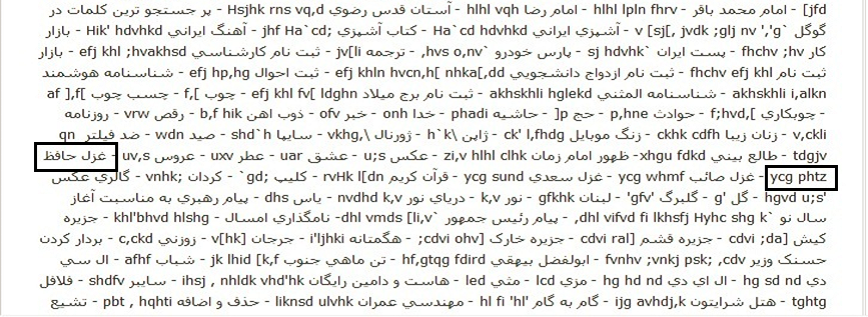
\includegraphics[scale=0.8]{Figures/persianwebdist.png}
\caption{\label{fig:plotdsc}
توزیع وب‌گاه‌های فارسی بر روی دامنه‌های مختلف در مجموعه داده‌ای \lr{PersianWebSpam-2013}
}
\end{figure}
\subsection{مجموعه ‌داده‌ای روش‌های مبتنی بر پیوند و روش ترکیبی}
به منظور ارزیابی روش‌های مبتنی بر پیوند و همچنین روش ترکیبی معرفی شده در این پژوهش، از دو مجموعه داده‌ای استاندارد \lr{WebSpamChallengeII-CorpusI} \cite{spam6} و \lr{WEBSPAM-UK2007} \cite{Yahooresearch} استفاده شده است. خصوصیات هر یک از این مجموعه‌های داده‌ای به شرح زیر می‌باشد:
\begin{itemize}
\item
مجموعه داده‌ای \lr{WebSpamChallengeII-CorpusI}: این مجموعه‌داده‌ای که مربوط به وب‌گاه‌های خزش شده در سال ۲۰۰۶ می‌باشد، در مسابقه‌ای به نام \lr{Web Spam Challenge II}‌\LTRfootnote{http://webspam.lip6.fr/wiki/pmwiki.php?n=Main.PhaseIITrainningCorpora/} در سال ۲۰۰۷ مورد استفاده قرار گرفته است. این مجموعه داده‌ای شامل ۹۰۷۲ وب‌گاه است که در این میان ۱۹۳۴ وب‌گاه (٪۲۱)، برچسب هرز و ۷۱۳۸ وب‌گاه (٪۷۹)، برچسب معتبر دارند. اطلاعاتی که از این مجموعه داده‌ای در اختیار شرکت‌کنندگان قرار گرفته است، گرافی شامل وب‌گاه‌های درون این مجموعه و پیوند بین آن‌ها، فایلی شامل اطلاعات مربوط به وزن \lr{TF-IDF} کلمات درون وب‌گاه‌ها و همچنین برچسب وب‌گاه‌ها می‌باشد. گراف مربوط به این وب‌گاه‌ها به صورت جهت‌دار و وزن‌دار می‌باشد که وزن هر یال، تعداد ارجاعات بین هر زوج صفحه متمایز از دو وب‌گاه را نشان می‌دهد. 
\item
مجموعه داده‌ای \lr{WEBSPAM-UK2007}: این مجموعه داده‌ای در می ۲۰۰۷ توسط گروهی در دانشگاه میلان \cite{Yahooresearch} جمع‌آوری شده است. این مجموعه داده‌ای شامل ۱۱۴۵۲۹ وب‌گاه از دامنه \lr{.uk} است که در مجموع دارای ۱۰۵۸۹۶۵۵۵ صفحه می‌باشند. از میان ۱۱۴۵۲۹ وب‌گاه موجود در این مجموعه داده‌‌ای، ۶۴۷۹ وب‌گاه برچسب‌گذاری شده‌اند که از میان آن‌ها 5709 وب‌گاه معتبر و 344 وب‌گاه هرز می‌باشد. 426 وب‌گاه باقی‌مانده نیز برچسب \mls{خط مرزی} خورده‌اند که نشان‌گر صفحاتی است که نمی‌توان در مورد هرز بودن یا نبودن آن‌ها قضاوت کرد. آن چه که از این مجموعه داده‌ای در اختیار پژوهشگران قرار گرفته است، مجموعه‌ای از ویژگی‌های محتوایی و پیوندی و همچنین گراف بین وب‌گاه‌های این مجموعه داده‌ای می‌باشد. مجموعه ویژگی‌‌های محتوایی این مجموعه داده‌ای، شامل ۹۶ ویژگی می‌باشد که برای تعداد زیادی از وب‌گاه‌ها از قبل محاسبه شده‌اند. در میان این ویژگی‌های محتوایی تنها تعداد محدودی از ویژگی‌‌‌ها جزء ویژگی‌هایی هستند که در این پژوهش مورد بررسی قرار گرفته‌اند. بنابراین به دلیل عدم امکان محاسبه سایر ویژگی‌های محتوایی، امکان استفاده از این مجموعه داده‌ای برای ارزیابی روش‌‌های محتوایی ارائه شده در این پژوهش وجود ندارد.
گراف این مجموعه داده‌ای نیز به صورت جهت‌دار و وزن‌دار بوده و وزن هر یال، تعداد ارجاعات صفحه یا صفحاتی از وب‌گاه مبدا به صفحه یا صفحاتی از وب‌گاه مقصد را مشخص می‌نماید. 
\end{itemize}

\section{معیار‌های ارزیابی}
\label{section:experiments-measures}
برای ارزیابی کیفیت روش‌های ارائه شده در این پژوهش، به ازای هر یک از روش‌های شناسایی هرز وب، از معیار‌های مشخصی استفاده شده‌ است که در ادامه به معرفی هر یک از آن‌ها می‌پردازیم.

\subsection{معیارهای ارزیابی وظیفه رده‌بندی هرز وب با استفاده از روش‌های مبتنی بر محتوا}
\label{subsection:experiments-measures-content}
به منظور ارزیابی روش‌هایی که برای رده‌بندی وب‌گاه‌های فارسی معرفی شده‌اند، از دو معیار دقت و فراخوانی برای هر دسته از صفحات هرز و معتبر استفاده شده است. برای محاسبه این دو معیار، ابتدا باید چهار پارامتر \mls{مثبت-صحیح} (\lr{TP})، \mls{مثبت-کاذب} (\lr{FP})، \mls{منفی-صحیح} (\lr{TN}) و \mls{منفی-کاذب} (\lr{FN}) را محاسبه کنیم. با توجه به این‌که هدف اصلی در این پژوهش شناسایی وب‌گاه‌های هرز می‌باشد، رخداد مثبت، هرز بودن یک وب‌گاه در نظر گرفته شده است. با توجه به این تعریف، یک رخداد مثبت-صحیح به شرایطی گفته می‌شود که برچسب حقیقی یک وب‌گاه و برچسبی که رده‌بند به آن داده است هر دو هرز باشند. به عبارت دیگر، یک صفحه‌ هرز، توسط رده‌بند به درستی شناسایی شده باشد. همچنین رخداد مثبت-کاذب به شرایطی اطلاق می‌شود که یک وب‌گاه معتبر، به اشتباه توسط رده‌بند به عنوان یک وب‌گاه هرز برچسب‌گذاری شود. در صورتی که رده‌بند یک وب‌گاه معتبر را به درستی برچسب‌گذاری کند، حالت منفی-صحیح رخ داده است. حالت منفی-کاذب نیز به شرایطی گفته می‌شود که رده‌بند به اشتباه یک وب‌گاه هرز را معتبر تشخیص دهد. با توجه به این تعاریف، معیارهای دقت و فراخوانی برای وب‌گاه‌های هرز و معتبر به صورت زیر تعریف می‌شود:
  \begin{equation}
  	Spam\text{-}Precision = \frac{TP}{TP + FP}
    \label{eq:sPrecission}
  \end{equation} 
  \begin{equation}
  	Spam\text{-}Recall = \frac{TP}{TP + FN}
    \label{eq:sRecall}
  \end{equation}
  \begin{equation}
  	NonSpam\text{-}Precision = \frac{TN}{TN + FN}
    \label{eq:nsPrecission}
  \end{equation} 
  \begin{equation}
  	Nonspam\text{-}Recall = \frac{TN}{TN + FP}
    \label{eq:nsRecall}
  \end{equation}
 
لازم به ذکر است که، برخلاف بسیاری از روش‌‌های پیشین که این نکته را در نظر نگرفته‌اند، محاسبه این معیارها برای هر دو کلاس هرز و معتبر به صورت مجزا، امری ضروری می‌باشد. دلیل این امر، نامتوازن بودن تعداد وب‌گاه‌های هرز و معتبر است. به عبارت دیگر، نسبت تعداد وب‌گاه‌های معتبر به وب‌گاه‌های هرز در وب خیلی زیاد است. وجود این اختلاف باعث می‌شود که نتوانیم تحلیل درستی از میزان کارایی روش‌ها در رده‌بندی وب‌گاه‌ها به دو کلاس هرز و معتبر داشته باشیم. ضمن این‌که هدف اصلی ما شناسایی وب‌گاه‌های هرز می‌باشد که برای بررسی آن لازم است معیارهای دقت و فراخوانی برای این کلاس به طور مجزا محاسبه شود. همچنین، برای محاسبه تخمینی از کیفیت کلی رده‌بند، از معیار $F1$، که ترکیبی از دو معیار دقت و فراخوانی می‌باشد، استفاده شده است. مقدار این معیار، طبق رابطه \ref{eq:f1} محاسبه می‌شود.
\begin{equation}
  	F1\text{-}Score = \frac{2\;(Precision* Recall)}{(Precision+Recall)}
    \label{eq:f1}
  \end{equation}
  
\subsection{معیارهای ارزیابی شناسایی هرز وب با استفاده از روش‌های مبتنی بر پیوند و روش ترکیبی}
\label{subsection:experiments-measures-link}
الگوریتم‌هایی که در بخش‌های \ref{chapter:ٍlinkbased} و \ref{chapter:ٍcontentandlinkbased} ارائه شده‌اند، در نهایت به هر صفحه یک امتیاز ارزشمندی یا عدم ارزشمندی اختصاص می‌دهند. سپس، صفحات بر اساس امتیازی که می‌گیرند رتبه‌بندی می‌شوند. در این پژوهش، برای ارزیابی این روش‌ها از دو نوع معیار ضریب هرز و ضریب اعتماد استفاده شده است. معیار ضریب هرز، که در مقاله \cite{liu2013combating} معرفی شده است، برای ارزیابی روش‌های انتشار اعتماد استفاده می‌شود. در این الگوریتم‌ها، در صورتی که صفحات را به ترتیب امتیاز اعتمادی که بدست آورده‌اند به طور نزولی مرتب کنیم، هدف این است که صفحات معتبر در رتبه‌های بالاتر این فهرست قرار بگیرند. هر چقدر تعداد صفحات هرز در اوایل این فهرست کمتر باشد، میزان ضریب هرز نیز کمتر و توانایی الگوریتم در شناسایی هرز وب بیشتر است. با فرض این‌که صفحات به ترتیب $s_1$، $s_2$، $s_3$، ...، $s_n$ رتبه‌بندی شده‌اند، ضریب هرز به صورت زیر محاسبه می‌شود:

 \begin{equation}
  	SpamFactor = \frac{\sum\limits_{i=1}^n \omega(s_i)\times\frac{1}{i}}{\sum\limits_{i=1}^n\frac{1}{i}},
    \label{eq:spamfrac}
  \end{equation} 
به طوری‌که در صورتی که صفحه $s_i$ هرز باشد، مقدار $\omega(s_i)$ برابر با یک و در صورتی که معتبر باشد این مقدار برابر با صفر است. 

همچنین برای سنجش میزان توانایی روش‌های انتشار هرز، معیاری به نام ضریب اعتماد را معرفی می‌نماییم که مشخص می‌کند چه میزان از صفحات هرز با چه دقتی توسط این الگوریتم‌ها شناسایی می‌شوند. برای محاسبه این معیار نیز ابتدا صفحات بر حسب امتیاز هرز بودنشان به طور نزولی مرتب می‌شوند. با فرض این‌که ترتیب صفحات به صورت $p_1$، $p_2$، $p_3$، ...، $p_n$ باشد، ضریب اعتماد به صورت زیر محاسبه می‌شود:

 \begin{equation}
  	ConfidenceFactor = \frac{\sum\limits_{i=1}^n \omega(p_i)\times\frac{1}{i}}{\sum\limits_{i=1}^l\frac{1}{i}},
    \label{eq:conffrac}
  \end{equation} 
که در آن $l$ تعداد کل صفحات هرز می‌باشد. در این عبارت، مخرج کسر حالت بهینه رتبه‌بندی صفحات می‌باشد که در آن تمام صفحات هرز در بالاترین رتبه ممکن قرار می‌گیرند.

\section{نتایج آزمایش‌ها}
\label{section:experiments-results}
در این بخش، نتایج آزمایش‌های صورت گرفته بر روی روش‌های معرفی شده به منظور شناسایی هرز وب را ارائه داده و با استفاده از معیارهای ارزیابی که در بخش \ref{section:experiments-measures} توضیح داده شد، نتایج را بررسی، تحلیل و با یکدیگر مقایسه می‌نماییم.

\subsection{ارزیابی روش‌های مبتنی بر محتوا در شناسایی هرز وب فارسی}
\label{subsection:experiments-results-content}
با توجه به این‌که هدف از این بخش، تحلیل روش‌های مبتنی بر محتوا بر روی وب‌گاه‌های فارسی می‌باشد، از مجموعه داده‌ای \lr{PersianWebSpam-2013} که به منظور انجام این پژوهش ساخته شده، ‌استفاده شده است. صفحات موجود در این پیکره با استفاده از ابزار \lr{Lemur} \cite{lemur} نمایه‌سازی شده و تمام ویژگی‌های محتوایی بیان شده در بخش \ref{chapter:contentbased} از آن‌ها استخراج شده است. پس از آن، با استفاده از ویژگی‌های محتوایی استخراج شده و همچنین ابزار \lr{Weka} \cite{weka}، وب‌گاه‌های موجود در این مجموعه داده‌ای رده‌بندی شده‌اند. همچنین برای رده‌بندی وب‌گاه‌ها در \lr{PSD-SYS} از \lr{LIBSVM} \cite{libsvm}، که یک کتابخانه به زبان \lr{C++} است، استفاده کرده‌ایم. با توجه به این‌که روش کار ما در این بخش به صورت باسرپرست می‌باشد، برای افزایش دقت و اعتبار ارزیابی نتایج، از روش \mls{اعتبار سنجی متقاطع $k$-بخشی} استفاده شده است. بنابراین با در نظر گرفتن اندازه مجموعه داده‌ای، برای ارزیابی تمام روش‌های مبتنی بر محتوا از اعتبار سنجی ۵-بخشی استفاده کرده‌ایم. 

\subsubsection{ارزیابی مجموعه ویژگی‌های پایه}
به عنوان یک روش پایه، ابتدا ویژگی‌های معرفی شده در مقاله \cite{Ntoulas:2006} را که در بخش \ref{section:methodology-structuralcontentbased} به طور کامل توضیح دادیم استخراج کرده و با استفاده از انواع الگوریتم‌های یادگیری ماشین، وب‌گاه‌های فارسی موجود در پیکره را رده‌بندی کردیم. لازم به ذکر است که دو ویژگی مربوط به کلمات مشهور موجود در متن را، به ازای تعداد مختلف (۱۰۰، ۲۰۰، ۳۰۰، ۵۰۰ و ۱۰۰۰) کلمات مشهور محاسبه نمودیم. همچنین برای محاسبه مقدار دو ویژگی شباهت $n$-گرام‌ها، مقادیر مختلف ۱، ۲، ۳، ۴ و ۵ را برای احتمال مستقل و مقادیر ۲، ۳، ۴ و ۵ را برای احتمال وابسته در نظر گرفتیم.
نتایج رده‌بندهای مختلف با استفاده از مجموعه ویژگی‌های پایه در جدول \ref{table:fs1} ارائه شده است.
\begin{table}
\caption{\label{table:fs1}\small نتایج استفاده از الگوریتم‌های یادگیری ماشین برای رده‌بندی وب‌گاه‌های \lr{PersianWebSpam-2013} با استفاده از مجموعه ویژگی‌های پایه}
\begin{scriptsize}
\begin{center}
%\resizebox{\linewidth}{!}{
\begin{tabular}{|c||c|c|c||c|c|c|}
\hline
&\multicolumn{3}{c||}{\lr{\textbf{Spam}}}&\multicolumn{3}{c|}{\lr{\textbf{NonSpam}}}
\\
\cline{2-7}
\textbf{رده‌بند}&\lr{\textbf{Precision}}&\lr{\textbf{Recall}}&\lr{\textbf{F1}}
&\lr{\textbf{Precision}}&\lr{\textbf{Recall}}&\lr{\textbf{F1}}
\\
\hline\hline

\lr{\textbf{KNN}} & 43/33 & 40 & 41/45 & \textbf{83/2} & 84/86 & 84
\\
\hline
\lr{\textbf{Naive Bayes}} & 37/99 &  \textbf{40/33}  & 38/39 & 82/53 & 80/29 & 81/22
\\
\hline
\lr{\textbf{Logistic Regression}} &  61/37 & 26/33 &  35/77 &  81/87 & 94/76 & 87/8
\\
\hline
\lr{\textbf{C4.5}} &  52/1 & 34/33 &  40/65 &  82/81 & 90/29 & 86/33
\\
\hline
\lr{\textbf{SVM}} &  \textbf{70/25} & 9/67 &  16/31 &  79/28 & \textbf{98/67} & \textbf{87/91}
\\
\hline
\lr{\textbf{Random Forest}} &  52/36 & 34/67 &  \textbf{41/51} &  82/99 & 90/95 & 86/77
\\
\hline

\end{tabular}
\end{center}
\end{scriptsize}
\end{table}

با توجه به جدول \ref{table:fs1} مشاهده می‌نماییم که روش جنگل تصادفی بیشترین امتیاز $F1$ را برای کلاس هرز دارد. با توجه به اهمیت زیاد رده‌بندی وب‌گاه‌های هرز در این وظیفه، در ادامه برای رده‌بندی وب‌گاه‌ها از الگوریتم جنگل تصادفی استفاده می‌شود. جنگل تصادفی یک رده‌بند تجمیعی است که تعداد زیادی درخت تصمیم ایجاد کرده و برای برچسب‌گذاری یک نمونه‌ آزمون، از رای اکثریت استفاده می‌کند. با استفاده از این روش از فرابرازش داده‌ها جلوگیری شده و برچسب‌گذاری نمونه‌ها، تحت تاثیر داده‌های برون‌هشته قرار نمی‌گیرد. بنابراین استفاده از این روش برای رده‌بندی وب‌گاه‌های هرز که دارای مقادیر برون‌هشته زیادی برای ویژگی‌های مختلف هستند مناسب می‌باشد.

\subsubsection{ارزیابی مجموعه ویژگی‌های مکمل}
با توجه به این‌که صفحات وب از بخش‌های مختلفی تشکیل شده‌اند، هر کدام دارای خصوصیات زیادی هستند که می‌توان با استفاده از انواع ویژگی‌ها آن‌ها را شناسایی کرد. بنابراین در این بخش، ویژگی‌های مکملی که به مرور زمان در پژوهش‌های مختلف \cite{Fetterly:2004, Prieto:2013, Urvoy:2008tracking} معرفی شده است را از وب‌گاه‌های فارسی استخراج کرده و با استفاده از الگوریتم جنگل تصادفی وب‌گاه‌ها را رده‌بندی کردیم. نتایج این رده‌بندی در جدول \ref{table:fspairwise} ارائه شده است.

\begin{table}
\caption{\label{table:fspairwise}\small نتایج استفاده از مجموعه ویژگی‌های پایه، مکمل و جدید برای رده‌بندی وب‌گاه‌های موجود در مجموعه داده‌ای  \lr{PersianWebSpam-2013}}
\begin{scriptsize}
\begin{center}
\begin{tabular}{|c||c|c|c||c|c|c|}
\hline
&\multicolumn{3}{c||}{\lr{\textbf{Spam}}}&\multicolumn{3}{c|}{\lr{\textbf{NonSpam}}}
\\
\cline{2-7}
\textbf{ویژگی‌ها}&\lr{\textbf{Precision}}&\lr{\textbf{Recall}}&\lr{\textbf{F1}}
&\lr{\textbf{Precision}}&\lr{\textbf{Recall}}&\lr{\textbf{F1}}
\\
\hline\hline

\textbf{مجموعه ویژگی پایه} &  52/36 & 34/67 &  41/51 &  82/99 & 90/95 & 86/77
\\
\hline
\textbf{مجموعه ویژگی پایه و مکمل} & 68/99 &	48/67&	56/93&	86/51&	93/81&	90
\\
\hline
\textbf{مجموعه ویژگی پایه و جدید} &  66/56 	&49	&56/24	&86/43	&92/76&	89/47
\\
\hline
\textbf{مجموعه ویژگی پایه، مکمل و جدید} & \textbf{69/8}  &	\textbf{49}	 & \textbf{57/49}	&\textbf{86/55}	&\textbf{93/81}&	\textbf{90/03}
\\
\hline
\end{tabular}
\end{center}
\end{scriptsize}
\end{table}
با توجه به نتایج موجود در جدول \ref{table:fspairwise}، استفاده از ویژگی‌های مکمل، نتایج رده‌بندی محتوایی را از نظر معیار $F1$ برای کلاس هرز ٪۳۷/۱۵ و برای کلاس معتبر ٪۳/۷۲ بهبود داده است. 

\subsubsection{ارزیابی مجموعه ویژگی‌های جدید}
\label{subsubsection:experiments-results-content-fs3}
در این بخش، برای ارزیابی ویژگی‌های محتوایی جدیدی که در این پژوهش معرفی شده‌اند، آن‌ها را به مجموعه ویژگی‌های پایه اضافه کرده و نتایج رده‌بندی را بررسی می‌نماییم. نتایج این رده‌بندی در جدول \ref{table:fspairwise} ارائه شده است. با توجه به نتایج مشاهده می‌کنیم که با استفاده از این ویژگی‌های جدید محتوایی می‌توان نتایج رده‌بندی را به نسبت ویژگی‌های پایه ٪۳۵/۴۹ از نظر معیار $F1$ برای کلاس هرز و ٪۳/۱۱  برای کلاس معتبر بهبود داد. همان‌طور که واضح است این میزان بهبود بسیار نزدیک به میزان بهبودی است که با استفاده از ویژگی‌های مکمل در نتایج رده‌بندی ایجاد شده است. این امر نشان می‌دهد که میزان کارایی ویژگی‌های محتوایی جدیدی که در این پژوهش معرفی شده‌اند برابر با کارایی مجموعه ویژگی‌های مکملی است که تاکنون در پژوهش‌های مختلف ارائه شده است. این میزان بهبود در حالی است که تعداد ویژگی‌های محتوایی جدید تقریبا نصف تعداد ویژگی‌های مکمل است. همچنین هزینه محاسباتی این ویژگی‌های جدید نیز بسیار کمتر از هزینه محاسباتی بسیاری از ویژگی‌های پایه و مکمل می‌باشد.

پس از آن، ویژگی‌های محتوایی جدید را با دو مجموعه ویژگی پایه و مکمل ترکیب کرده و نتایج رده‌بندی را بررسی می‌نماییم. با توجه به جدول \ref{table:fspairwise} مشاهده می‌کنیم که ترکیب ویژگی‌های جدید با دو مجموعه ویژگی پایه و مکمل، نتایج رده‌بندی را از نظر معیار $Spam\text{-}F1$ حدود ٪۰/۹۸ بهبود داده است. همچنین این رده‌بند نهایی در مقایسه با رده‌بند پایه، ٪۳۸/۵ بهبود در معیار $Spam\text{-}F1$ و ٪۳/۷۶ بهبود در معیار $NonSpam\text{-}F1$ ایجاد کرده است.

اگرچه ترکیب ویژگی‌های جدید با دو مجموعه ویژگی پایه و مکمل، نتایج رده‌بندی وب‌گاه‌های فارسی را بهبود داده است اما استخراج تمام این ویژگی‌ها از مجموعه وب‌گاه‌ها، نیاز به صرف هزینه‌های محاسباتی و زمانی زیادی دارد. همچنین، ترکیب برخی از این ویژگی‌ها با یکدیگر باعث کاهش دقت رده‌بندی می‌شود. بنابراین برای رفع این مشکلات در ادامه از روش انتخاب ویژگی \lr{-test} $\chi^2$ استفاده شده است.

\subsubsection{نتایج روش انتخاب ویژگی و رده‌بندی نهایی}
\label{subsubsection:experiments-results-content-fsel}
در این مرحله، برای بهبود نتایج رده‌بندی و کاهش هزینه ابتدا، از روش \lr{-test} $\chi^2$ برای امتیازدهی به ویژگی‌ها استفاده شده است. پس از آن برای انتخاب زیرمجموعه‌ای از ویژگی‌های استخراج شده به عنوان ویژگی‌های بهینه، ابتدا تمام ویژگی‌ها را بر اساس امتیازی که از \lr{-test} $\chi^2$ بدست آورده‌اند، به صورت نزولی مرتب کرده و از روش حذف پس‌رو برای حذف ویژگی‌های غیربهینه استفاده کردیم. با استفاده از این روش، ابتدا رده‌بندی را با تمام ویژگی‌های استخراج شده از صفحات انجام داده و در هر مرحله به ترتیب، ویژگی با کمترین امتیاز \lr{-test} $\chi^2$ را از مجموعه ویژگی‌ها حذف کردیم. در صورتی که حذف ویژگی جدید باعث کاهش کیفیت نتایج رده‌بندی شده آن ویژگی را مجددا به مجموعه ویژگی‌های باقی‌مانده اضافه کردیم، در غیر این‌ صورت پس از حذف آن ویژگی، ویژگی بعدی را بررسی نمودیم. بدین ترتیب در نهایت تعدادی ویژگی به عنوان ویژگی‌های بهینه انتخاب شدند. این مجموعه ویژگی‌ها به همرا امتیاز \lr{-test} $\chi^2$ در جدول \ref{tab:fs} ارائه شده‌اند.
 
\begin{table}
\caption{\label{tab:fs}\small ویژگی‌های بهینه در شناسایی وب‌گاه‌های هرز فارسی}
\begin{scriptsize}
\begin{center}
\begin{tabular}{|c|c|c|}
\hline
\textbf{ویژگی}&\textbf{امتیاز $\chi^2$}&\textbf{رتبه}
\\
\hline
طول \lr{URL}	&194/884 &	1
\\
\hline
تعداد پیوندهای خروجی	&93/289	&2
\\
\hline
احتمال شباهت ۴-گرام‌های شرطی&81/623&3
\\
\hline
شباهت کسینوسی بین بدنه اصلی و متن پیوند با وزن‌دهی \lr{TF} &75/802&4
\\
\hline
احتمال شباهت 3-گرام‌های شرطی&61/497&5
\\
\hline
درصدی از صفحه که شامل ایست‌واژه‌ها است&59/187&6
\\
\hline
شباهت کسینوسی بین عنوان و متن پیوند با وزن‌دهی \lr{TF}&58/772&7
\\
\hline
درصد فشرده‌سازی&56/797&8
\\
\hline
شباهت کسینوسی بین متن پیوند و برچسب کلیدواژه‌ها و توضیحات با وزن‌دهی \lr{TF}&55/585&9
\\
\hline
تعداد \lr{i-frame}ها&54/39&10
\\
\hline
اندازه متن پیوند&52/467&11
\\
\hline
درصدی از صفحه که شامل ۱۰۰ کلمه مشهور پیکره است&39/729&12
\\
\hline
احتمال شباهت ۵-گرام‌های شرطی&39/408&13
\\
\hline
تعداد منابع چند‌رسانه‌ای&39/214&14
\\
\hline
تعداد عکس‌ها&39/209&15
\\
\hline
تعداد ابربرچسب‌های جاوا اسکریپت&37/842&16
\\
\hline
تعداد کلمات عنوان&34/436&17
\\
\hline
درصد متن پیوند درون صفحه&34/34&18
\\
\hline
تعداد کلمات درون ابربرچسب کلیدواژه‌ها و توضیحات&33/772&19
\\
\hline
شباهت کسینوسی بین بدنه اصلی و برچسب کلیدواژه‌ها و توضیحات با وزن‌دهی \lr{TF}&30/624&20
\\
\hline
متوسط طول کلمات&26/36&21
\\
\hline
تعداد کلمات بدنه اصلی&19/546&22
\\
\hline
تعداد کلمات صفحه&19/481&23
\\
\hline
احتمال شباهت ۵-گرام‌های مستقل&16/226&24
\\
\hline
\end{tabular}
\end{center}
\end{scriptsize}
\end{table}

همان‌طور که در جدول \ref{tab:fs} مشاهده می‌نماییم، از ۷ ویژگی معرفی شده در این پژوهش، ۵ ویژگی آن جزء مجموعه ویژگی‌های بهینه انتخاب شده است. 

در بین این ویژگی‌های بهینه، برای مشخص کردن تاثیر هر ویژگی در رده‌بندی، لازم است وزنی که رده‌بند به هریک از آن‌ها می‌دهد را محاسبه نماییم. همان‌طور که در جدول \ref{table:fs1} مشاهده کردیم، الگوریتم جنگل تصادفی بیشترین میزان $Spam\text{-}F1$ را در رده‌بندی وب‌گاه‌‌های فارسی با استفاده از ویژگی‌های معرفی شده دارد. همان‌طور که می‌دانیم در الگوریتم جنگل تصادفی تمام حالت‌های انتخاب ویژگی‌ها بر اساس اهمیتشان بررسی می‌شود و برچسب نمونه‌ها بر اساس رای اکثریت درخت‌ها مشخص می‌شود. در واقع این یکی از مزیت‌های الگوریتم جنگل تصادفی برای وظیفه شناسایی هرز وب می‌باشد، که تمام حالت‌های مختلف انتخاب زیر مجموعه‌ای از ویژگی‌ها و ترتیب استفاده از آن‌ها را در نظر می‌گیرد و به هر ویژگی به تنهایی یک وزن مشخصی نمی‌دهد. همان‌طور که \lr{Ntoulas} و همکاران نیز در مقاله \cite{Ntoulas:2006} بیان کرده‌اند، خصوصیات صفحات وب و ویژگی‌های محتوایی تعریف شده طوری می‌باشد که هر ویژگی به تنهایی تاثیر زیادی در شناسایی برچسب صفحات ندارد و برای محاسبه تاثیر آن‌ها لازم است تمام ویژگی‌ها در کنار هم در نظر گرفته شوند. با این حال اگر بخواهیم میزان تاثیر هر ویژگی را به طور مجزا در فرآیند رده‌بندی مشخص نماییم، می‌توان رده‌بندی را با استفاده از هر یک از ویژگی‌ها به طور مجزا انجام داده و با توجه به مقدار $Spam\text{-}F1$، میزان تاثیر هر ویژگی را در شناسایی وب‌گاه‌های هرز فارسی بررسی نماییم. با استفاده از این روش، ۱۵ ویژگی برتر به ترتیب بر اساس مقدار  $Spam\text{-}F1$ در جدول \ref{tab:feffect} ارائه شده‌اند.
\begin{table}
\caption{\label{tab:feffect}\small بررسی کارایی ویژگی‌های بهینه درشناسایی وب‌گاه‌های هرز}
\begin{scriptsize}
\begin{center}
\begin{tabular}{|c|c|c|}
\hline
\textbf{ویژگی}&\lr{\textbf{Spam-F1}}&\textbf{رتبه}
\\
\hline
طول \lr{URL}	&30/8 &	1
\\
\hline
احتمال شباهت 3-گرام‌های شرطی&29/1&2
\\
\hline
تعداد پیوندهای خروجی	&27/7	&3
\\
\hline
اندازه متن پیوند&26/9&4
\\
\hline
درصدی از صفحه که شامل ۱۰۰ کلمه مشهور پیکره است&26/9&5
\\
\hline
احتمال شباهت ۵-گرام‌های شرطی&26/5&6
\\
\hline
تعداد کلمات صفحه&26/2&7
\\
\hline
احتمال شباهت ۴-گرام‌های شرطی&25/9&8
\\
\hline
شباهت کسینوسی بین عنوان و متن پیوند با وزن‌دهی \lr{TF}&25/8&9
\\
\hline
شباهت کسینوسی بین بدنه اصلی و متن پیوند با وزن‌دهی \lr{TF} &25/8&10
\\
\hline
درصد فشرده‌سازی&25/7&11
\\
\hline
شباهت کسینوسی بین بدنه اصلی و برچسب کلیدواژه‌ها و توضیحات با وزن‌دهی \lr{TF}&24/7&12
\\
\hline
درصدی از صفحه که شامل ایست‌واژه‌ها است&24/6&13
\\
\hline
تعداد کلمات بدنه اصلی&24/3&14
\\
\hline
تعداد منابع چند‌رسانه‌ای&23/9&15
\\
\hline
\end{tabular}
\end{center}
\end{scriptsize}
\end{table}

با توجه به جدول \ref{tab:feffect}، موثرترین ویژگی محتوایی در رده‌بندی وب‌گاه‌های فارسی، طول \lr{URL} وب‌گاه‌ها می‌باشد. این امر بیان‌گر این نکته است که هرزنویسان برای ایجاد وب‌گاه‌های هرز فارسی از \lr{URL}هایی با تعداد زیادی کلیدواژه استفاده می‌کنند. دومین ویژگی موثر در شناسایی وب‌گاه‌های هرز، احتمال شرطی ۳-گرام‌ها می‌باشد. این ویژگی نشان می‌دهد که تعداد زیادی از وب‌گاه‌های هرز با استفاده از تکرار عبارت‌های ۳-گرامی تلاش می‌کنند رتبه‌شان را افزایش دهند. برای مثال عبارت «مدل لباس جدید»  در بسیاری از وب‌گاه‌های هرز به تعداد زیاد تکرار شده است. ویژگی سوم، تعداد پیوندهای خروجی می‌باشد. این امر نشان‌دهنده این مهم می‌باشد که وب‌گاه‌های هرز فارسی برای افزایش رتبه وب‌گاه‌های خود، تعداد زیادی از پیوندهای سایر وب‌گاه‌ها را درون صفحات خود قرار می‌دهند. ویژگی بعد، تعداد کلمات درون متن پیوند است که به طور متوسط در وب‌گاه‌های هرز بیشتر از وب‌گاه‌های معتبر می‌باشد. این وب‌گاه‌ها برای بالا بردن رتبه خود در میان نتایج پرس‌وجو‌ها، تعداد زیادی ارجاع به صفحات مختلف می‌دهند که هر کدام از آن‌ها شامل توضیحاتی پیرامون صفحه ارجاع داده شده و کلیدواژه‌های مربوط به آن‌ها می‌باشند. 

 پس از انتخاب مجموعه ویژگی‌های بهینه و حذف سایر ویژگی‌ها، نتایج رده‌بندی با استفاده از مجموعه ویژگی‌های بهینه بدست آمده‌ است. با توجه به جدول \ref{tab:fsresult} می‌توان مشاهده کرد که حذف ویژگی‌های غیربهینه از بردار ویژگی، نتایج رده‌بندی را به اندازه ٪۵/۹ از نظر معیار $Spam\text{-}F1$ و ۰/۷٪ از لحاظ معیار $NonSpam\text{-}F1$ بهبود داده است. علاوه بر این امر، در این روش با توجه به کاهش تعداد ویژگی‌ها، هزینه زمانی و محاسباتی کل فرآیند رده‌بندی نیز کاهش می‌یابد.
 \begin{table}
\caption{\label{tab:fsresult}\small نتایج استفاده از \lr{-test} $\chi^2$ در رده‌بندی وب‌گاه‌های \lr{PersianWebSpam-2013} }
\begin{scriptsize}
\begin{center}
\begin{tabular}{|c||c|c|c||c|c|c|}
\hline
&\multicolumn{3}{c||}{\lr{\textbf{Spam}}}&\multicolumn{3}{c|}{\lr{\textbf{NonSpam}}}
\\
\cline{2-7}
\textbf{ویژگی‌ها}&\lr{\textbf{Precision}}&\lr{\textbf{Recall}}&\lr{\textbf{F1}}
&\lr{\textbf{Precision}}&\lr{\textbf{Recall}}&\lr{\textbf{F1}}
\\
\hline\hline

\textbf{مجموعه ویژگی پایه، مکمل و جدید} &  69/8  	&49	&57/49&	86/552&	93/81&	90/029
\\
\hline
\textbf{مجموعه ویژگی‌های بهینه} & 72/48 	&52/67	&60/9	&87/45	&94/19	&90/69
\\
\hline
\end{tabular}
\end{center}
\end{scriptsize}
\end{table}


%نتایج مربوط به رده‌بندی وب‌گاه‌ها با استفاده از ویژگی‌های محتوایی پایه، مکمل و جدید، نشان می‌دهد که این ویژگی‌ها به تنهایی قادر به شناسایی تمام وب‌گاه‌های هرز فارسی نمی‌باشند. دلیل این امر، وجود انواع مختلفی از وب‌گاه‌های معتبر با خصوصیات متفاوت است که موجب می‌شود مرز خصوصیات ساختاری بین وب‌گاه‌های معتبر و هرز کم‌رنگ شود. از طرف دیگر به دلیل خصوصیات خاص وب‌گاه‌های فارسی است که نشان می‌دهد امروزه تعدادی از هرزنویسان برای مقابله با انواع روش‌های شناسایی هرز وب تلاش می‌کنند صفحات هرزی را ایجاد کنند که از لحاظ بسیاری از خصوصیات ساختاری مشابه وب‌گاه‌های معتبر باشند. آن‌ها با استفاده از این روش‌ سعی دارند روش‌های محتوایی شناسایی هرز وب را فریب دهند. از طرف دیگر، هرزنویسان برای بالا بردن رتبه وب‌گاه‌های خود، از تعداد زیادی کلیدواژه‌های رایج در پرس‌وجو‌ها استفاده می‌کنند. در این پژوهش، برای شناسایی این نوع از وب‌گاه‌ها سامانه‌ای به نام \lr{PSD-SYS} معرفی شده است.

\subsubsection{ارزیابی رده‌بندی وب‌گاه‌های فارسی با استفاده از \lr{PSD-SYS}}
\label{subsubsection:experiments-results-content-psdsys}
در این سامانه‌، پس از حذف ایست‌واژه‌ها و کلمات مربوط به ابربرچسب‌ها و نمایه‌سازی صفحات، کلمات رایج موجود در وب‌گاه‌های هرز مشخص شده و برای رده‌بندی وب‌گاه‌ها از مدل \lr{BOSW} استفاده شده است. تعداد ویژگی‌هایی که در این سامانه استخراج و استفاده می‌شود حدود ۳۵۰۰۰ ویژگی است که تعداد آن در مقایسه با تعداد وب‌گاه‌ها بسیار کمتر می‌باشد. در این بردار ویژگی، به ازای هر ویژگی مقدار صفر یا یک وجود دارد. همچنین پس از بررسی تعداد زیادی از الگوریتم‌های یادگیری ماشین، در نهایت برای رده‌بندی وب‌گاه‌ها از الگوریتم \lr{SVM} استفاده شده است. بدین منظور از ابزار \lr{LIBSVM} \cite{libsvm} با پارامترهای $c=10$ و $t=2$ استفاده شده است. جدول \ref{tab:bosw} نتایج رده‌بندی وب‌گاه‌های موجود در مجموعه ‌داده‌ای \lr{WebSpamPersian-2013} با استفاده از مدل \lr{BOSW} را با نتایج رده‌بندی آن‌ها با استفاده از مدل ساده کیف کلمات که در پژوهش‌های پیشین \cite{geng2013evaluating, Erdelyi:2011wsc, nikulin2010web} معرفی شده است، مقایسه می‌کند. 
\begin{table}
\caption{\label{tab:bosw}\small مقایسه رده‌بندی وب‌گاه‌های مجموعه داده‌ای \lr{WebSpamPersian-2013} با استفاده از مدل \lr{BOSW} و مدل کیف کلمات}
\begin{scriptsize}
\begin{center}
\begin{tabular}{|c||c|c|c||c|c|c|}
\hline
&\multicolumn{3}{c||}{\lr{\textbf{Spam}}}&\multicolumn{3}{c|}{\lr{\textbf{NonSpam}}}
\\
\cline{2-7}
\textbf{روش}&\lr{\textbf{Precision}}&\lr{\textbf{Recall}}&\lr{\textbf{F1}}
&\lr{\textbf{Precision}}&\lr{\textbf{Recall}}&\lr{\textbf{F1}}
\\
\hline\hline

\textbf{کیف کلمات} &  86/53 &	86/33&	86/35&	96/1&	96/09&	96/09
\\
\hline
\lr{\textbf{‌BOSW}} & 92/61&	86&	89/12&	96/08	&98&	97/03
\\
\hline
\end{tabular}
\end{center}
\end{scriptsize}
\end{table}

با توجه به جدول \ref{tab:bosw}، استفاده از روش \lr{BOSW} برای رده‌بندی وب‌گاه‌های فارسی نتایج رده‌بندی را به نسبت روش کیف کلمات ٪۳/۲۱ از نظر معیار $Spam\text{-}F1$ و ٪۰/۹۸ از نظر معیار $NonSpam\text{-}F1$ بهبود داده‌ است. با توجه به این نتایج مشاهده می‌کنیم که استفاده از روش \lr{BOSW} برای شناسایی وب‌گاه‌های فارسی بهتر از روش کیف کلمات می‌باشد. دلیل این امر این است که وب‌گاه‌های معتبر دارای موضوعات متنوعی هستند که در مجموع کلماتی که در این نوع از وب‌گاه‌ها هستند دارای پراکندگی زیاد و مربوط به موضوعات مختلف هستند. همان‌طور که توضیح داده شد، در روش کیف کلمات، تمام این مجموعه کلمات به همراه کلمات مربوط به وب‌گاه‌های هرز، به عنوان بردار ویژگی رده‌بندی انتخاب می‌شوند. انتخاب تمام این کلمات به عنوان ویژگی‌های رده‌بندی، علاوه بر افزایش هزینه رده‌بندی، باعث ایجاد خطاهایی در رده‌بندی می‌شود. از طرف دیگر، وب‌گاه‌های هرز معمولا دارای کلماتی پیرامون موضوعات محدود مانند کلمات تبلیغاتی مربوط به کالاهای تقلبی خاص یا کلمات مربوط به فروش محصولات و کلماتی از این قبیل می‌باشند که معمولا ترکیب خاصی از این کلمات در وب‌گاه‌های هرز مشاهده می‌شود. برای مثال در وب‌گاه‌های فارسی موجود در مجموعه داده‌ای \lr{WebSpamPersian-2013}، کلمات «خرید»، «محصول»، «اس‌ام‌اس»، «دانلود»، «تخفیف»، «ویژه»، «رایگان» و کلماتی از این قبیل بسیار رایج هستند. استفاده از این کلمات برای شناسایی وب‌گاه‌های هرز روش مناسبی می‌باشد. در صورتی که اگر کلمات وب‌گاه‌های معتبر نیز به این بردار ویژگی اضافه شوند، باعث می‌شود تعداد زیادی از وب‌گاه‌های معتبر به اشتباه به عنوان هرز شناسایی شوند. برای مثال در صورتی که یک وب‌گاه معتبر مورد سوء‌استفاده وب‌گاه‌های هرز قرار بگیرد و متن‌های این وب‌گاه، درون تعدادی از وب‌گاه‌های هرز رونوشت شود، الگوی مربوط به کلمات درون این وب‌گاه معتبر به عنوان مشخصه‌ای از وب‌گاه‌های هرز شناسایی شده و به آن صفحه به اشتباه برچسب هرز داده می‌شود.

همان‌طور که می‌دانیم برای رده‌بندی نمونه‌ها توسط الگوریتم \lr{SVM} از بردار ویژگی‌ استفاده می‌شود. در سامانه \lr{PSD-SYS}، این بردار شامل مجموعه‌ای از کلمات رایج در مجموعه صفحات هرز می‌باشد. این روش بر اساس این فرض ارائه شده است که صفحات هرز دارای مجموعه‌ای از کلمات هرز هستند که رخداد ترکیب خاصی از این کلمات در یک صفحه نشان‌گر هرز بودن آن صفحه است. احتمال وجود این ترکیب‌های خاص کلمات هرز، در صفحات معتبر بسیار کم می‌باشد. برای مثال کلمه‌ای مانند «کنکور» ممکن است هم در صفحات هرز هم معتبر وجود داشته‌باشد. وجود این کلمه در کنار کلماتی مانند «دست‌بند»، «خرید»، «لاغری»، «عکس»، «اس‌ام‌اس» و «گیاهی» که جزء کلمات هرز هستند، نشان‌گر یک صفحه هرز می‌باشد. در صورتی که اگر این کلمه به همراه کلماتی مانند «خواندن»، «برنامه‌ریزی»، «رشته»، «دانشگاه» و کلمات دیگری که جزء کلمات رایج هرز نمی‌باشند در صفحه ظاهر شود، این صفحه به عنوان یک صفحه معتبر شناسایی می‌شود. در رده‌بند \lr{SVM} که در این پژوهش از آن برای رده‌بندی وب‌گاه‌ها استفاده شده است، برخی از این ترکیب‌های خاص، همان \mls{بردارهای پشتیبان} هستند که برای جدا کردن فضای صفحات هرز و معتبر استفاده می‌شوند. در صورتی که با همان احتمال کم، تعدادی از صفحات معتبر دارای ترکیبی خاص از کلمات هرز باشند، به طوری‌که در رده‌بندی این صفحه با استفاده از بردار ویژگی مربوط به آن، رده‌بند نتواند فرقی بین این صفحه و صفحات هرز قائل شود، این صفحه به عنوان صفحه هرز برچسب گذاری می‌شود. برای مثال، ممکن است در بخش نظرات یک صفحه معتبر، هرزنویسان آدرس صفحات خود را به همراه توضیحاتی درباره صفحه خود که شامل کلمات تبلیغاتی زیادی است قرار داده باشند و تعداد این کلمات و ترکیب آن‌ها طوری باشد که احتمال هرز بودن آن صفحه بیشتر از اعتبار آن شود و در نتیجه صفحه به عنوان یک صفحه هرز شناسایی شود. اما همان‌طور که در نتایج جدول \ref{tab:bosw} مشاهده می‌نماییم، احتمال وجود چنین صفحاتی کم است. به عبارت دیگر $Spam\text{-}F1$ برای این روش برابر با 92/61 می‌باشد، بدین معنا که تنها حدود ۷/۵ درصد از صفحات معتبر با استفاده از این روش به اشتباه به عنوان هرز برچسب خورده‌اند. همان‌طور که در نتایج جدول \ref{tab:bosw} مشخص است، این مقدار خطا حدود نصف خطای موجود در روش کیف کلمات (با خطای 13/5 درصد) است.
%دلیل خطای زیاد در روش کیف کلمات نیز این است که زمانی که کلمات مربوط به وب‌گاه‌های معتبر نیز در بردار ویژگی در نظر گرفته می‌شود، تعدادی از صفحات معتبر که مورد تهاجم صفحات هرز قرار گرفته‌اند به اشتباه به عنوان هرز برچسب‌گذاری می‌شوند. برای مثال، در صورتی که تعدادی از وب‌گاه‌های هرز، متن‌های مربوط به یک سایت معتبر را درون صفحه خود رونوشت کنند، تعداد زیادی از این کلمات موجود در وب‌گاه معتبر به عنوان مشخصه‌ای از وب‌گاه‌های هرز شناخته شده و در نتیجه در فرآیند رده‌بندی وب‌گاه‌ها، در صورت وجود این کلمات در صفحه، آن صفحه به عنوان یک صفحه هرز معرفی می‌شود. 

در ادامه، در این سامانه برای کاهش تعداد ویژگی‌ها و کاهش هزینه‌های زمانی و محاسباتی از روش‌های مختلف انتخاب ویژگی استفاده شده است. نتایج اعمال روش‌های مختلف  انتخاب بردار ویژگی در جدول \ref{tab:boswfs} ارائه شده است. هر روش، به ازای مقادیر آستانه متفاوت آزمایش شده و نتیجه مربوط به مقدار بهینه آن در جدول گزارش شده است.

\begin{table}
\caption{\label{tab:boswfs}\small نتایج استفاده از روش‌های مختلف انتخاب ویژگی در \lr{PSD-SYS}}
\begin{scriptsize}
\begin{center}
\begin{tabular}{|c||c|c|c||c|c|c|}
\hline
&\multicolumn{3}{c||}{\lr{\textbf{Spam}}}&\multicolumn{3}{c|}{\lr{\textbf{NonSpam}}}
\\
\cline{2-7}
\textbf{روش}&\lr{\textbf{Precision}}&\lr{\textbf{Recall}}&\lr{\textbf{F1}}
&\lr{\textbf{Precision}}&\lr{\textbf{Recall}}&\lr{\textbf{F1}}
\\
\hline\hline

\textbf{انتخاب ۲-گرام‌ها بدون محدودیت} &  88/83&85/67&87/13&95/95&96/86&96/4
\\
\hline
\textbf{انتخاب ۲-گرام‌ها با تعداد تکرار ۵ و بیشتر} &  93/262&86/333&89/601&96/186&98/19&97/173
\\
\hline
\lr{\textbf{Mutual Information}} &  90/967&85/333&87/993&95/886&97/524&96/693
\\
\hline
\textbf{\lr{-test} $\chi^2$} & 91/519&87/667&89/467&96/526&97/619&97/063
\\
\hline
\textbf{انتخاب ۱-گرام‌ها با تعداد تکرار ۴ و بیشتر} &  93/454&88/333&90/767&96/722&98/19&97/446
\\
\hline
\textbf{انتخاب ۱-گرام‌ها بدون محدودیت} &  92/608&86&89/124&96/085&98&97/029
\\
\hline
\textbf{انتخاب ۱-گرام‌ها با \lr{TF-IDF} بزرگتر و یا مساوی ۲۰} & 92/675&86/667&89/52&96/262&98&97/119
\\
\hline
\end{tabular}
\end{center}
\end{scriptsize}
\end{table}

با توجه به این نتایج مشاهده می‌نماییم که استفاده از روش وزن‌دهی \lr{TF} و انتخاب ۱-گرام‌های رایج در وب‌گاه‌های هرز با تعداد تکرار بزرگتر و مساوی ۴ به عنوان بردار ویژگی، بهترین نتایج را از لحاظ معیار $F1$ برای هر دو کلاس هرز و معتبر دارد. با مقایسه نتایج این جدول با نتایج جدول \ref{tab:bosw} مشاهده می‌شود که روش انتخاب ویژگی و حذف ویژگی‌های غیربهینه، نتایج رده‌بندی را از لحاظ دو معیار $Spam\text{-}F1$ و $NonSpam\text{-}F1$  بهبود داده است. 

در نهایت، مقایسه نتایج حاصل از رده‌بندی وب‌گاه‌ها با استفاده از \lr{PSD-SYS} با نتایج جدول \ref{tab:fsresult}، نشان می‌دهد که استفاده از \lr{PSD-SYS} برای رده‌بندی وب‌گاه‌ها در مقایسه با روش محتوایی بخش \ref{section:methodology-structuralcontentbased}، نتایج رده‌بندی را ٪۴۶/۰۵ از لحاظ معیار $Spam\text{-}F1$ و ٪۷/۴۵ از لحاظ معیار $NonSpam\text{-}F1$ بهبود داده است. با توجه به این نتایج مشاهده می‌کنیم که استفاده از ویژگی‌های محتوایی مربوط به ساختار وب‌گاه‌ها در رده‌بندی آن‌ها کارایی بالایی ندارد. دلیل این امر، وجود انواع مختلفی از وب‌گاه‌های معتبر با خصوصیات متفاوت است که موجب می‌شود مرز خصوصیات ساختاری بین وب‌گاه‌های معتبر و هرز کم‌رنگ شود. همچنین امروزه بسیاری از هرزنویسان برای مقابله با انواع روش‌های شناسایی هرز وب تلاش می‌کنند صفحات هرزی را ایجاد کنند که از لحاظ بسیاری از خصوصیات ساختاری، مشابه وب‌گاه‌های معتبر هستند. آن‌ها با استفاده از این روش‌ سعی دارند روش‌های محتوایی شناسایی هرز وب را فریب دهند. از طرف دیگر، برای بالا بردن رتبه وب‌گاه‌های خود در میان نتایج پرس‌وجوها، از تعداد زیادی کلیدواژه‌های رایج در پرس‌وجو‌ها استفاده می‌کنند. همان‌طور که نتایج نشان می‌دهد، این نوع از وب‌گاه‌های هرز با استفاده از \lr{PSD-SYS} قابل شناسایی می‌باشند. 


\subsection{ارزیابی روش‌‌های مبتنی بر پیوند در شناسایی هرز وب}
\label{subsection:experiments-results-link}
در این بخش، نتایج مربوط به رتبه‌بندی وب‌گاه‌ها با استفاده از هر یک از الگوریتم‌های مبتنی بر پیوند \lr{WorthyRank} و \lr{JunkyRank} ارائه داده می‌شود. برای ارزیابی این روش‌ها، از دو مجموعه داده‌ای استاندارد \lr{WebSpamChallengeII-CorpusI} و \lr{WEBSPAM-UK2007} استفاده شده است. برای تحلیل میزان کارایی الگوریتم‌های معرفی شده، نتایج آن‌ها را با نتایج حاصل از تعدادی از روش‌های پیشین در این زمینه مقایسه می‌نماییم. بدین منظور، ابتدا به توضیح مختصر هر یک از روش‌های پایه پرداخته و سپس عملکرد آن‌ها را با عملکرد الگوریتم‌های معرفی شده در این پژوهش مقایسه می‌کنیم. 

\subsubsection{معرفی روش‌های پایه}
در این بخش، ابتدا تعدادی از روش‌های پیشین که به عنوان روش پایه این الگوریتم‌ها در نظر گرفته شده‌اند را به اختصار توضیح می‌دهیم.
\begin{itemize}
\item
الگوریتم \lr{TrustRank}: این الگوریتم که برای اولین بار توسط \lr{Gyongyi} و همکاران \cite{gyongyi2004combating} معرفی شده است، بر اساس این فرض است که صفحات معتبر در وب، با احتمال زیادی به صفحات معتبر ارجاع می‌دهند. بنابراین در این الگوریتم، امتیاز اعتماد صفحات از مجموعه‌ای از صفحات معتبر که به عنوان صفحات بذر انتخاب شده‌اند، در جهت یال‌های گراف به سایر صفحات گراف انتشار داده می‌شود. همچنین در هر تکرار الگوریتم، صفحات بذر علاوه بر امتیازی که از پیوندهای ورودی از صفحات همسایه کسب می‌کنند، وزن ثابتی از امتیاز اولیه‌شان را نیز دریافت می‌کنند. بدین ترتیب در نهایت برای هر گره در گراف، یک امتیاز اعتماد محاسبه می‌شود. رابطه \ref{eq:trust} نحوه انتشار و محاسبه این امتیاز را برای هر گره موجود در گراف وب نشان می‌دهد.
\begin{equation}
\vec{t} = \alpha * M^T*\vec{t} + (1-\alpha)*\vec{s}
	\label{eq:trust}
\end{equation}
در این رابطه، $\vec{t}$ بردار امتیاز اعتماد، $M$ ماتریس مجاورت به‌هنجار شده گراف وب، و $\alpha$ عامل میرایی می‌باشد. بردار $s$ نیر بردار به‌هنجار شده مقدار اولیه امتیاز اعتماد صفحات بذر است که در آن، در صورتی که $p$ عضوی از مجموعه صفحات بذر معتبر باشد $s(p)=\frac{1}{|S^\text{+}|}$، و در غیر این صورت برابر با صفر است.
\item
الگوریتم \lr{Anti-TrustRank}: فرض دیگری که بعدها برای رابطه بین صفحات وب در نظر گرفته شد، این است که صفحاتی که به یک صفحه هرز ارجاع داده‌اند با احتمال زیادی هرز هستند. با توجه به این قانون، الگوریتم \lr{Anti-TrustRank} \cite{krishnan2006web} مطرح شد که در آن، امتیاز هرز بودن مجموعه‌ای از صفحات بذر هرز، در خلاف جهت یال‌های گراف به سایر صفحات گراف انتشار داده می‌شود. در این الگوریتم نیز مانند الگوریتم \lr{TrustRank} به هر صفحه بذر، علاوه بر امتیازی که از سایر صفحات دریافت می‌کند، درصدی از امتیاز ثابت هرز بودن اختصاص داده می‌شود. نحوه انتشار امتیاز هرز در گراف وب با استفاده از این الگوریتم در رابطه \ref{eq:distrust} مشخص شده است.
\begin{equation}
\vec{d} = \alpha * M*\vec{d}+(1-\alpha)*\vec{s^\prime}
	\label{eq:distrust}
\end{equation}
در این رابطه، $\vec{d}$ بردار امتیاز هرز بودن، $M$ ماتریس مجاورت به‌هنجار شده گراف، و $\alpha$ عامل میرایی می‌باشد.  $\vec{s^\prime}$ نیز بردار به‌هنجار شده مقدار اولیه امتیاز هرز بودن صفحات بذر است که در آن، در صورتی که $p$ عضوی از مجموعه صفحات بذر هرز باشد $s^\prime(p)=\frac{1}{|S^\text{-}|}$، و در غیر این صورت برابر با صفر است.
\item
الگوریتم \lr{TDR}: این الگوریتم که در سال 2011 توسط \lr{Zhang} و همکاران \cite{zhang2011propagating} معرفی شده است، از انتشار هم‌زمان دو امتیاز اعتماد و عدم اعتماد در گراف وب استفاده می‌کند. فرض آن‌ها بر این است که هر صفحه می‌تواند هم‌زمان دارای دو امتیاز هرز و اعتبار به صورت مجزا از هم باشد. همچنین در این الگوریتم برای انتشار امتیاز از گره $i$ به گره $j$، احتمال اعتبار یا هرز بودن گره مقصد در نظر گرفته می‌شود. نویسندگان این مقاله عقیده دارند که میزان اعتبار (عدم اعتبار) یک صفحه، در مقدار وزن اعتباری (عدم اعتبار) که از سایر صفحات وب دریافت می‌کند تاثیر دارد. در این الگوریتم در هر بار تکرار، امتیاز اعتبار یا هرز بودن صفحات به ترتیب با استفاده از روابط \ref{eq:tr} و \ref{eq:dr} محاسبه می‌شود.
\begin{equation}
t(p) = \alpha * \frac{\beta t(p)}{\beta t(p)+(1-\beta)d(p)}* \sum_{q:q\to p}\frac{t(q)}{outDegree(q)} + (1-\alpha)s(p)
	\label{eq:tr}
\end{equation}
\begin{equation}
d(p) = \alpha ^\prime *\frac{(1-\beta) d(p)}{(1-\beta)d(p)+\beta t(p)}*\sum_{q:p\to q} \frac{d(q)}{inDegree(q)} + (1-\alpha ^\prime)s^\prime(p)
	\label{eq:dr}
\end{equation}
که دو پارامتر $\alpha$ و  $\alpha^\prime$ همان عامل میرایی با مقدار ۰/۸۵ می‌باشند. همچنین مقداری که در این پژوهش برای پارامتر $\beta$ در نظر گرفته شده است، مانند مقاله \cite{zhang2011propagating}، برابر با ۰/۵ می‌باشد. $s(p)$ و $s^\prime(p)$ نیز به ترتیب معادل دو پارامتر $s(p)$ و $s^\prime(p)$ در الگوریتم‌های \lr{TrustRank} و \lr{Anti-TrustRank}  هستند.
\item
الگوریتم \lr{GBR}: این الگوریتم مشابه الگوریتم \lr{TDR} است، با این تفاوت که در زمان انتشار امتیاز از گره $i$ به $j$، به جای در نظر گرفتن احتمال اعتبار (هرز بودن) گره مقصد، احتمال اعتبار (هرز بودن) گره مبدا در نظر گرفته می‌شود. \lr{Liu} و همکاران \cite{liu2013combating} عقیده دارند که وزن انتشار امتیاز اعتماد (عدم اعتماد) صفحات باید با توجه به میزان احتمال اعتماد (عدم اعتماد) صفحه مبدا کنترل شود. بدین معنا که صفحه‌ای که دارای اعتبار زیادی است می‌تواند بخش زیادی از این اعتبار را به صفحات همسایه انتقال دهد. همچنین یک صفحه هرز که امتیاز اعتبار زیادی ندارد، وزن کمی از آن را می‌تواند به صفحات همسایه دهد و در ازای آن، امتیاز هرز بودن این صفحه با وزن بیشتری به سمت صفحات همسایه انتشار داده می‌شود. روابط \ref{eq:gr} و \ref{eq:br} به ترتیب نحوه محاسبه هر یک از امتیازهای اعتبار و هرز بودن صفحات را نشان می‌دهند.
\begin{equation}
g(p) = \alpha \sum_{q:q\to p} \left( \frac{g(q)}{outDegree(q)}*\frac{g(q)}{g(q)+b(q)} \right) + (1-\alpha) s(p)
\label{eq:gr}
\end{equation}
\begin{equation}
b(p) = \alpha ^\prime \sum_{q:p \to q} \left( \frac{b(q)}{inDegree(q)}*\frac{b(q)}{g(q)+b(q)} \right) + (1-\alpha ^\prime) s^\prime (p)
\label{eq:br}
\end{equation}
مقادیر پارامترهای موجود در این دو رابطه نیز، معادل پارامترهای نظیر آن‌ها در روابط \ref{eq:tr} و \ref{eq:dr} می‌باشد.
\end{itemize}

همان‌طور که در بخش \ref{subsection:experiments-measures-link} توضیح داده شد، برای ارزیابی الگوریتم \lr{WorthyRank} از معیار ضریب هرز و برای ارزیابی الگوریتم \lr{JunkyRank} از ضریب اعتماد استفاده می‌نماییم. برای اجرای تمام الگوریتم‌ها از شرط همگرایی \ref{eq:convcond} با پارامتر $\epsilon = 0.1*10^{-9}$ و همچنین پارامتر $\alpha = 0.85$ به عنوان عامل میرایی استفاده شده است. 
%با در نظر گرفتن تعداد وب‌گاه‌های هر یک از دو مجموعه داده‌ای، تعداد وب‌گاه‌های بذر معتبر را برای مجموعه داده‌ای \lr{WEBSPAM-UK2007}، ۱۰۰۰ و برای مجموعه داده‌ای \lr{WebSpamChallengeII-CorpusI}، ۱۰۰ انتخاب کردیم. همچنین با توجه به این‌که درصد وب‌گاه‌های هرز کمتر از وب‌گاه‌های معتبر است، تعداد وب‌گاه‌های بذر هرز را برای این دو مجموعه داده‌ای، به ترتیب برابر با ۱۰۰ و ۱۰  در نظر گرفتیم.

\subsubsection{ارزیابی الگوریتم \lr{WorthyRank}}
برای ارزیابی الگوریتم \lr{WorthyRank}، آن را با سه روش پیشین \lr{TrustRank} در رابطه \ref{eq:trust}، \lr{TRank} در رابطه \ref{eq:tr}، و \lr{GRank} در رابطه \ref{eq:gr} مقایسه می‌نماییم. نتایج هر یک از این روش‌ها در جدول \ref{tab:worthy} ارائه شده است.

\begin{table}
\caption{\label{tab:worthy}\small نتایج ارزیابی الگوریتم \lr{WorthyRank} در مقایسه با تعدادی از روش‌های پیشین مربوطه}
\begin{scriptsize}
\begin{center}
\begin{tabular}{c|c|c|c|c|}
 \cline{2-5}
 &  \multicolumn{4}{c|}{\textbf{ضریب هرز}} \\
\hline
\multicolumn{1}{|c|}{\textbf{مجموعه داده‌ای}}&\lr{\textbf{TrustRank}}& \lr{\textbf{TRank}} & \lr{\textbf{GRank}}&\lr{\textbf{WorthyRank}}
\\
\hline\hline
\multicolumn{1}{|c|}{\lr{\textbf{WEBSPAM-UK2007}}} &  0/0153 & 0/0149&0/0137&0/0086
\\
\hline
\multicolumn{1}{|c|}{\lr{\textbf{WebSpamChallengeII-CorpusI}}} &  0/0053 & 0/0056&0/0052&0/0043
\\
\hline
\end{tabular}
\end{center}
\end{scriptsize}
\end{table}

همان‌طور که مشاهده می‌نماییم، الگوریتم \lr{WorthyRank} در مقایسه با روش‌های پیشین، در شناسایی وب‌گاه‌های هرز عملکرد بهتری دارد. با استفاده از این روش، میزان خطا در رتبه‌بندی وب‌گاه‌‌های معتبر به مقدار قابل توجهی کاهش یافته است. در ادامه با توجه به نتایج جدول، دلایل ضعف و یا قوت هر یک از این روش‌ها را تحلیل می‌نماییم.

با توجه به جدول \ref{tab:worthy}، مقدار ضریب هرز در الگوریتم \lr{TrustRank} در اکثر موارد بیشتر از سایر الگوریتم‌ها می‌باشد. یکی از دلایل پایین بودن کیفیت رتبه‌بندی وب‌گاه‌ها در این الگوریتم، می‌تواند وجود یال‌های جعلی در گراف وب باشد که در این الگوریتم هیچ سیاستی برای مقابله با آن در نظر گرفته نشده است. در این الگوریتم، امتیاز اعتماد هر صفحه بدون توجه به میزان اعتبار پیوند بین دو صفحه، به طور مساوی بین صفحات همسایه خروجی تقسیم می‌شود. هرزنویسان با قرار دادن پیوند صفحات خود درون بخش‌هایی از صفحات معتبر (مانند بخش نظرات کاربران)، این الگوریتم را فریب داده و امتیاز اعتماد صفحات خود را افزایش می‌دهند. 

با توجه به نتایج جدول، الگوریتم \lr{TRank} توانسته است به نسبت الگوریتم \lr{TrustRank} ضریب هرز کمتری را بدست آورد. همان‌طور که توضیح داده شد، در این الگوریتم امتیاز اعتماد هر صفحه به نسبت احتمال اعتبار صفحه مقصد انتشار داده می‌شود. به عبارت دیگر، وزن یک یال در این الگوریتم، با استفاده از احتمال اعتبار صفحه مقصد مشخص می‌شود. مشکلی که در این روش وجود دارد این است که احتمال اعتباری که برای صفحات محاسبه می‌شود، همچنان با استفاده از ساختار گرافی وب می‌باشد. در این روش، با شروع از یک مجموعه بذر معتبر اولیه، انتشار امتیاز از این مجموعه صفحات به سایر صفحات، در حالی انجام می‌شود که امتیاز اعتماد اولیه صفحات مقصد مشخص نمی‌باشد. بنابراین، صفحات هرزی که پیوند صفحات خود را درون تعداد زیادی از صفحات معتبر قرار می‌دهند، با فریب این الگوریتم می‌توانند رتبه خوبی را در میان سایر صفحات بدست آورند. با مقایسه ضریب هرز این الگوریتم با ضریب هرز الگوریتم \lr{TrustRank} برای مجموعه داده‌ای \lr{WebSpamChallengeII-CorpusI}، مشاهده می‌شود که در مواردی که تعداد این نوع از صفحات هرز در گراف وب زیاد باشد، خطای این الگوریتم از الگوریتم \lr{TrustRank} نیز بیشتر می‌شود. بنابراین در الگوریتم \lr{TRank}، تاثیر منفی ناشی از وجود یال‌های جعلی در گراف وب، همچنان در انتشار امتیاز اعتماد از صفحه مبدا به صفحه مقصد وجود دارد.

برای حل این مشکل، الگوریتم \lr{GBR} معرفی شد که به جای استفاده از احتمال اعتبار صفحه مقصد، از احتمال اعتبار صفحه مبدا استفاده می‌کند. در این الگوریتم با شروع اجرای آن در تکرار اول، احتمال اعتبار مبدا همان امتیاز اعتماد صفحات بذر است که از قبل مشخص شده است. همچنین به این دلیل که این‌ صفحات به صورت دستی برچسب‌گذاری شده‌اند، احتمال اعتبار آن‌ها از دقت زیادی برخوردار است. با توجه به جدول \ref{tab:worthy} مشاهده می‌نماییم که ضریب هرز در این الگوریتم کمتر از دو روش \lr{TrustRank} و  \lr{TRank} می‌باشد. اما همچنان در این الگوریتم خطای ناشی از وجود یال‌‌های جعلی در گراف وب وجود دارد. 

در نهایت، با توجه به جدول \ref{tab:worthy}، مشاهده می‌نماییم که الگوریتم \lr{WorthyRank} که در این پژوهش معرفی شده است، نسبت به روش‌های پیشین کمترین ضریب هرز را بدست آورده است. دلیل این امر این است که در این الگوریتم، به جای انتشار امتیاز اعتماد با توجه به احتمال اعتبار صفحه مبدا یا مقصد، از احتمال اعتبار یال‌های گراف استفاده می‌شود. این اعتبار با توجه به سایر گره‌های همسایه و رابطه بین آن‌ها محاسبه می‌شود. در صورتی که در دو روش \lr{Trank} و \lr{Drank}، احتمال اعتبار تنها بر اساس یال‌های ورودی به یک صفحه محاسبه می‌شود و یک صفحه هرز می‌تواند به تنهایی با ایجاد یک ساختار پیوندی جعلی بین خود و سایر گره‌های گراف این دو الگوریتم را فریب دهد. در صورتی که در الگوریتم \lr{WorthyRank} با استفاده از اطلاعاتی که از گره‌های همسایه بدست می‌آید، احتمالی که برای اعتبار هر یال محاسبه می‌شود دقیق‌تر است.

\subsubsection{بررسی میزان کارایی بخش‌های مختلف الگوریتم \lr{WorthyRank}}
در الگوریتم \lr{WorthyRank} علاوه بر انتخاب بهینه بذر، از دو سیاست خاص، یکی برای وزن‌دهی به یال‌ها و دیگری برای بسط دوره‌ای بذر استفاده شده است. هر یک از این روش‌ها به تنهایی در بهبود الگوریتم‌های انتشار برچسب مانند \lr{TrustRank} تاثیرات مثبتی دارد که برای بررسی آن‌ها، هر یک را به طور مجزا در الگوریتم \lr{TrustRank} اعمال می‌نماییم. جدول \ref{tab:partsworthy} میزان تاثیر هر یک از بخش‌های اصلی الگوریتم \lr{WorthyRank} را در  ضریب هرز حاصل از رتبه‌بندی وب‌گاه‌های دو مجموعه داده‌ای \lr{WebSpamChallengeII-CorpusI} و \lr{WEBSPAM-UK2007} نشان می‌دهد. 
\begin{table}
\caption{\label{tab:partsworthy}\small تاثیر هر یک از بخش‌های الگوریتم \lr{WorthyRank} در کاهش ضریب هرز }
\begin{scriptsize}
\begin{center}
\begin{tabular}{c|c|c|c|c|}
 \cline{2-5}
 &  \multicolumn{4}{c|}{\textbf{ضریب هرز}} \\
\hline
\multicolumn{1}{|c|}{\textbf{مجموعه داده‌ای}}& \lr{\textbf{TrustRank}}&\textbf{وزن‌دهی به یال‌ها}&\textbf{بسط دوره‌ای بذر}&\textbf{وزن‌دهی به یال‌ها + بسط دوره‌ای بذر}
\\
\hline\hline
\multicolumn{1}{|c|}{\lr{\textbf{WEBSPAM-UK2007}}} &  0/0153 & 0/0091&0/0125&0/0086
\\
\hline
\multicolumn{1}{|c|}{\lr{\textbf{WebSpamChallengeII-CorpusI}}} &  0/0053 & 0/0043&0/0054&0/0043
\\
\hline
\end{tabular}
\end{center}
\end{scriptsize}
\end{table}

همان‌طور که در جدول \ref{tab:partsworthy} مشاهده می‌نماییم، تاثیر وزن‌دهی به یال‌های گراف، در بهبود نتایج رتبه‌بندی وب‌گاه‌ها، بیشتر از تاثیر بسط دوره‌ای بذر می‌باشد. همچنین در مورد مجموعه داده‌ای دوم نیز مشاهده می‌کنیم که اعمال بسط دوره‌ای بذر، بدون وزن‌دهی به یال‌ها، سبب افزایش اندک مقدار ضریب هرز شده است. دلیل افزایش خطا می‌تواند این امر باشد که با وجود یال‌های جعلی در گراف وب، تعدادی از وب‌گاه‌های هرز می‌توانند امتیاز اعتماد خود را افزایش داده و به عنوان بذر معتبر جدید به مجموعه وب‌گاه‌های بذر اولیه اضافه شوند. این دسته از وب‌گاه‌ها، وب‌گاه‌های هرزی هستند که پیوند صفحات خود را درون تعداد زیادی از صفحات معتبر قرار می‌دهند. هر اندازه صفحات هرز موجود در گراف، فاصله کمتری با صفحات بذر اولیه داشته باشند، مقدار این خطا بیشتر می‌شود. با توجه به این‌که در مجموعه داده‌ای دوم، متوسط فاصله گره‌ها از همدیگر کوتاه‌تر از متوسط فاصله گره‌ها در گراف مجموعه داده‌ای اول می‌باشد، احتمال ارتباط نزدیک‌تر صفحات هرز دارای یال‌های جعلی، با صفحات بذر معتبر بیشتر است. به همین دلیل، مقدار ضریب هرز برای این مجموعه داده‌ای، در روش بسط دوره‌ای بذر افزایش یافته است، که با توجه به نتایج جدول، این مشکل با وزن‌دهی به یال‌های گراف حل می‌شود.

\subsubsection{ارزیابی الگوریتم \lr{JunkyRank}}
در این بخش، برای ارزیابی الگوریتم \lr{JunkyRank} آن را با سه الگوریتم \lr{Anti-TrustRank}، \lr{DRank} و \lr{BRank} مقایسه می‌نماییم. جدول \ref{tab:junky} نتایج مربوط به اجرای این سه الگوریتم را بر روی دو مجموعه داده‌ای \lr{WebSpamChallengeII-CorpusI} و \lr{WEBSPAM-UK2007} نشان می‌دهد. 

\begin{table}
\caption{\label{tab:junky}\small نتایج ارزیابی الگوریتم \lr{JunkyRank} در مقایسه با تعدادی از روش‌های پیشین مربوطه}
\begin{scriptsize}
\begin{center}
\begin{tabular}{c|c|c|c|c|}
 \cline{2-5}
 &  \multicolumn{4}{c|}{\textbf{ضریب اعتماد}} \\
\hline
\multicolumn{1}{|c|}{\textbf{مجموعه داده‌ای}}&\lr{\textbf{Anti-TrustRank}}& \lr{\textbf{DRank}} & \lr{\textbf{BRank}}&\lr{\textbf{JunkyRank}}
\\
\hline\hline
\multicolumn{1}{|c|}{\lr{\textbf{WEBSPAM-UK2007}}} &  0/33 & 0/36&0/35&0/37
\\
\hline
\multicolumn{1}{|c|}{\lr{\textbf{WebSpamChallengeII-CorpusI}}} &  0/73 & 0/78&0/74&0/85
\\
\hline
\end{tabular}
\end{center}
\end{scriptsize}
\end{table}
با توجه به جدول \ref{tab:junky} مشاهده می‌کنیم که میزان ضریب اعتماد در رتبه‌بندی وب‌گاه‌ها با استفاده از الگوریتم \lr{JunkyRank} افزایش یافته است. همچنین با توجه به جدول، پس از این الگوریتم به ترتیب الگوریتم‌های \lr{DRank} و \lr{BRank} بهترین نتایج را داشته‌اند. دلیل ضعف الگوریتم \lr{Anti-TrustRank} به نسبت سایر روش‌ها، وجود صفحات هرزی است که پیوند صفحات خود را درون تعدادی از صفحات معتبر قرار می‌دهند. ایجاد چنین پیوندهایی باعث می‌شود که این صفحات، امتیاز هرز بودن خود را به صفحات معتبر انتقال داده و باعث افزایش رتبه هرز بودن صفحات معتبر و در نتیجه کاهش رتبه هرز بودن خود شوند. 

در الگوریتم \lr{DRank} در صورت وجود یال از گره $i$ به گره $j$، برای انتشار امتیاز از گره $j$ به گره $i$ احتمال هرز بودن گره $i$ در نظر گرفته می‌شود. با توجه به این احتمال، که در صورت معتبر بودن صفحه $i$ مقدار آن کم است، درصد کمی از امتیاز هرز بودن صفحه هرز $j$ به صفحه معتبر $i$ انتقال داده می‌شود. این مهم در حالی است که در الگوریتم \lr{BRank} به این دلیل که احتمال هرز بودن صفحه مبدا $(j)$ در نظر گرفته می‌شود، همچنان، وجود پیوندهای جعلی از صفحات معتبر به صفحات هرز در رتبه‌بندی وب‌گاه‌ها تاثیر منفی می‌گذارد. با این حال، این الگوریتم نسبت به روش \lr{Anti-TrustRank} بهتر عمل می‌کند. دلیل این امر، رفتار خاص وب‌گاه‌های هرز در گراف وب می‌باشد. همان‌طور که در بخش \ref{section:linkbased-twsp} نیز توضیح داده شد، در یک گراف وب صفحاتی که به یک صفحه هرز ارجاع می‌دهند، با احتمال زیادی خود نیز یک صفحه هرز می‌باشند. در الگوریتم \lr{BRank} نیز با در نظر گرفتن احتمال هرز بودن صفحه هرز $j$، امتیاز هرز بیشتری به صفحاتی که به این صفحه ارجاع داده‌اند و با احتمال زیادی هرز هستند، انتقال داده می‌شود.

مشکلی که در هر سه روش پیشین وجود دارد این است که هیچ یک از این الگوریتم‌ها احتمال هرز بودن صفحاتی که یک صفحه هرز به آن‌‌ها ارجاع داده است را در نظر نمی‌گیرند. در صورتی که در موارد زیادی، مانند صفحات درون دهکده‌های پیوندی، هر صفحه هرز دارای تعداد زیادی ارجاع به سایر صفحات هرز می‌باشد. با استفاده از این روش، هرزنویسان می‌توانند رتبه صفحات خود را افزایش دهند. 
در الگوریتم \lr{JunkyRank} برای مقابله با این نوع از صفحات هرز، امتیاز هرز بودن یک صفحه علاوه بر انتشار در خلاف جهت یال‌های گراف، به سمت صفحات همسایه خروجی نیز انتشار داده می‌شود. 
همان‌طور که نتایج جدول \ref{tab:junky} نیز نشان می‌دهد، با استفاده از این روش می‌توان کیفیت رتبه‌بندی وب‌گاه‌‌ها را بهبود داد. 

\subsection{ارزیابی روش ترکیبی محتوایی و پیوندی در شناسایی هرز وب}
\label{subsection:experiments-results-contentandlink}
در این بخش، نتایج مربوط به رتبه‌بندی وب‌گاه‌ها با استفاده از الگوریتم \lr{CLCRank} ارائه می‌شود. برای اجرای این الگوریتم که از ترکیب اطلاعات محتوایی و پیوندی استفاده می‌کند، از دو مجموعه داده‌ای استاندارد \lr{WebSpamChallengeII-CorpusI} و \lr{WEBSPAM-UK2007} استفاده شده است. همچنین، مقایسه نتایج بر اساس دو معیار ضریب هرز و ضریب اعتماد صورت می‌گیرد. برای ارزیابی الگوریتم \lr{CLCRank}، نتایج آن را با نتایج حاصل از بهترین روش ترکیبی معرفی شده در مقاله \cite{polar2012} مقایسه می‌نماییم. بدین منظور، ابتدا به توضیح مختصری پیرامون این روش ترکیبی به عنوان یک روش پایه می‌پردازیم. 
\subsubsection{معرفی روش پایه}
در این روش که در سال ۲۰۱۲ توسط \lr{Ortega} و همکاران \cite{polar2012} معرفی شده است، از سه روش برای ترکیب اطلاعات محتوایی با الگوریتم انتشار برچسب استفاده شده است که در این میان، روش \lr{CS-NS} بیشترین دقت را در رتبه‌بندی وب‌گاه‌های معتبر داشته است. در این روش، ابتدا برای هر صفحه مقدار برخی از ویژگی‌های محتوایی که با احتمال هرز بودن وب‌گاه‌ها رابطه مستقیم دارند، محاسبه شده و بردار $F_p$ برای هر صفحه $P$، با استفاده از مقادیر این ویژگی‌ها مقداردهی می‌شود. سپس امتیاز هرز بودن هر صفحه $P$ با استفاده از رابطه \ref{eq:spaminess} محاسبه می‌شود. 
\begin{equation}
\label{eq:spaminess}
spaminess(P) =  \sqrt {\sum_{h \in F_p} h^2}
\end{equation}

\lr{Ortega} و همکاران \cite{polar2012} با بررسی هزینه محاسباتی تعدادی از ویژگی‌های محتوایی، در نهایت دو ویژگی محتوایی «متوسط طول کلمات» و «درصد فشرده‌سازی صفحه» را به دلیل هزینه محاسباتی کم آن انتخاب نمودند. با داشتن احتمال هرز بودن صفحات، $N^-$ صفحه با بیشترین امتیاز هرز، به عنوان مجموعه صفحات بذر هرز ($S^-$) و $N^+$ صفحه با کمترین امتیاز هرز بودن، به عنوان مجموعه صفحات بذر معتبر ($S^+$) انتخاب می‌شوند. سپس وزن هر صفحه بذر معتبر و هرز $i$ به ترتیب با استفاده از روابط \ref{eq:clsg} و \ref{eq:clsb} محاسبه می‌شود:
%ویژگی‌های استخراج شده باید طوری باشند که مقدار آن‌‌ها، با میزان هرز بودن صفحات رابطه مستقیم داشته باشد. بنابراین در مقاله \cite{polar2012} از درصد فشرده‌سازی و متوسط طول کلمات موجود در صفحه استفاده شده است. دلیل انتخاب این دو ویژگی این است که این دو، به نسبت سایر ویژگی‌ها هزینه محاسباتی کمتری دارند. با فرض این‌که $M(p)$ بردار مربوط به مقادیر هر یک از این ویژگی‌های محتوایی برای صفحه $p$ باشد، امتیاز هرز بودن صفحه $p$ به صورت زیر محاسبه می‌شود:%
\begin{equation}
\label{eq:clsg}
  e_i^+=\begin{cases}
     \frac{spaminess(i)}{\sum_{j \in S^+} spaminess(j)},& \text{if} \; \;  i \in S^+\\
    0, & \text{otherwise}
  \end{cases}
\end{equation}

\begin{equation}
\label{eq:clsb}
  e_i^-=\begin{cases}
     \frac{spaminess(i)}{\sum_{j \in S^-} spaminess(j)},& \text{if} \; \;  i \in S^-\\
    0, & \text{otherwise}
  \end{cases}
\end{equation}

پس از آن، امتیازهای اعتبار و هرز محتوایی بدست آمده از روابط \ref{eq:clsg} و \ref{eq:clsb} به ترتیب با استفاده از روابط \ref{eq:pr+} و \ref{eq:pr-} در کل گراف انتشار می‌یابد.
\begin{equation}
\label{eq:pr+}
PR^+(p) = (1-\alpha) {e_i}^+ + \alpha \sum_{q: q\rightarrow p} \frac{PR^+(q)}{outDegree(q)}  
\end{equation}
\begin{equation}
\label{eq:pr-}
 PR^-(p) = (1-\alpha) {e_i}^- + \alpha \sum_{q: p\rightarrow q} \frac{PR^-(q)}{inDegree(q)}   
\end{equation}

در نهایت، امتیاز نهایی هر صفحه به صورت زیر محاسبه می‌شود:
\begin{equation}
\label{eq:pr+-}
 score(p) = PR^+(p) - PR^-(p)
\end{equation}


%برای اجرای الگوریتم ترکیبی \lr{CS-NS}، با توجه به محدودیتی که از اطلاعات مجموعه‌های داده‌ای در اختیار داریم، به جای استفاده از رابطه \ref{eq:spaminess} برای محاسبه امتیاز هرز بودن وب‌گاه‌ها، با استفاده از ویژگی‌های محتوایی که از هر مجموعه‌داده‌ای در اختیار داریم با استفاده از الگوریتم جنگل تصادفی آن‌ها را رده‌بندی کرده و احتمال هرز بودن هر کدام را بدست می‌آوریم. لازم به ذکر است که با توجه به این‌که تعداد ویژگی‌هایی که برای محاسبه احتمال هرز بودن وب‌گاه‌ها استفاده می‌کنیم را افزایش داده‌ایم، تغییری که در این مرحله در الگوریتم \lr{} ایجاد کرده‌ایم، باعث کاهش کارایی الگوریتم نمی‌شود. بنابراین با ایجاد این تغییر نیز همچنان این الگوریتم می‌تواند معیار خوبی برای ارزیابی الگوریتم ؟؟ باشد.
\subsubsection{ارزیابی روش \lr{CLCRank}}
برای اجرای الگوریتم‌‌های این بخش، از پارامتر $\alpha = 0/85$ به عنوان عامل میرایی و شرط همگرایی \ref{eq:convcond} با پارامتر  $\epsilon = 0.1*10^{-9}$ استفاده نمودیم. 
%همچنین، با توجه به تعداد وب‌گاه‌های درون هر یک از مجموعه‌های داده‌ای، برای مجموعه داده‌ای   \lr{WebSpamChallengeII-CorpusI}  تعداد ۱۰۰ وب‌گاه معتبر و ۱۰ وب‌گاه هرز، و برای مجموعه داده‌ای  \lr{WEBSPAM-UK2007}، ۱۰۰۰ وب‌گاه معتبر و ۱۰۰ وب‌گاه هرز را به عنوان مجموعه وب‌گاه‌های بذر در نظر گرفتیم.

نتایج مربوط به رتبه‌بندی وب‌گاه‌ها با استفاده از دو روش \lr{CLCRank} و \lr{CS-NS} در جدول \ref{tab:clc:w} ارائه شده است. این نتایج نشان می‌دهد که میزان خطا در رتبه‌بندی وب‌گاه‌های معتبر با استفاده از الگوریتم \lr{CLCRank} به میزان قابل توجهی کمتر از الگوریتم \lr{CS-NS} است. لازم به ذکر است که، همان‌طور که در بخش \ref{section:experiments-datasets} نیز توضیح داده شد، تنها اطلاعاتی که از  محتوای وب‌گاه‌های درون مجموعه داده‌ای \lr{WebSpamChallengeII-CorpusI} در اختیار داریم، وزن \lr{TF-IDF} کلمات درون هر وب‌گاه است. با استفاده از این وزن می‌توان درصد فشرده‌سازی هر وب‌گاه را محاسبه کرد. برای محاسبه این ویژگی، ابتدا مقدار \lr{TF} هر کلمه را حساب کرده، سپس مجموع \lr{TF} کلمات درون هر وب‌گاه را بر تعداد کلمات یکتای آن وب‌گاه تقسیم می‌نماییم.
همچنین، به دلیل محدودیت دسترسی به اطلاعات محتوایی، به جای استفاده از ویژگی «متوسط طول کلمات»، از ویژگی «تعداد کلمات درون وب‌گاه» استفاده کردیم. همان‌طور که در \cite{Ntoulas:2006} نیز نشان داده شده است، مقدار این ویژگی، مانند ویژگی «متوسط طول کلمات»، با احتمال هرز بودن وب‌گاه‌ها رابطه مستقیم دارد. همچنین هزینه محاسباتی این ویژگی نیز از ویژگی «متوسط طول کلمات» کمتر می‌باشد. بنابراین جایگزینی این ویژگی با ویژگی «متوسط طول کلمات»، در کارایی الگوریتم تاثیر منفی ندارد.
 
\begin{table}
\caption{\label{tab:clc:w}\small مقایسه ضریب هرز در روش  \lr{CLCRank} و روش پایه \lr{CS-NS}}
\begin{scriptsize}
\begin{center}
\begin{tabular}{c|c|c|}
 \cline{2-3}
 &  \multicolumn{2}{c|}{\textbf{ضریب هرز}} \\
\hline
\multicolumn{1}{|c|}{\textbf{مجموعه داده‌ای}}& \lr{CS-NS}&\lr{CLCRank}
\\
\hline\hline
\multicolumn{1}{|c|}{\lr{\textbf{WEBSPAM-UK2007}}} & 0/0338 & 0/0084
\\
\hline
\multicolumn{1}{|c|}{\lr{\textbf{WebSpamChallengeII-CorpusI}}} & 0/0067  &0/0042
\\
\hline
\end{tabular}
\end{center}
\end{scriptsize}
\end{table}
در ادامه، برای ارزیابی میزان کارایی الگوریتم \lr{CLCRank} در محاسبه امتیاز هرز بودن هر وب‌گاه، مقدار ضریب اعتماد این الگوریتم را با ضریب اعتماد بدست آمده از الگوریتم پایه \lr{CS-NS} مقایسه می‌نماییم. برای محاسبه ضریب اعتماد در الگوریتم \lr{CS-NS}، برای هر وب‌گاه امتیازی را در نظر می‌گیریم که با استفاده از رابطه \ref{eq:pr-+} بدست آمده است.
\begin{equation}
\label{eq:pr-+}
 score(p) = PR^-(p) - PR^+(p)
\end{equation}

جدول \ref{tab:clc:j} نتایج حاصل از رتبه‌بندی وب‌گاه‌ها با استفاده از دو الگوریتم \lr{CLCRank} و \lr{CS-NS} را نشان می‌دهد.
\begin{table}[h]
\caption{\label{tab:clc:j}\small مقایسه ضریب اعتماد در روش  \lr{CLCRank} و روش پایه \lr{CS-NS} }
\begin{scriptsize}
\begin{center}
\begin{tabular}{c|c|c|}
 \cline{2-3}
 &  \multicolumn{2}{c|}{\textbf{ضریب اعتماد}} \\
\hline
\multicolumn{1}{|c|}{\textbf{مجموعه داده‌ای}}& \lr{\textbf{CS-NS}}&\lr{\textbf{CLCRank}}
\\
\hline\hline
\multicolumn{1}{|c|}{\lr{\textbf{WEBSPAM-UK2007}}} & 0/33 & 0/40
\\
\hline
\multicolumn{1}{|c|}{\lr{\textbf{WebSpamChallengeII-CorpusI}}} &0/74   &0/89
\\
\hline
\end{tabular}
\end{center}
\end{scriptsize}
\end{table}

بررسی نتایج دو جدول \ref{tab:clc:w} و \ref{tab:clc:j} نشان می‌دهد که استفاده از روش ترکیبی \lr{CLCRank} کیفیت رتبه‌بندی وب‌گاه‌ها را به نسبت روش پایه \lr{CS-NS} به میزان قابل توجهی بهبود می‌دهد. 
همچنین مقایسه نتایج این بخش با نتایج بخش \ref{subsection:experiments-results-link}، نکاتی را پیرامون کارایی الگوریتم‌های ترکیبی نسبت به الگوریتم‌های پیوندی آشکار می‌سازد که در ادامه به شرح مهم‌ترین آن‌ها می‌پردازیم.

در مرحله اول، مقایسه نتایج مربوط به الگوریتم‌های \lr{WorthyRank} و \lr{JunkyRank} با نتایج حاصل از الگوریتم \lr{CLCRank} نشان می‌دهد که ترکیب اطلاعات محتوایی با روش‌های پیوندی، تاثیر قابل توجهی در بهبود کیفیت رتبه‌بندی وب‌گاه‌ها دارد. در الگوریتم   \lr{CLCRank} با استفاده از احتمال اعتبار (عدم اعتبار) محتوایی وب‌گاه‌ها، می‌توان میزان انتشار امتیاز اعتماد (عدم اعتماد) وب‌گاه‌ها را در طول هر مسیر کنترل کرد. با استفاده از این روش، از خطای ناشی از وجود یال‌های جعلی در گراف وب کاسته می‌شود.

از طرف دیگر، با مقایسه روش پایه ترکیبی \lr{CS-NS} با دو روش پایه مبتنی بر پیوند  \lr{TrustRank} و \lr{Anti-TrustRank}، مشاهده می‌نماییم که استفاده از روش ترکیبی \lr{CS-NS}، نه‌تنها تاثیر چندانی در بهبود معیار ضریب اعتماد ندارد، بلکه ضریب هرز را نیز که نشان‌گر میزان خطا در رتبه‌بندی وب‌گاه‌ها می‌باشد، افزایش داده است. یکی از دلایل مهم این امر، سیاست نامناسب انتخاب وب‌گاه‌های بذر در این الگوریتم می‌باشد. در این الگوریتم، انتخاب مجموعه وب‌گاه‌های بذر بر اساس ویژگی‌های محتوایی انجام می‌شود، در صورتی که کاربرد اصلی این وب‌گاه‌ها، در انتشار برچسب می‌باشد و بهتر است که بر اساس معیارهای مبتنی بر پیوند انتخاب شوند. بنابراین، اگرچه ممکن است یک وب‌گاه، با توجه به امتیاز محتوایی به عنوان یک وب‌گاه هرز شناسایی شود، اما این وب‌گاه لزوما یک بذر مناسب برای الگوریتم‌های انتشار برچسب نمی‌باشد. به عنوان مثال، این احتمال وجود دارد که این وب‌گاه مربوط به گره‌ای در گراف وب باشد که با سایر گره‌ها ارتباط زیادی ندارد. بدیهی است که چنین وب‌گاهی نمی‌تواند امتیاز خود را به طور بهینه در سراسر گراف وب انتشار دهد. به همین دلیل است که در الگوریتم \lr{CLCRank}، برای انتخاب بذر از روش‌های پیوندی مانند \lr{PageRank} استفاده می‌نماییم. 

مشکل دیگر این الگوریتم، نحوه ترکیب امتیاز محتوایی با روش پیوندی می‌باشد. در این الگوریتم، تنها از امتیاز محتوایی مربوط به وب‌گاه‌های بذر استفاده می‌شود و فقط این امتیازها در گراف انتشار داده می‌شوند. در صورتی که الگوریتم \lr{CLCRank}، از امتیاز محتوایی تمام وب‌گاه‌های درون گراف استفاده می‌کند. 

یکی از مشکلات اساسی‌ در الگوریتم \lr{CS-NS}، وزن‌دهی وب‌گاه‌های بذر معتبر بر اساس امتیاز هرز بودن آن‌ها است. با توجه به رابطه \ref{eq:clsg} مشاهده می‌نماییم که برای مقداردهی به وب‌گاه‌های بذر معتبر نیز مانند وب‌گاه‌های  هرز، از امتیاز هرز استفاده شده است؛ به عبارت دیگر، با توجه به این رابطه، هر میزان مقدار هرز بودن یک وب‌گاه معتبر بیشتر باشد، وزن اولیه آن وب‌گاه نیز بیشتر است. در صورتی که در مورد وب‌گاه‌های معتبر، عکس این امر صدق می‌کند. دلیل افزایش قابل توجه ضریب هرز در این الگوریتم نسبت به روش‌های قبلی نیز همین مساله می‌باشد.

\chapter{جمع‌بندی و نکته‌های پایانی}
\label{chapter:conclusion}
\thispagestyle{plain}
در این پژوهش، سعی کردیم تاثیر انواع ویژگی‌های محتوایی را در شناسایی وب‌گاه‌های هرز فارسی بررسی کرده و یک روش با کارایی بالا برای شناسایی این نوع از وب‌گاه‌ها ارائه دهیم. همچنین، با توجه به خصوصیات خاص وب‌گاه‌های هرز، دو روش مبتنی بر پیوند برای رتبه‌بندی وب‌گاه‌ها ارائه دادیم. در نهایت برای بهبود کیفیت رتبه‌بندی، روشی را معرفی کردیم که از ویژگی‌های محتوایی نیز در کنار ویژگی‌های پیوندی استفاده می‌کند. در این فصل، ابتدا مرور مختصری بر دستاوردهای این پژوهش داشته و در ادامه، به منظور بهبود و گسترش این پژوهش، پیشنهادهایی را برای کارهای آینده ارائه می‌دهیم. 

\section{دستاورد‌های پژوهش}
با توجه به نبود مطالعات گسترده در زمینه شناسایی و مقابله با وب‌گاه‌‌های هرز فارسی، در این پژوهش ابتدا به بررسی کارایی تعداد زیادی از ویژگی‌های محتوایی پیشین در شناسایی وب‌گاه‌های فارسی پرداختیم. بررسی این ویژگی‌‌ها بر روی وب‌گاه‌های فارسی نشان داده است که بسیاری از وب‌گاه‌های هرز فارسی دارای خصوصیاتی هستند که با استفاده از ویژگی‌های محتوایی مربوط به خصوصیات ساختاری وب‌گاه‌ها، قابل شناسایی نمی‌باشند. همچنین نشان دادیم که تعدادی از ویژگی‌های محتوایی در رده‌بندی وب‌گاه‌های فارسی تاثیر منفی داشته و باعث کاهش دقت رده‌بندی می‌شوند. برای بهبود کارایی رده‌بندی این نوع از وب‌گاه‌ها، تعدادی ویژگی محتوایی جدید معرفی کردیم. هر چند با استفاده از این ویژگی‌ها، کیفیت شناسایی وب‌گاه‌های هرز بهبود پیدا کرد، اما همچنان امکان شناسایی انواع خاصی از وب‌گاه‌های فارسی وجود نداشت. بنابراین، یک سامانه شناساگر هرز وب به نام \lr{PSD-SYS} را ارائه دادیم که از مدل جدیدی به نام \lr{BOSW} برای شناسایی وب‌گاه‌های هرز فارسی استفاده می‌کند. این سامانه، با استفاده از مدل \lr{BOSW}، که بر مبنای کلمات رایج در وب‌گاه‌های هرز است، توانسته است درصد زیادی از وب‌گاه‌‌های هرز فارسی را با دقت خوبی تشخیص دهد. از جمله مزایای این سامانه این است که علاوه بر عملکرد خوب در رده‌بندی وب‌گاه‌ها، به نسبت سایر روش‌های محتوایی هزینه زمانی و محاسباتی کمتری دارد. 

در ادامه، در این پژوهش به بررسی روش‌های مبتنی بر پیوند پرداخته و با یافتن نقاط ضعف الگوریتم‌هایی که تاکنون مطرح شده‌‌اند، دو روش مبتنی بر پیوند معرفی کردیم که مشکلات الگوریتم‌های پیشین را ندارند. 
در الگوریتم \lr{WorthyRank}، با استفاده از وزن‌دهی به یال‌های گراف و مشخص کردن میزان اعتبار آن‌ها، خطاهای ناشی از وجود پیوندهای جعلی را در گراف وب کاهش دادیم. مزیت دیگری که این روش نسبت به روش‌های پیشین دارد، نیمه‌سرپرست بودن این الگوریتم است که این امکان را می‌دهد که با داشتن تعداد محدودی از وب‌گاه‌های برچسب خورده، در هر تکرار الگوریتم به صورت خودکار تعدادی وب‌گاه جدید به مجموعه وب‌گاه‌های بذر اولیه اضافه شود. این روش برای وظیفه شناسایی هرز وب، که برچسب‌زنی وب‌گاه‌ها در آن کاری زمان‌بر و پرهزینه می‌باشد، بسیار مناسب است. 

در الگوریتم دیگری به نام \lr{JunkyRank}، نشان دادیم که امتیاز هرز بودن یک وب‌گاه، علاوه بر انتشار به صورت پس‌رو در گراف، باید به صورت پیش‌رو نیز انتشار داده شود. دلیل این امر، وجود صفحات هرزی است که بخشی از یک دهکده پیوندی می‌باشند. وجود دهکده پیوندی در میان وب‌گاه‌ها امری رایج است که توسط هرزنویسان و با هدف افزایش رتبه وب‌گاه‌های هرز ایجاد می‌شود. با استفاده از آزمایش‌هایی که بر روی این الگوریتم صورت گرفت، نشان دادیم که استفاده از این روش در مقایسه با روش‌هایی که امتیاز هرز را فقط به صورت پس‌رو در گراف وب انتشار می‌دهند، نتایج بهتری را در رده‌بندی وب‌گاه‌ها بدست می‌آورد.
% همچنین  می‌توان با استفاده از ترکیب خطی امتیاز هرز با امتیاز اعتباری که در الگوریتم \lr{WorthyRank} محاسبه می‌شود، برای بهبود کیفیت رتبه‌بندی وب‌گاه‌ها استفاده می‌کند.

در نهایت نیز یک الگوریتم به نام \lr{CLCRank} را پیشنهاد دادیم که در آن، علاوه بر استفاده از اطلاعات ساختاری گراف وب، از امتیازاتی که با استفاده از رده‌بند محتوایی برای وب‌گاه‌ها محاسبه شده است نیز استفاده می‌شود. با استفاده از این روش نشان دادیم که برای شناسایی بهتر وب‌گاه‌های هرز، به هر دو نوع اطلاعات محتوایی و پیوندی آن‌ها نیاز داریم. این امر به این دلیل است که هرزنویسان برای فریب موتورهای جست‌و‌جو، از روش‌های متفاوتی برای افزایش رتبه وب‌گاه‌های هرز استفاده می‌کنند. برای مثال، در حالی‌که در برخی از وب‌گاه‌های هرز، فقط از روش‌های محتوایی برای افزایش رتبه استفاده شده است؛ برخی دیگر، تنها از روش‌‌های پیوندی استفاده می‌کنند. بسیاری از وب‌گاه‌های هرز نیز از ترکیب روش‌های موجود، برای افزایش رتبه خود در میان نتایج موتورهای جست‌و‌جو استفاده می‌کنند.

یکی دیگر از دستاوردهای مهم این پژوهش، ساخت پیکره‌ای از وب‌گاه‌های فارسی برچسب‌خورده به نام \lr{PersianWebSpam-2013} می‌باشد. با توجه به نبود پژوهشی قابل توجه در زمینه شناسایی و مقابله با وب‌گاه‌های هرز فارسی، مجموعه داده‌ای مناسبی در این زمینه در دسترس نبود. بنابراین برای انجام این پژوهش، ابتدا به جمع‌آوری و ساخت یک مجموعه‌داده‌ای از وب‌گاه‌های فارسی، که شامل ۳۰۰ وب‌گاه‌ هرز و ۱۰۵۰ وب‌گاه معتبر می‌باشد، پرداخته شد. 

\section{کارهای آینده}
در این بخش، تعدادی از کارهای آتی که به منظور گسترش و بهبود هر یک از روش‌های معرفی شده در این پژوهش می‌توان انجام داد را معرفی می‌نماییم.

از جمله مهم‌ترین کارهایی که می‌توان در راستای بهبود کیفیت مطالعات انجام شده در زمینه شناسایی هرز وب فارسی انجام داد، گسترش مجموعه‌ داده‌ای \lr{PersianWebSpam-2013} و ایجاد یک مجموعه داده‌ای جامع‌تر، از وب‌گاه‌های هرز و معتبر فارسی می‌باشد. با توجه به این‌که با گذشت زمان انواع جدیدی از وب‌گاه‌های هرز ایجاد می‌شود، با استفاده از مجموعه‌های داده‌ای پیشین نمی‌توان ارزیابی درستی از روش‌های شناسایی هرز وب داشت. در مجموعه داده‌ای جدید، علاوه بر برچسب هرز و معتبر، می‌توان برچسب خط مرزی را نیز در نظر گرفت. این برچسب به صفحاتی داده می‌شود که نمی‌توان در مورد هرز بودن یا نبودن آن‌ها قضاوت کرد. با توجه به میزان قابل توجه این صفحات در وب، اضافه کردن برچسب مربوط به آن‌‌ها در رده‌بندی وب‌گاه‌ها، می‌تواند تاثیر قابل توجهی در بهبود کیفیت رده‌بندی وب‌گاه‌ها داشته باشد.

برای داشتن یک نمونه مناسب از گراف وب، امکان جدا کردن صفحات وب بر اساس زبان آن‌ها وجود ندارد و لازم است که در مرحله خزش، تمام صفحات و پیوندهای بین آن‌ها در نظر گرفته شود. سپس در مراحل بعد، می‌توان طی انجام فرآیند پیش‌پردازش داده‌ها، محدودیت‌‌هایی را با توجه به زبان صفحات اعمال کرد. همچنین در مرحله خزش نیز می‌توان با انتخاب صفحات بذر به زبان موردنظر، صفحات درون گراف را به سمت این نوع از صفحات متمایل کرد. با استفاده از این روش، می‌توان یک مجموعه‌داده‌ای مناسب شامل صفحات فارسی ایجاد کرد. با توجه به این‌که به دلیل محدودیت زمانی انجام این پژوهش و همچنین هزینه زمانی بالای برچسب‌گذاری صفحات، امکان ساخت و تکمیل  مجموعه داده‌ای با حجم زیاد وجود نداشت، امید است که بتوان برای پژوهش‌های بعدی یک مجموعه داده‌ای کامل شامل درصد زیادی از صفحات فارسی را تهیه کرده و در دسترس پژوهشگران قرار بدهیم.

یکی از مشکلاتی که در اکثر روش‌های محتوایی مطرح شده وجود دارد، ضرورت وجود مجموعه‌ای از صفحات برچسب‌خورده، به عنوان داده‌های آموزش می‌باشد. همان‌طور که می‌دانیم برچسب‌گذاری صفحات وب، کاری زما‌ن‌بر و پرهزینه می‌باشد. همچنین با توجه به سرعت زیاد تغییر محتوای صفحات، به‌روز رسانی داده‌های آموزش امری مهم می‌باشد. بنابراین با ارائه روش‌های بدون‌سرپرست، می‌توان هزینه ناشی از ساخت داده‌های آموزش را کاهش داد. علاوه بر این امر، با استفاده از روش‌های بدون‌سرپرست، خطای ناشی از سوگیری نتایج به سمت داده‌های آموزش حذف می‌شود.

همان‌طور که در بخش \ref{section:relatedwork-userfeedback} توضیح داده شد، یکی از روش‌های شناسایی هرز وب، استفاده از \mls{بازخورد}‌های کاربران و اطلاعات مربوط به تاریخچه رفتار آن‌ها نسبت به وب‌گاه‌‌های مختلف می‌باشد. برای مثال، با دانستن تعداد دفعاتی که کاربران بر روی پیوند یک وب‌گاه تلیک می‌کنند، و یا مدت زمانی که در آن وب‌گاه می‌مانند، می‌توان تخمینی از میزان مفید بودن محتوای آن وب‌گاه داشت. ترکیب این اطلاعات با روش‌هایی که در این پژوهش مورد بررسی قرار گرفته‌اند، می‌تواند در بهبود کارایی روش‌های شناسایی هرز وب تاثیر مثبت داشته باشد. همچنین، انواعی از صفحات هرز هستند که بخشی از محتوای آن‌ها، مانند عنوان صفحه و یا بخش ابربرچسب کلیدواژه‌ها و توضیحات، به صورت پویا ایجاد می‌شود. این صفحات، به صورت برخط و پویا، در زمان وارد کردن یک پرس‌وجو توسط کاربران، کلمات آن پرس‌وجو را درون صفحه خود تکرار می‌کنند. ارائه روش‌هایی برای شناسایی این نوع از صفحات هرز، از اهمیت ویژه‌ای برخوردار است.

یکی از سیاست‌‌هایی که در الگوریتم \lr{WorthyRank} برای بهبود کیفیت رتبه‌بندی وب‌گاه‌ها استفاده شد، محاسبه میزان اعتبار یال‌های درون گراف وب و وزن‌دهی آن‌ها بر اساس این میزان اعتبار می‌باشد. در این پژوهش برای وزن‌دهی به یال‌ها از ضریب جاکارد استفاده شده است. برای محاسبه این ضریب به ازای هر زوج گره، فقط همسایه‌های مستقیم دو گره و رابطه بین آن‌ها بررسی می‌شود. با توجه به گستردگی رابطه بین گره‌ها در گراف وب، استفاده از اطلاعات همسایه‌های سطح دو و بیشتر، می‌تواند باعث بهبود دقت وزن‌دهی یال‌های گراف شود.

%در روش ترکیبی \lr{CLCRank}، احتمال اعتبار محتوایی وب‌گاه‌ها، با استفاده از روش‌های محتوایی موجود محاسبه شده است. یکی از اقداماتی که می‌توان در راستای بهبود این روش انجام داد بررسی میزان تاثیر دقت محتوایی بر نتیجه نهایی رتبه‌بندی می‌باشد.یکی از مشکلاتی که هنگام \mls{نمونه‌برداری} از گراف وب ایجاد می‌شود، وجود وب‌گاه‌هایی است که به تازگی ایجاد شده و تعداد پیوندهای آن‌ها کم می‌باشد. این‌ نوع از وب‌گاه‌ها به دلیل داشتن ارتباط کم با سایر بخش‌های گراف وب، امکان













\newpage
\thispagestyle{empty}
\mbox{}

%  : \linespread{1.2}
\linespread{1}


\small{
\bibliographystyle{ieeetr-fa}
\renewcommand{\bibname}{مراجع}
\clearpage
\bibliography{ref}
\addcontentsline{toc}{chapter}{مراجع}
}

\newpage
\thispagestyle{empty}
\mbox{}
\begin{multicols}{2}
\begin{doublespace}

\glossarystyle{mylistLa}
\printglossary[type=latin]
\addcontentsline{toc}{chapter}{واژه‌نامه انگلیسی به فارسی}

\newpage
\thispagestyle{empty}
\mbox{}

\clearpage
\glossarystyle{mylistFa}
\printglossary[type=persian]
\addcontentsline{toc}{chapter}{واژه‌نامه فارسی به انگلیسی}
\end{doublespace}
\end{multicols}

\begin{latin}
\pagestyle{empty}


% LATIN ABSTRACT
\newpage
\thispagestyle{empty}
\mbox{}
\newpage
\vspace*{-2cm}
{\centering\small{\bf{Abstract}} \par \vskip .1cm}
\begin{doublespace} \normalsize

In recent years, due to the increasing amount of data available on the internet, the use of search engines to retrieve relevant information from the World Wide Web has become pervasive. Among the huge number of websites, the ones which succeed to appear more frequently and in higher ranks of search engine results would receive more visitors. So, spammers struggle to achieve a higher than deserved rank for their websites using some illegal techniques called web spamming. 
Although various methods have been used for combatting web spamming, we could basically categorize them into three groups: content-based methods, link-based methods, and the methods based on miscellaneous data. 
In this thesis, we focus on content-based and link-based methods, and also their combination.

Despite the existence of many spam detection methods, the search engines do not perform well in detecting Persian spam websites. Thus, in this thesis, after preparing a corpus of spam and non-spam Persian websites, we analyze the effectiveness of many previously proposed content-based features on detecting Persian spam websites. To improve the performance of classification, we present a number of new content-based features and examine a number of feature selection method. As another approach, we propose a new Persian spam detection system which uses an improved version of bag-of-words model and has better performance in detecting Persian web spam. Due to the prevalence of link-based spamming methods, we analyze some of these methods and propose two new algorithms which do not have the weaknesses of previous methods. In the first algorithm, to improve the process of label propagation, we use three mechanisms: optimized seed selection, edge weighting, and seed expansion. In the second algorithm, we improve the quality of websites ranking, using label propagation in both forward and backward directions. Finally, we propose a combined method, which uses the content-based probability of being spam (non-spam) to propagate the spam (non-spam) score of websites. Using this method, we increase the performance of ranking websites.
 
Finally, to evaluate the proposed methods and compare their performance with the existing methods for this task, we have conducted several experiments on different datasets. Experiment results indicate that the proposed methods have a good performance in detecting web spam.




\end{doublespace}
{\par\vspace{2mm}}
\noindent\textbf{Keywords: }\textit{Spamming, Web Spam, Spam Detection, Label Propagation, Content-Based Features}
% END OF LATIN ABSTRACT

\newpage
\mbox{}


%%%%%%%%%%%%%%%%%%%%%%%%%%%%%
% LATIN TITLE PAGE
%%%%%%%%%%%%%%%%%%%%%%%%%%%%%
\font\titlefont=cmssbx10 scaled 2074
\font\supervisorfont=cmbxti10
\newpage
\thispagestyle{empty}
\begin{center}
\begin{tabular}{lp{7cm}r}

\includegraphics[width=3.8cm]{Figures/eng.png} & & 
\includegraphics[width=2.8cm]{Figures/ut.png} \\
\end{tabular}

\vskip 1cm
\Large{\bfseries
University of Tehran \par
School of Electrical and Computer Engineering}
\large
\par
\vskip 1.5cm
\addtolength{\baselineskip}{5mm}
{\titlefont Detecting Persian Spam Web Pages} \par
\addtolength{\baselineskip}{-5mm}
\vskip 1cm
{\bfseries By}\par
{\Large\bfseries Elahe Rabbani}\par
\vskip 1cm
Supervisors: \\
{\supervisorfont\Large Dr. Azadeh Shakery} \\
%{\supervisorfont\Large Dr. Masoud Asadpour}%
\par
\vskip 2cm
{A thesis submitted to the Graduate Studies Office \\ in partial fulfillment of the requirements \\ for the degree of Master of Science \par
in
\par
\vskip .7cm
\large Computer Engineering}
\par
\vskip .04cm
{September 2014}
\par
\vfill
\end{center}
%%%%%%%%%%%%%%%%%%%%%%%%%%%%%
% END OF LATIN TITLE

\end{latin}
\end{document}‍
